\chapter{Examples of MSN Function Interpolation}
\label{chap:func_interp}

In this chapter we present results using the fast MSN algorithms.
We begin by interpolating smooth functions before
attempting to interpolate rough functions (discontinuous functions
or functions with infinite derivatives).
Unless otherwise stated, all computations will be performed
in double precision.
In 1D, we compare the results with Lagrange interpolation on
Chebyshev nodes.
In 2D, we will compare MSN with interpolation on a tensor grid of
Chebyshev nodes; this is computed using the 2D IDCT.
When comparing against rough functions, we use some standard
filters (discussed below).

\section{Functions for Smooth Interpolation}

The functions we will be approximating will be
%
\begin{align}
    f_{R}(x,y) &= \frac{1}{1+ R(x^2 + y - 0.3)^{2}}
       + \frac{1}{1+ R(x + y - 0.4)^{2}} \nonumber\\
       &\quad+ \frac{1}{1+ R(x + y^{2} - 0.5)^{2}}
       + \frac{1}{1+ R(x^{2} + y^{2} - 0.25)^{2}} \nonumber\\
    g_{R}(x) &= f_{R}(x,0.8).
\end{align}
%
$f_{R}$ is a complicated function: it has a Runge function
on one line, one circle, and two parabolas.
The function $g_{R}$ is a coordinate slice of $f_{R}$.

% Section: Results for Fast MSN Interpolation in 1D
% \ref{sec:vs_I_1d}
\section{Results for Fast MSN Interpolation in 1D for Smooth Functions}
\label{sec:vs_I_1d}

\subsection{Interpolation Comparison}

We begin by comparing results with MSN on Chebyshev nodes
with standard Chebyshev interpolation
in Fig.~\ref{fig:smooth_comparison_1d_runge};
this contains results for interpolation of $g_{25}$ and $g_{100}$.
The results for large $s$ values closely match the Chebyshev
interpolation; this makes sense because we are smoothly cutting off
the Chebyshev coefficients, and larger $s$ values lead to a sharper
cutoff.

% Print results for comparing MSN with 2D Runge function

\begin{figure}[p]
    \centering
    \begin{subfigure}{0.45\textwidth}
    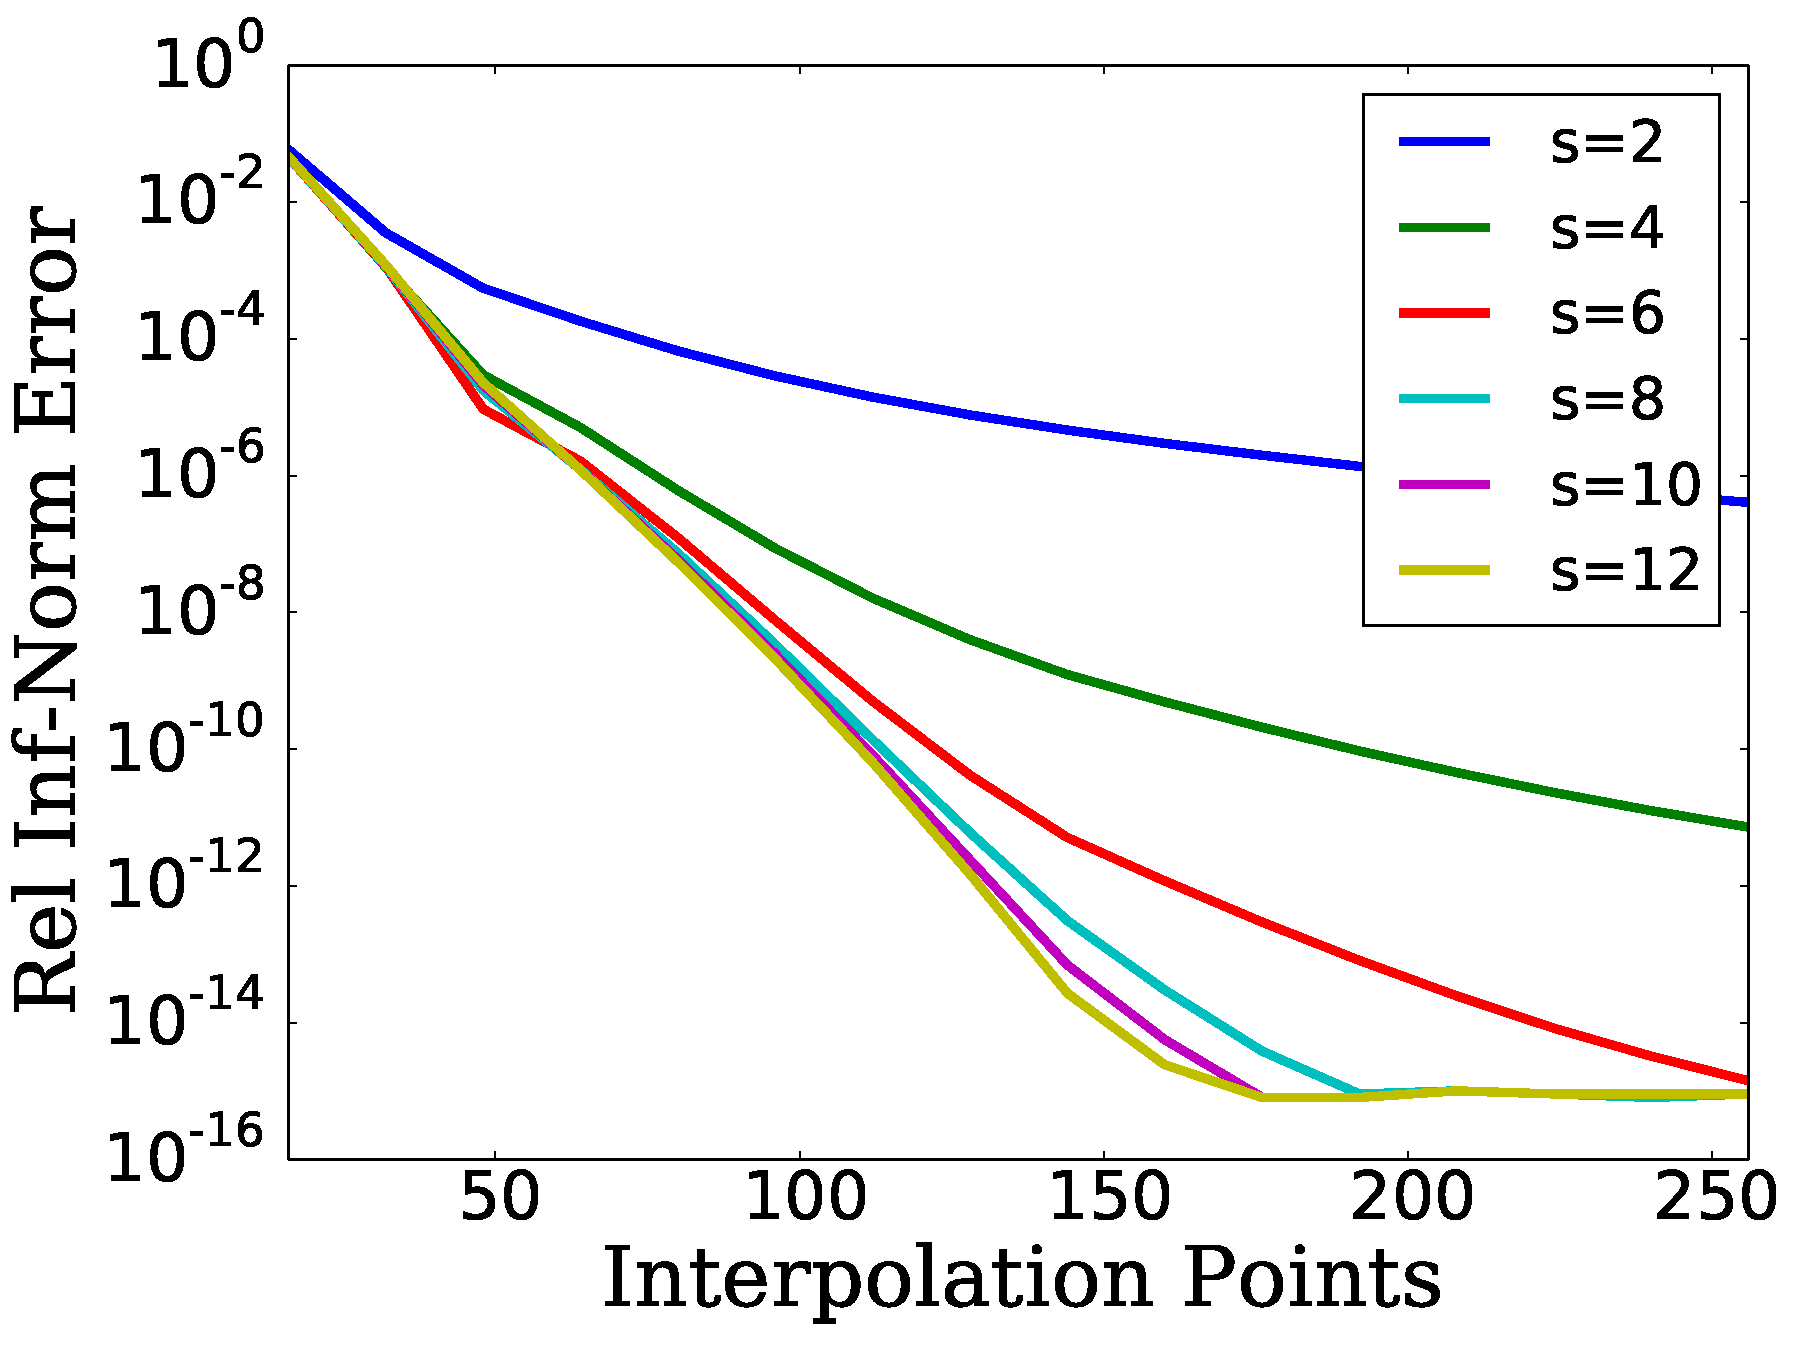
\includegraphics[width=\textwidth]{plots/msn_1d_smooth_R_25.pdf}
    \caption{$R=25$}
    \end{subfigure}
    \begin{subfigure}{0.45\textwidth}
    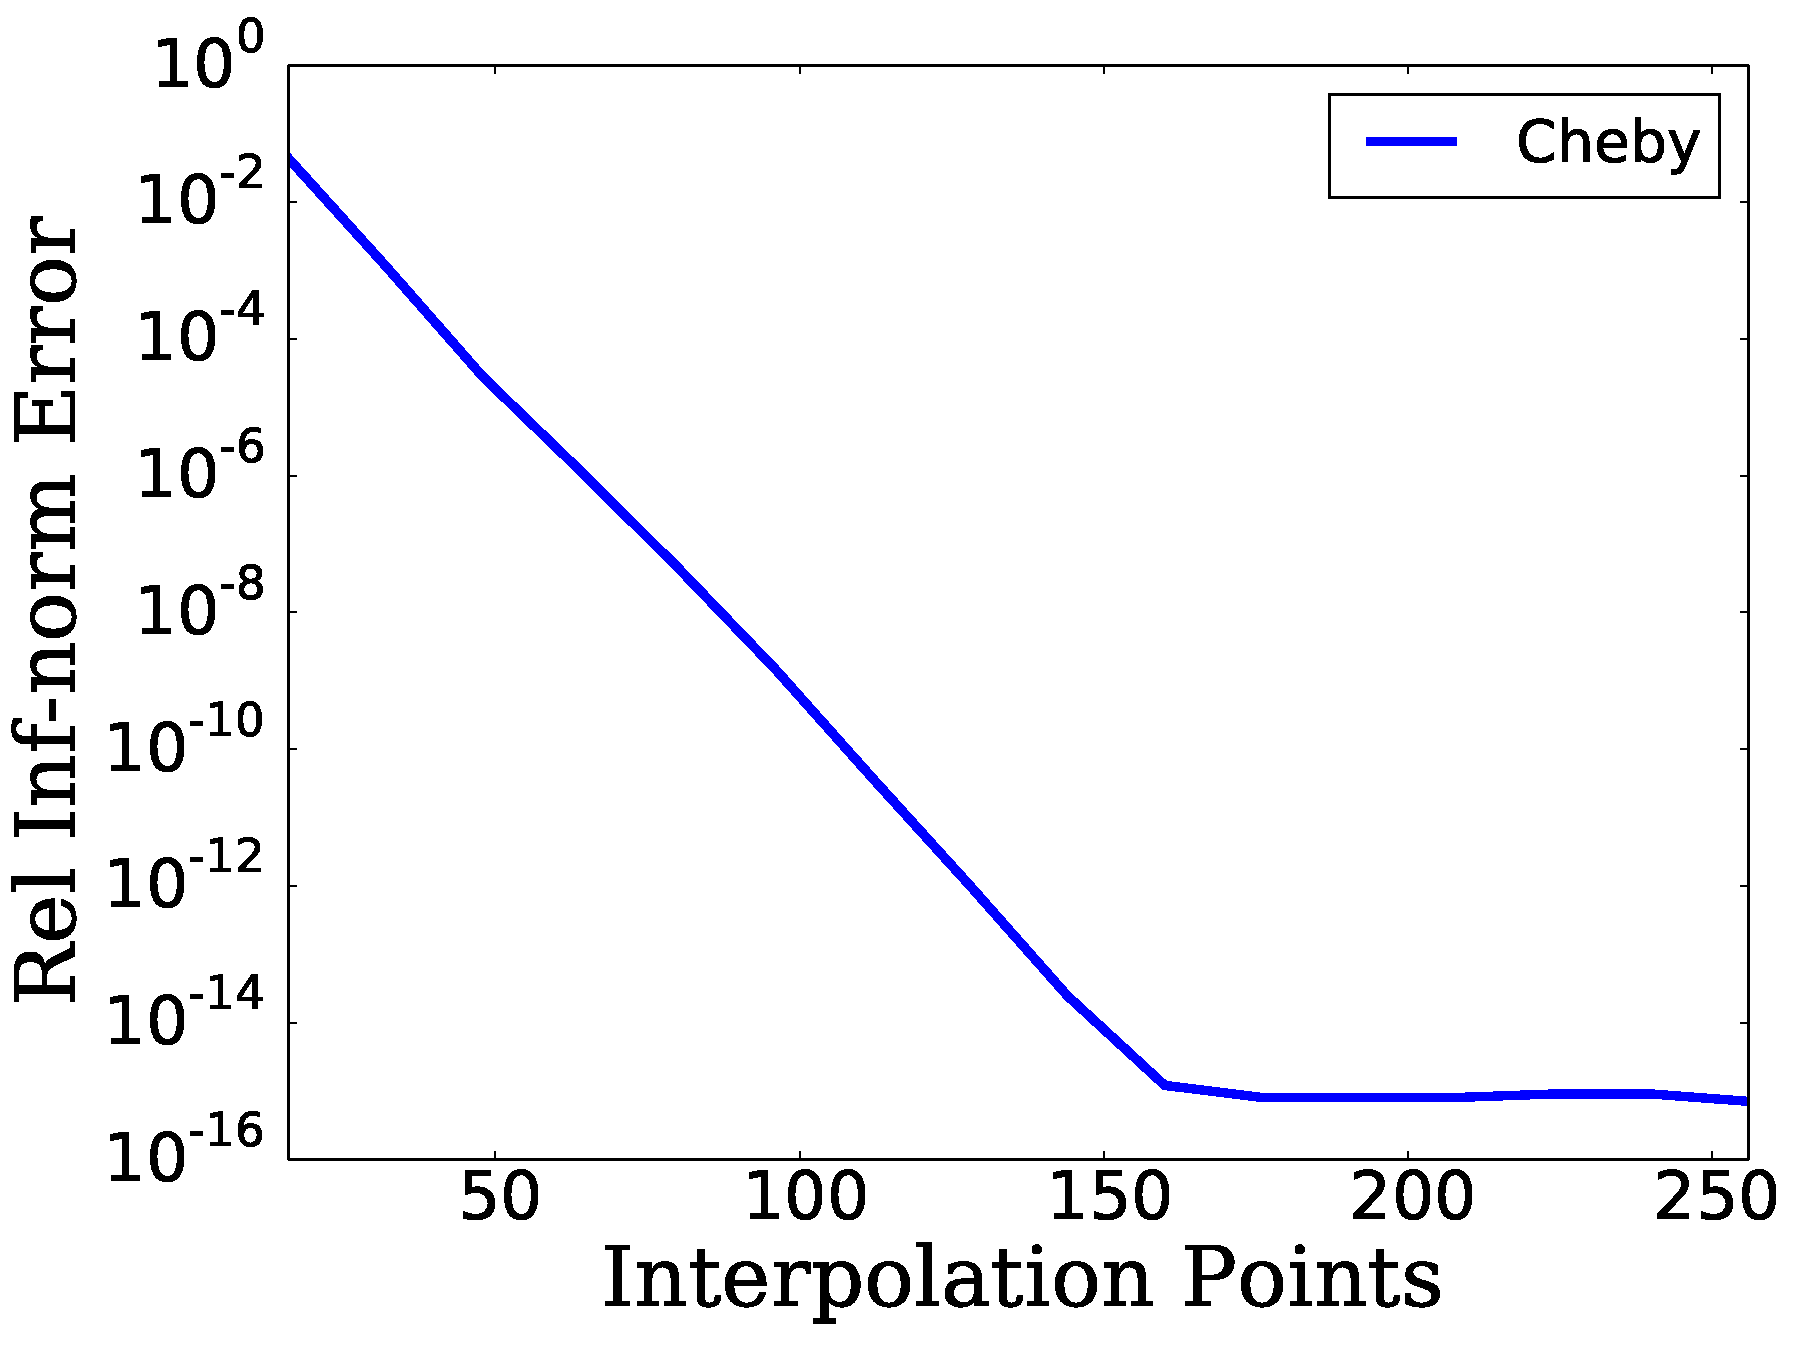
\includegraphics[width=\textwidth]{plots/cheby_1d_smooth_R_25.pdf}
    \caption{$R=25$}
    \end{subfigure}

    \begin{subfigure}{0.45\textwidth}
    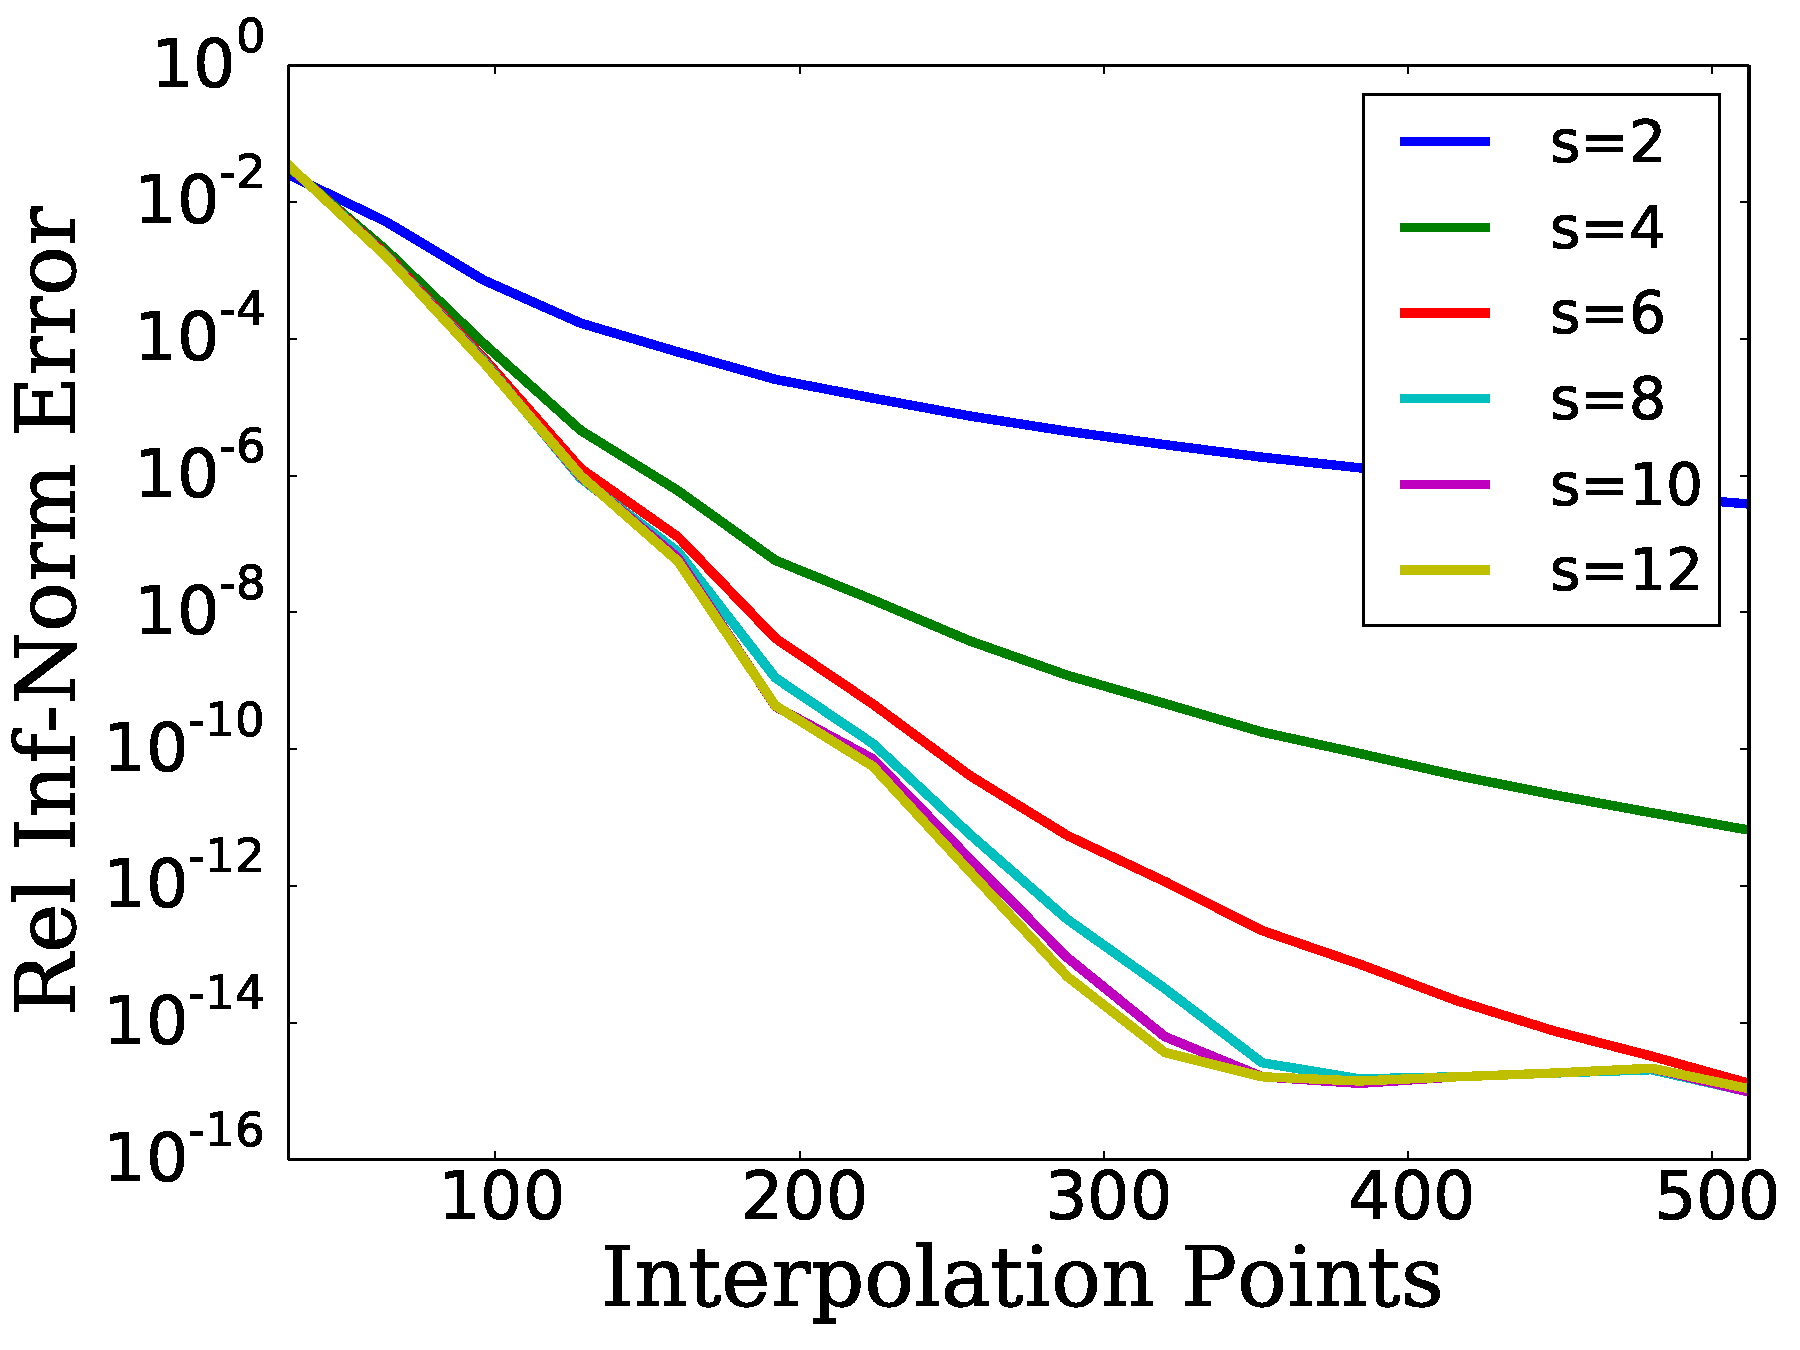
\includegraphics[width=\textwidth]{plots/msn_1d_smooth_R_100.pdf}
    \caption{$R=100$}
    \end{subfigure}
    \begin{subfigure}{0.45\textwidth}
    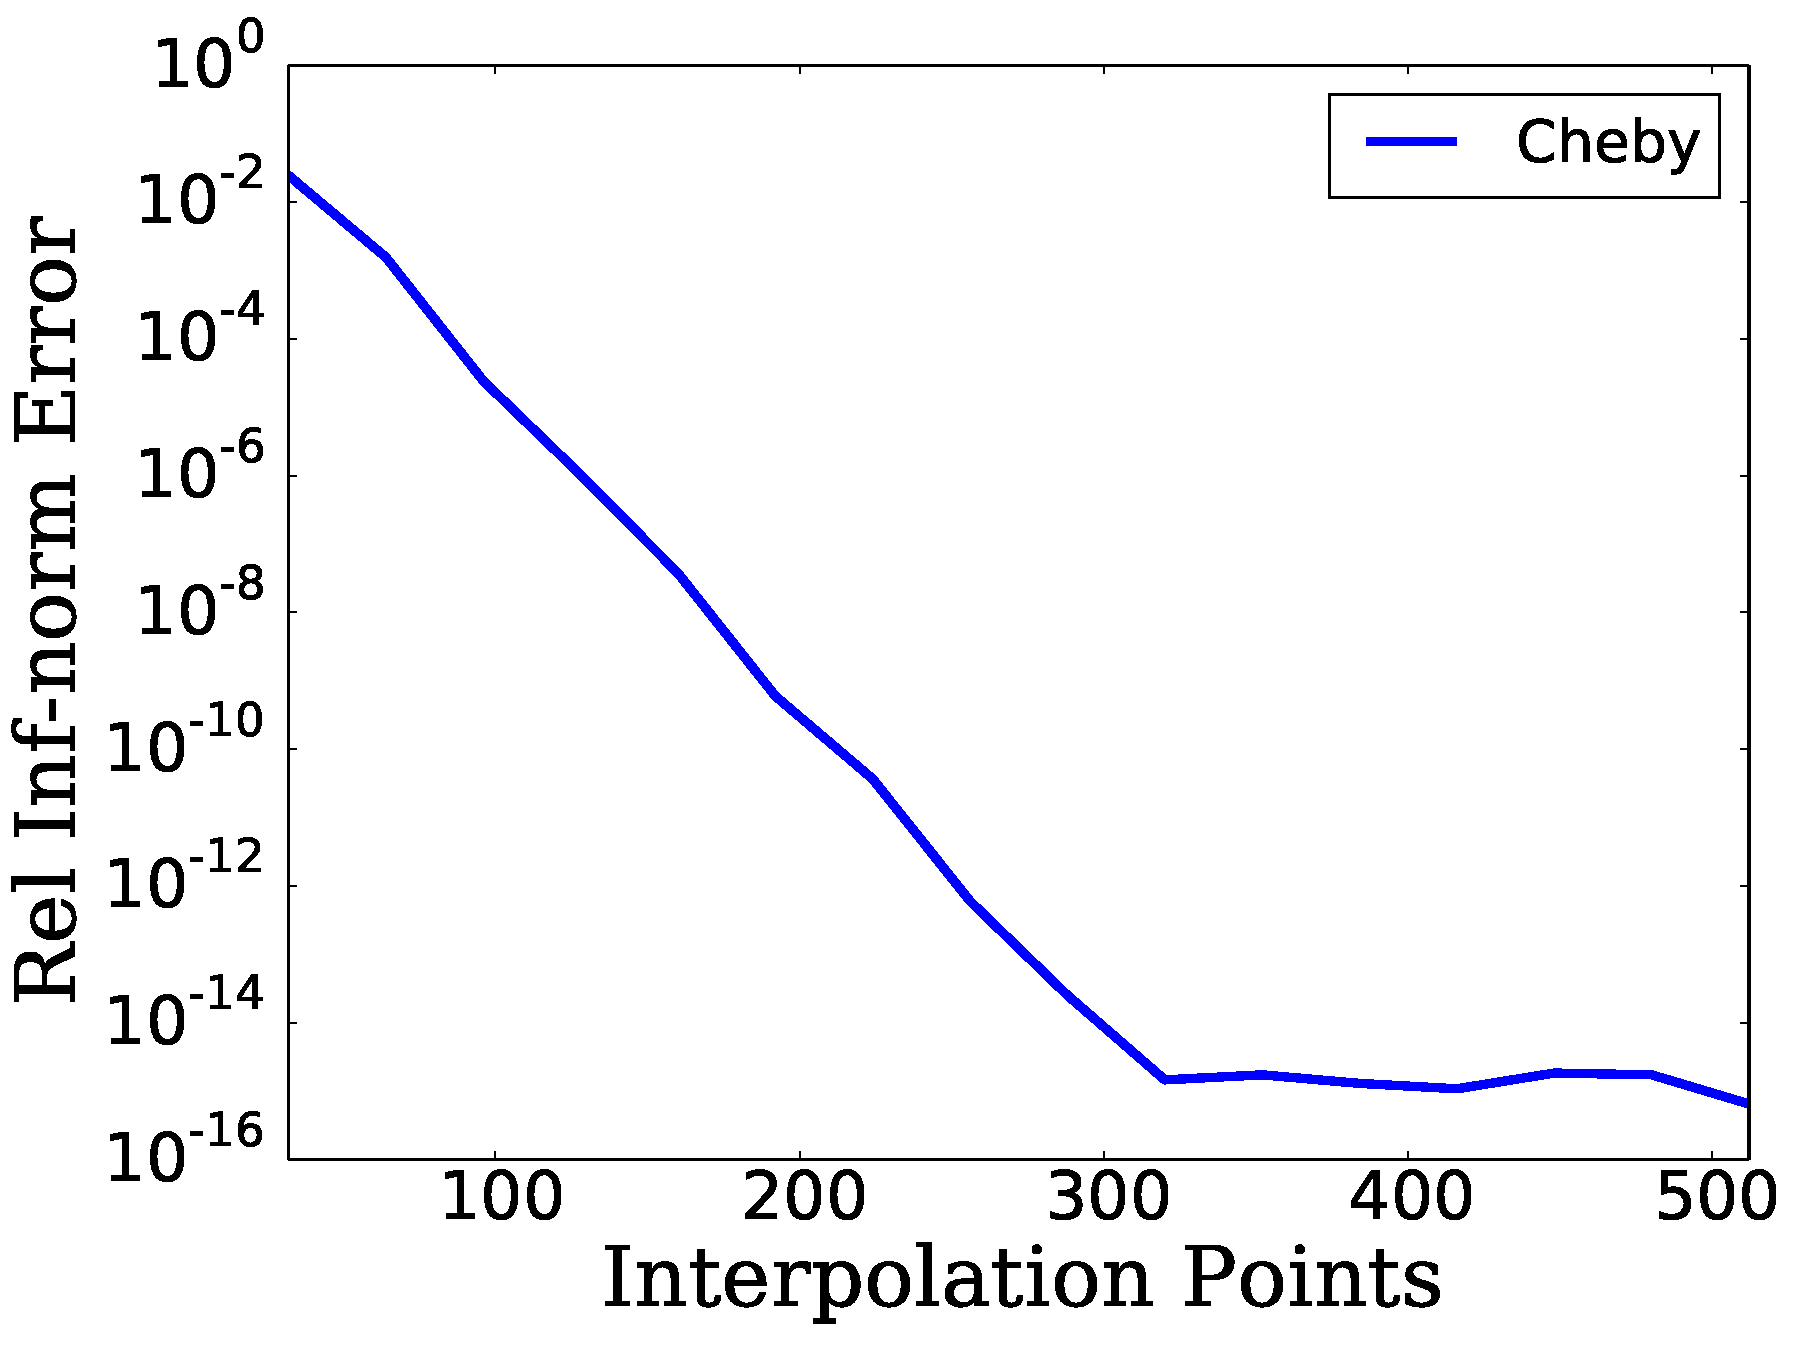
\includegraphics[width=\textwidth]{plots/cheby_1d_smooth_R_100.pdf}
    \caption{$R=100$}
    \end{subfigure}

\caption[Smooth Interpolation Comparison: 1D Runge Function]{
MSN interpolation and Chebyshev interpolation results of the
1D Runge function $g_{25}$ and $g_{100}$ for various $s$ values.
}
\label{fig:smooth_comparison_1d_runge}
\end{figure}





\subsection{Birkhoff Interpolation Comparison}

We now look at a Birkhoff interpolation problem for an approximation $p$:
%
\begin{align}
    p'(z_{k}^{n}) &= g_{R}'(z_{k}^{n}), \quad k\in\braces{1,\cdots,n}
        \nonumber\\
    p(-1) &= g_{R}(-1) \nonumber\\
    p(1) &= g_{R}(1).
\end{align}
%
Fast MSN methods exist and we compare against Chebyshev interpolation.
In particular, the system
%
\begin{equation}
    \begin{bmatrix} UWD \\ A \end{bmatrix} a
        = \begin{bmatrix} UC^{-1}f' \\ f \end{bmatrix},
    \label{eq:smooth_birkhoff_system}
\end{equation}
%
where $f'$ holds the derivative information and $f$ holds the
endpoint interpolation, is solved using pivoted QR.
The $UWD$ matrix is truncated so that the entire system is square,
and from our previous work we know $UWD$ is mostly zero.
The standard method for solving linear systems in Julia
is pivoted LU~\cite{julialang}, although there is no noticeable difference
between pivoted QR and pivoted LU (results not shown).
The results for can be seen in
Fig.~\ref{fig:smooth_comparison_1d_runge_birkhoff}.
When solving the square system, it is clear numerical
difficulties are keeping the minimal error around $10^{-14}$.
The error decay of both methods are approximately the same.

Due to the structure of the linear system, it would be possible
to implement a similar fast solver for the square system.

% Print results for comparing MSN with 2D Runge function

\begin{figure}[p]
    \centering
    \begin{subfigure}{0.45\textwidth}
    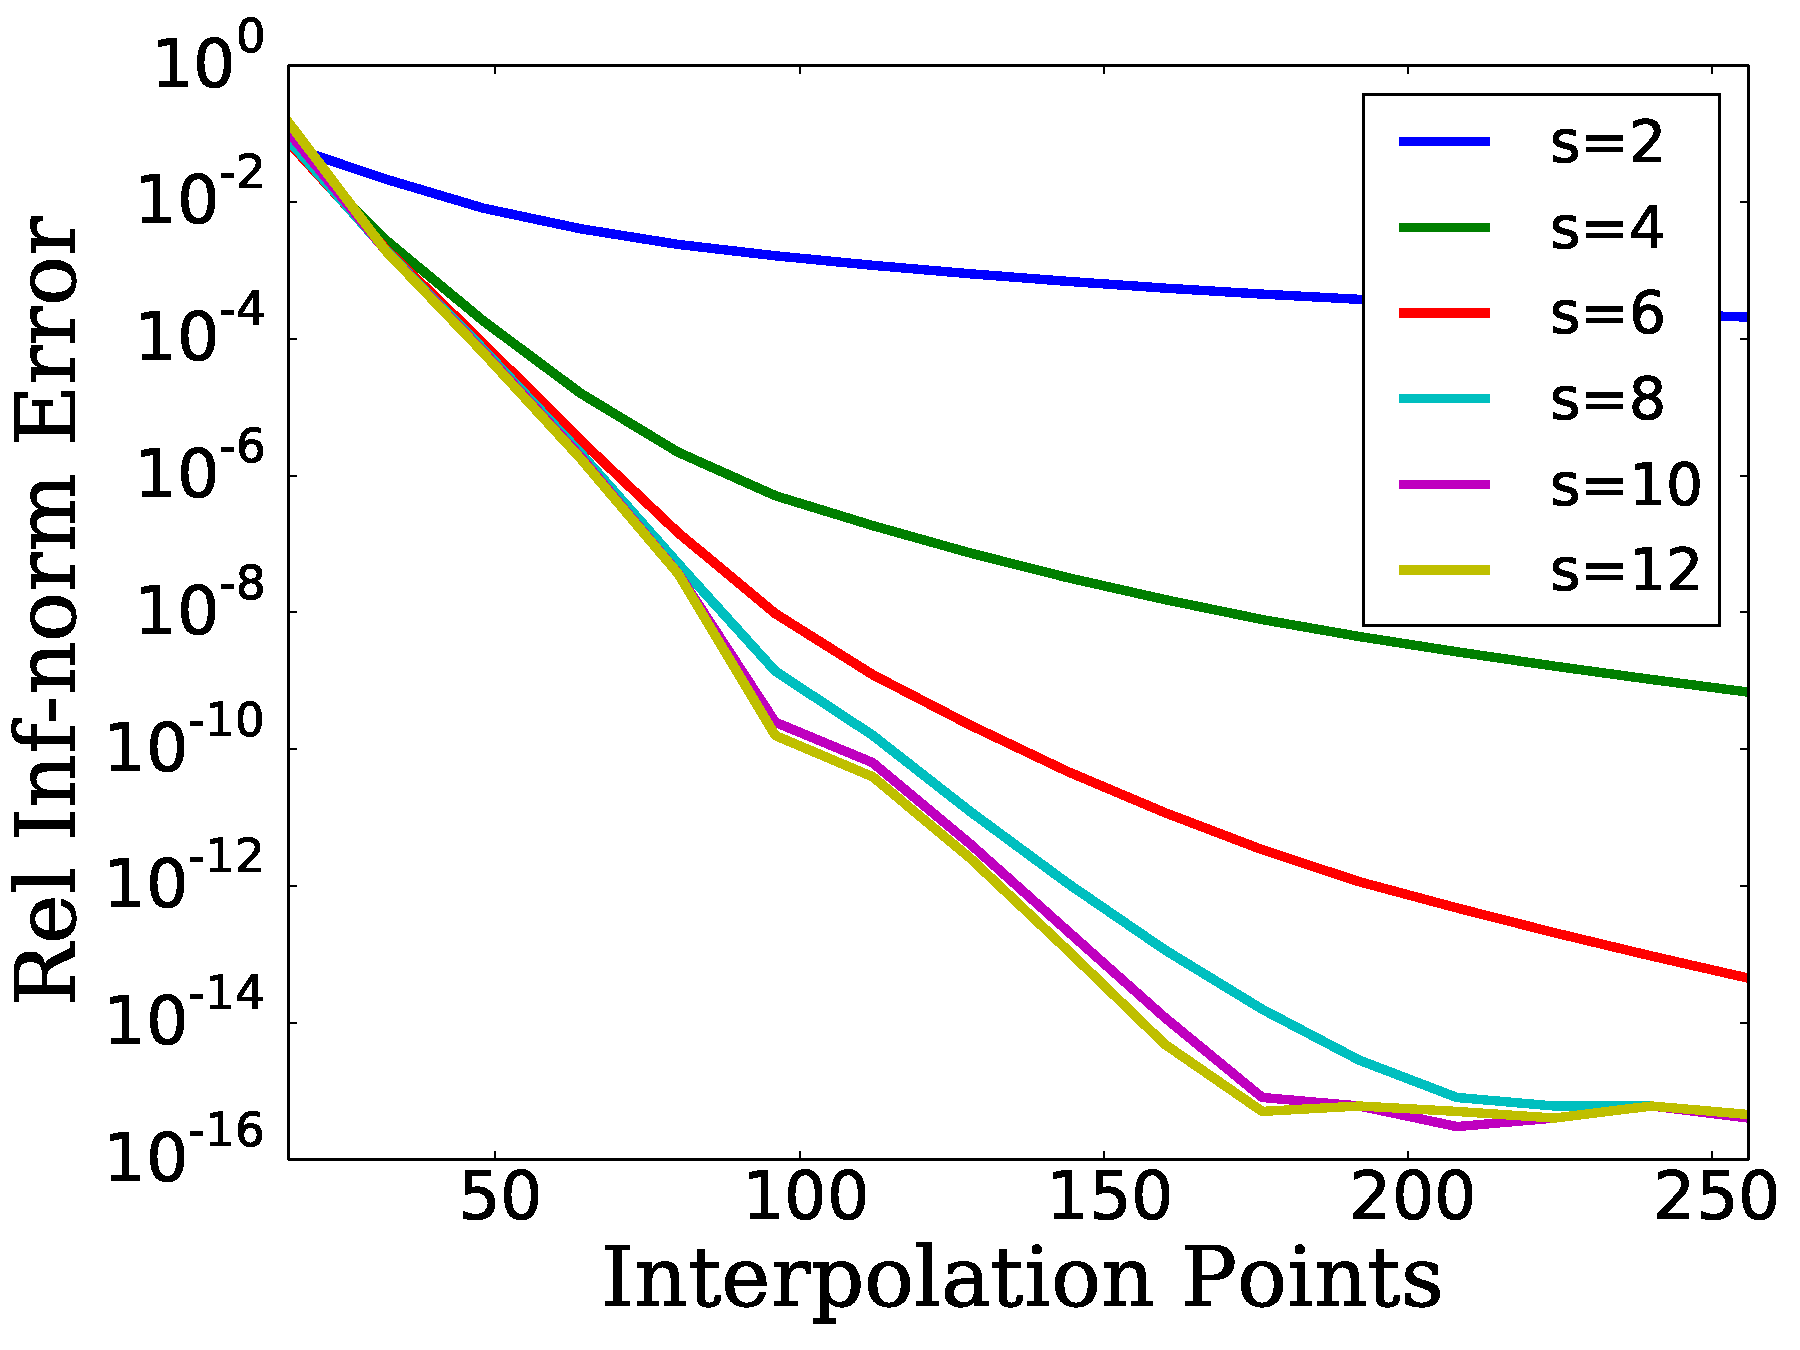
\includegraphics[width=\textwidth]{plots/msn_1d_birkhoff_smooth_R_25.pdf}
    \caption{$R=25$}
    \end{subfigure}
    \begin{subfigure}{0.45\textwidth}
    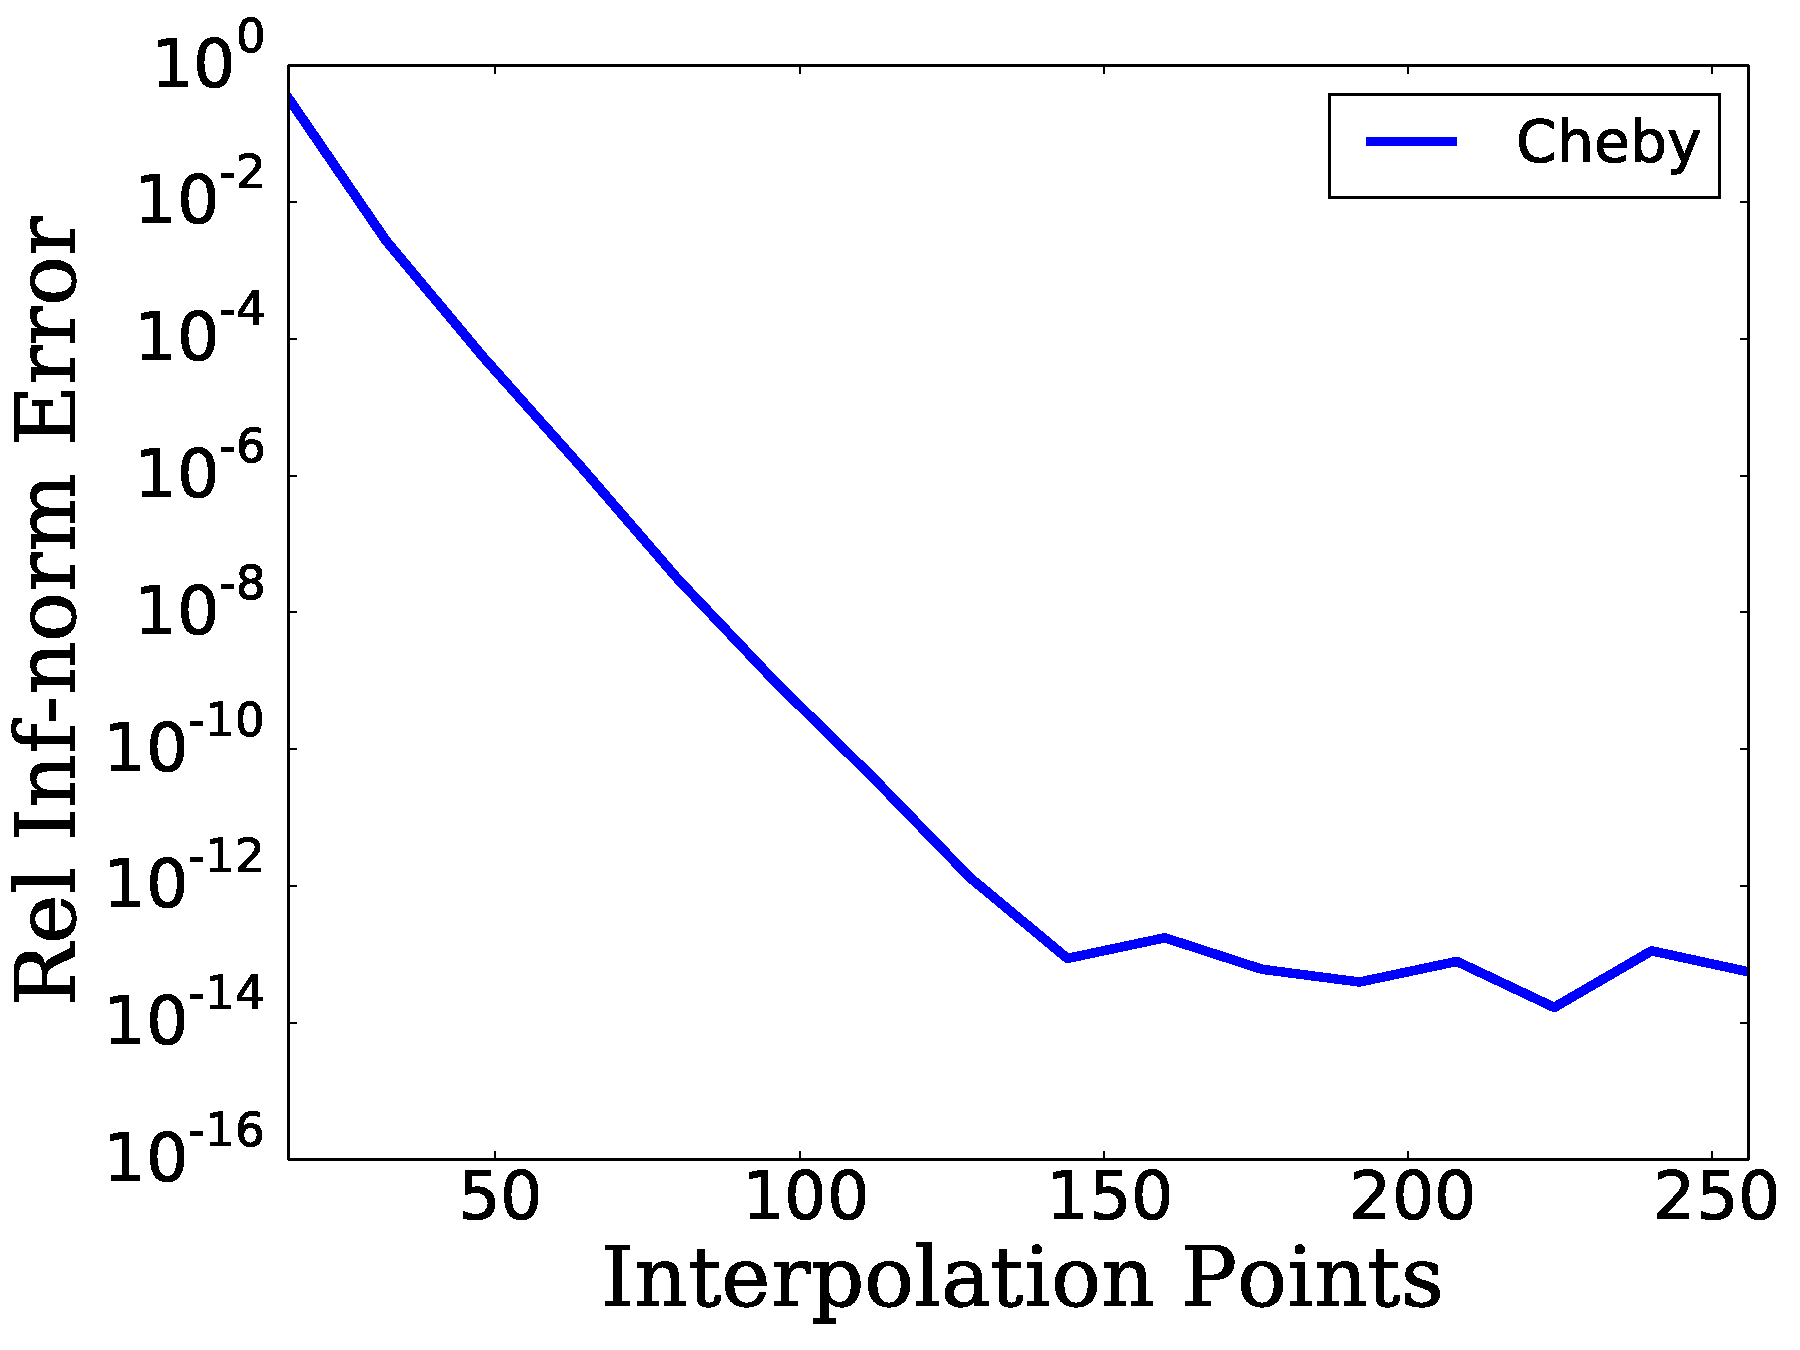
\includegraphics[width=\textwidth]{plots/cheby_1d_birkhoff_smooth_R_25.pdf}
    \caption{$R=25$}
    \end{subfigure}

    \begin{subfigure}{0.45\textwidth}
    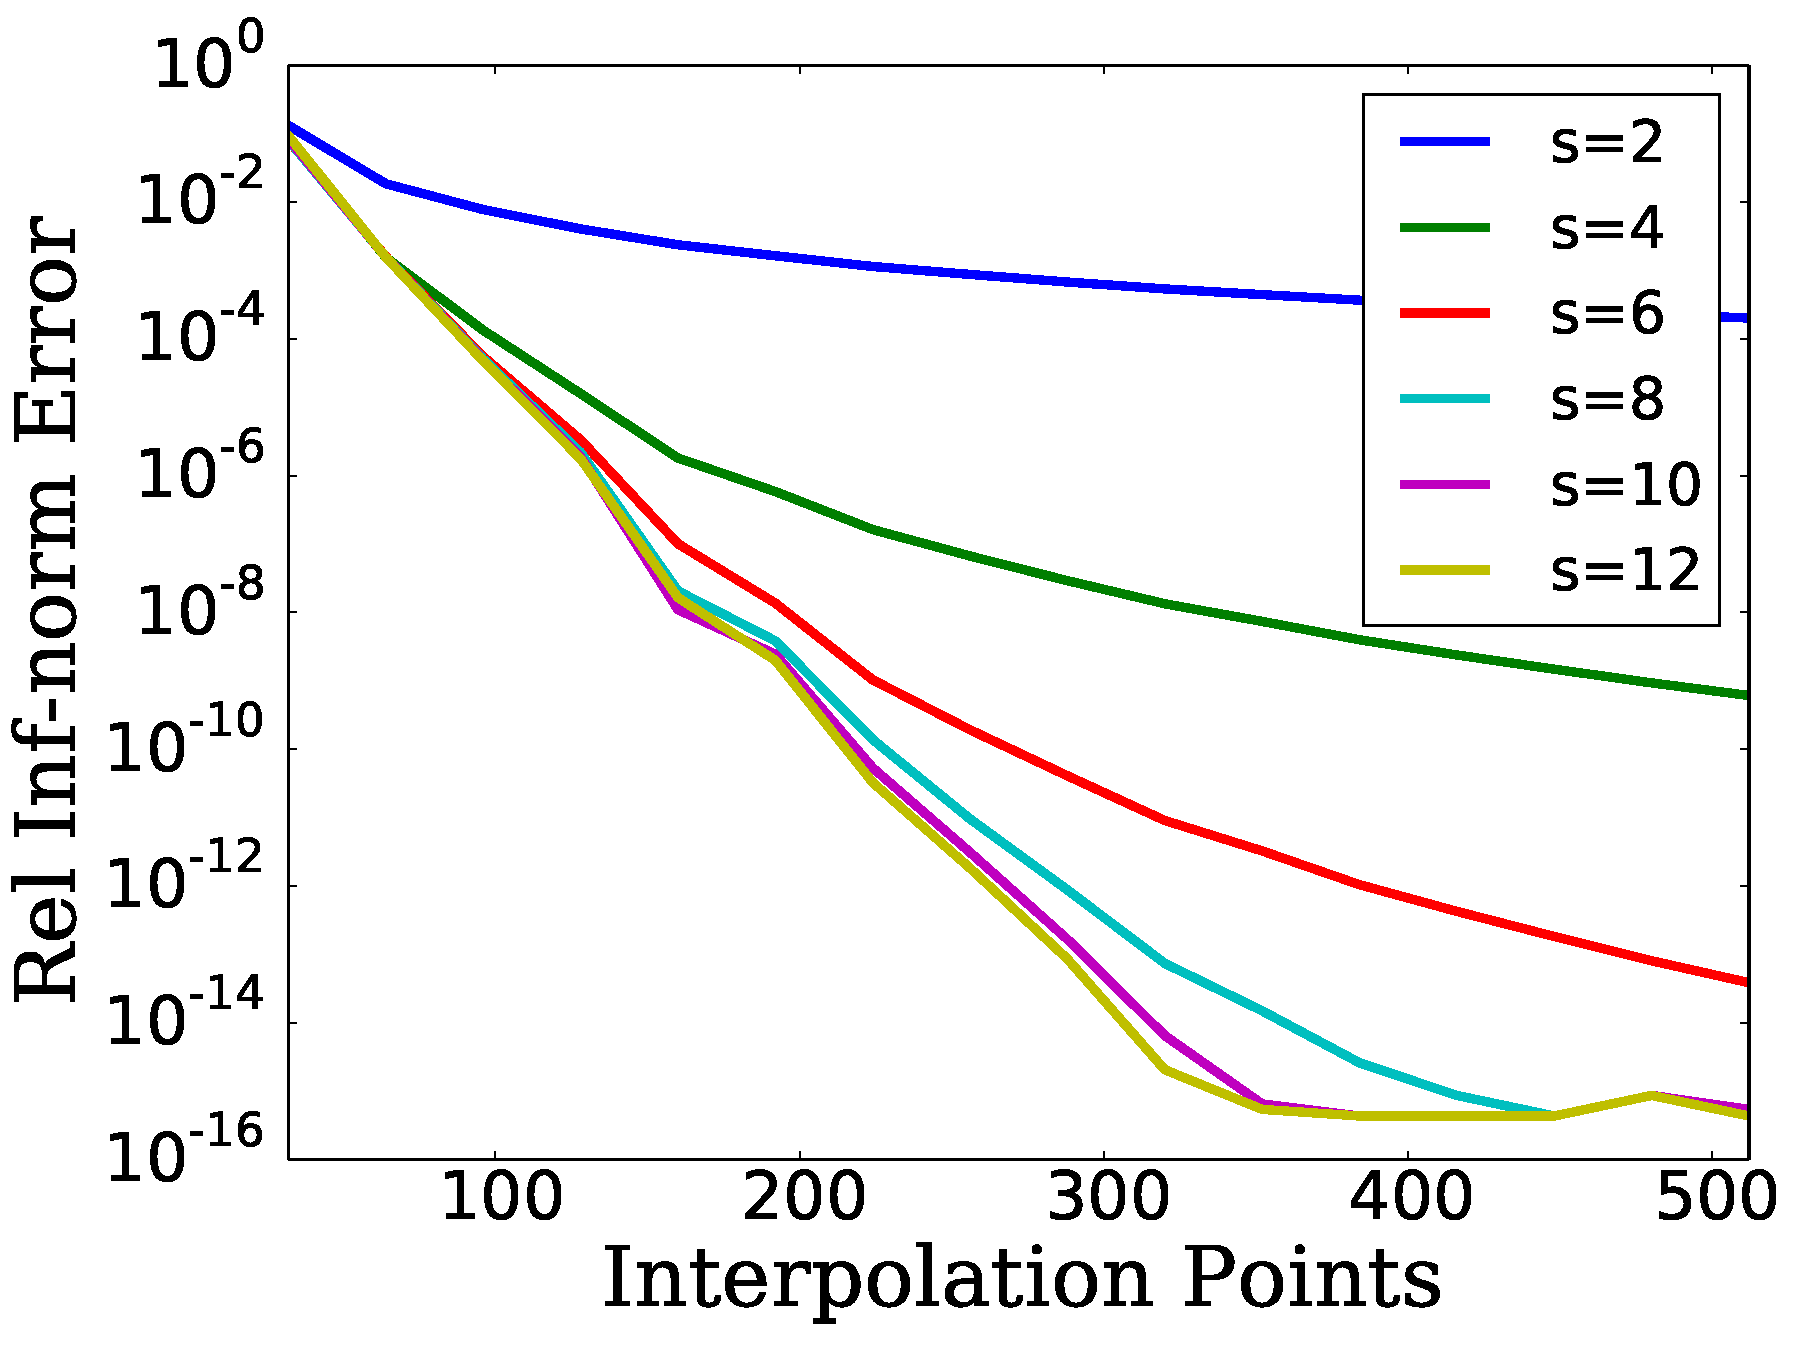
\includegraphics[width=\textwidth]{plots/msn_1d_birkhoff_smooth_R_100.pdf}
    \caption{$R=100$}
    \end{subfigure}
    \begin{subfigure}{0.45\textwidth}
    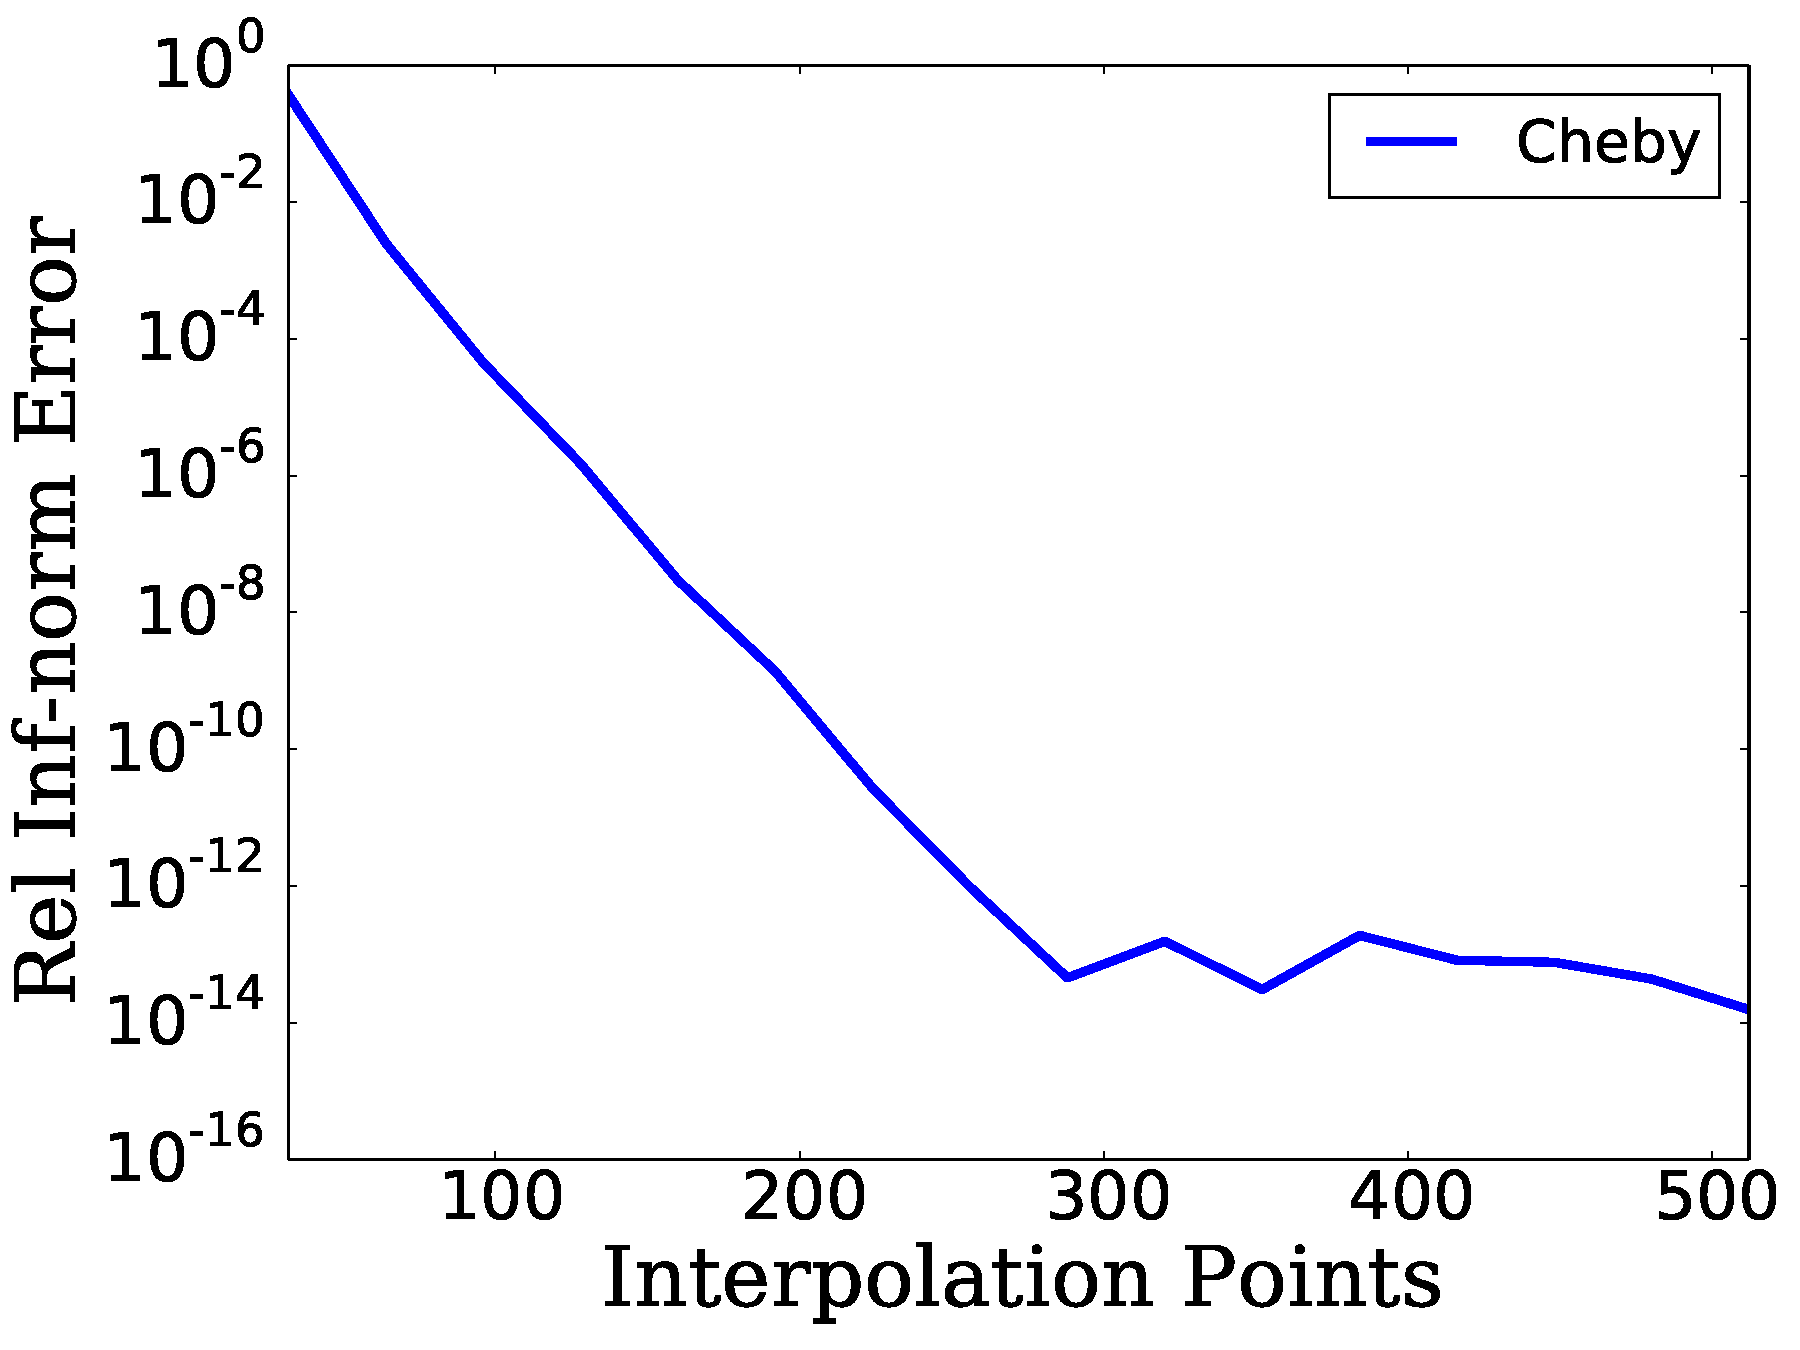
\includegraphics[width=\textwidth]{plots/cheby_1d_birkhoff_smooth_R_100.pdf}
    \caption{$R=100$}
    \end{subfigure}

\caption[Smooth Birkhoff Interpolation Comparison: 1D Runge Function]{
MSN Birkhoff interpolation and Chebyshev interpolation results
of the 1D Runge function $g_{25}$ and $g_{100}$ for various $s$ values.
}
\label{fig:smooth_comparison_1d_runge_birkhoff}
\end{figure}






\section{Results for Fast MSN Interpolation in 2D for Smooth Functions}
\label{sec:vs_I_2d}

We now turn our attention to the more difficult challenge
of interpolating the 2D function $f_{R}$.
For $R=25$, we have results in single and double precision presented
in Fig.~\ref{fig:smooth_comparison_2d_runge_25}.
For $R=100$, we have results in single and double precision presented
in Fig.~\ref{fig:smooth_comparison_2d_runge_100}.
From these examples, we see that, as before,
MSN interpolation has the same level of approximation as Chebyshev
interpolation for large $s$ values.

% Print results for comparing MSN with 2D Runge function

\begin{figure}[p]
    \centering
    \begin{subfigure}{0.45\textwidth}
    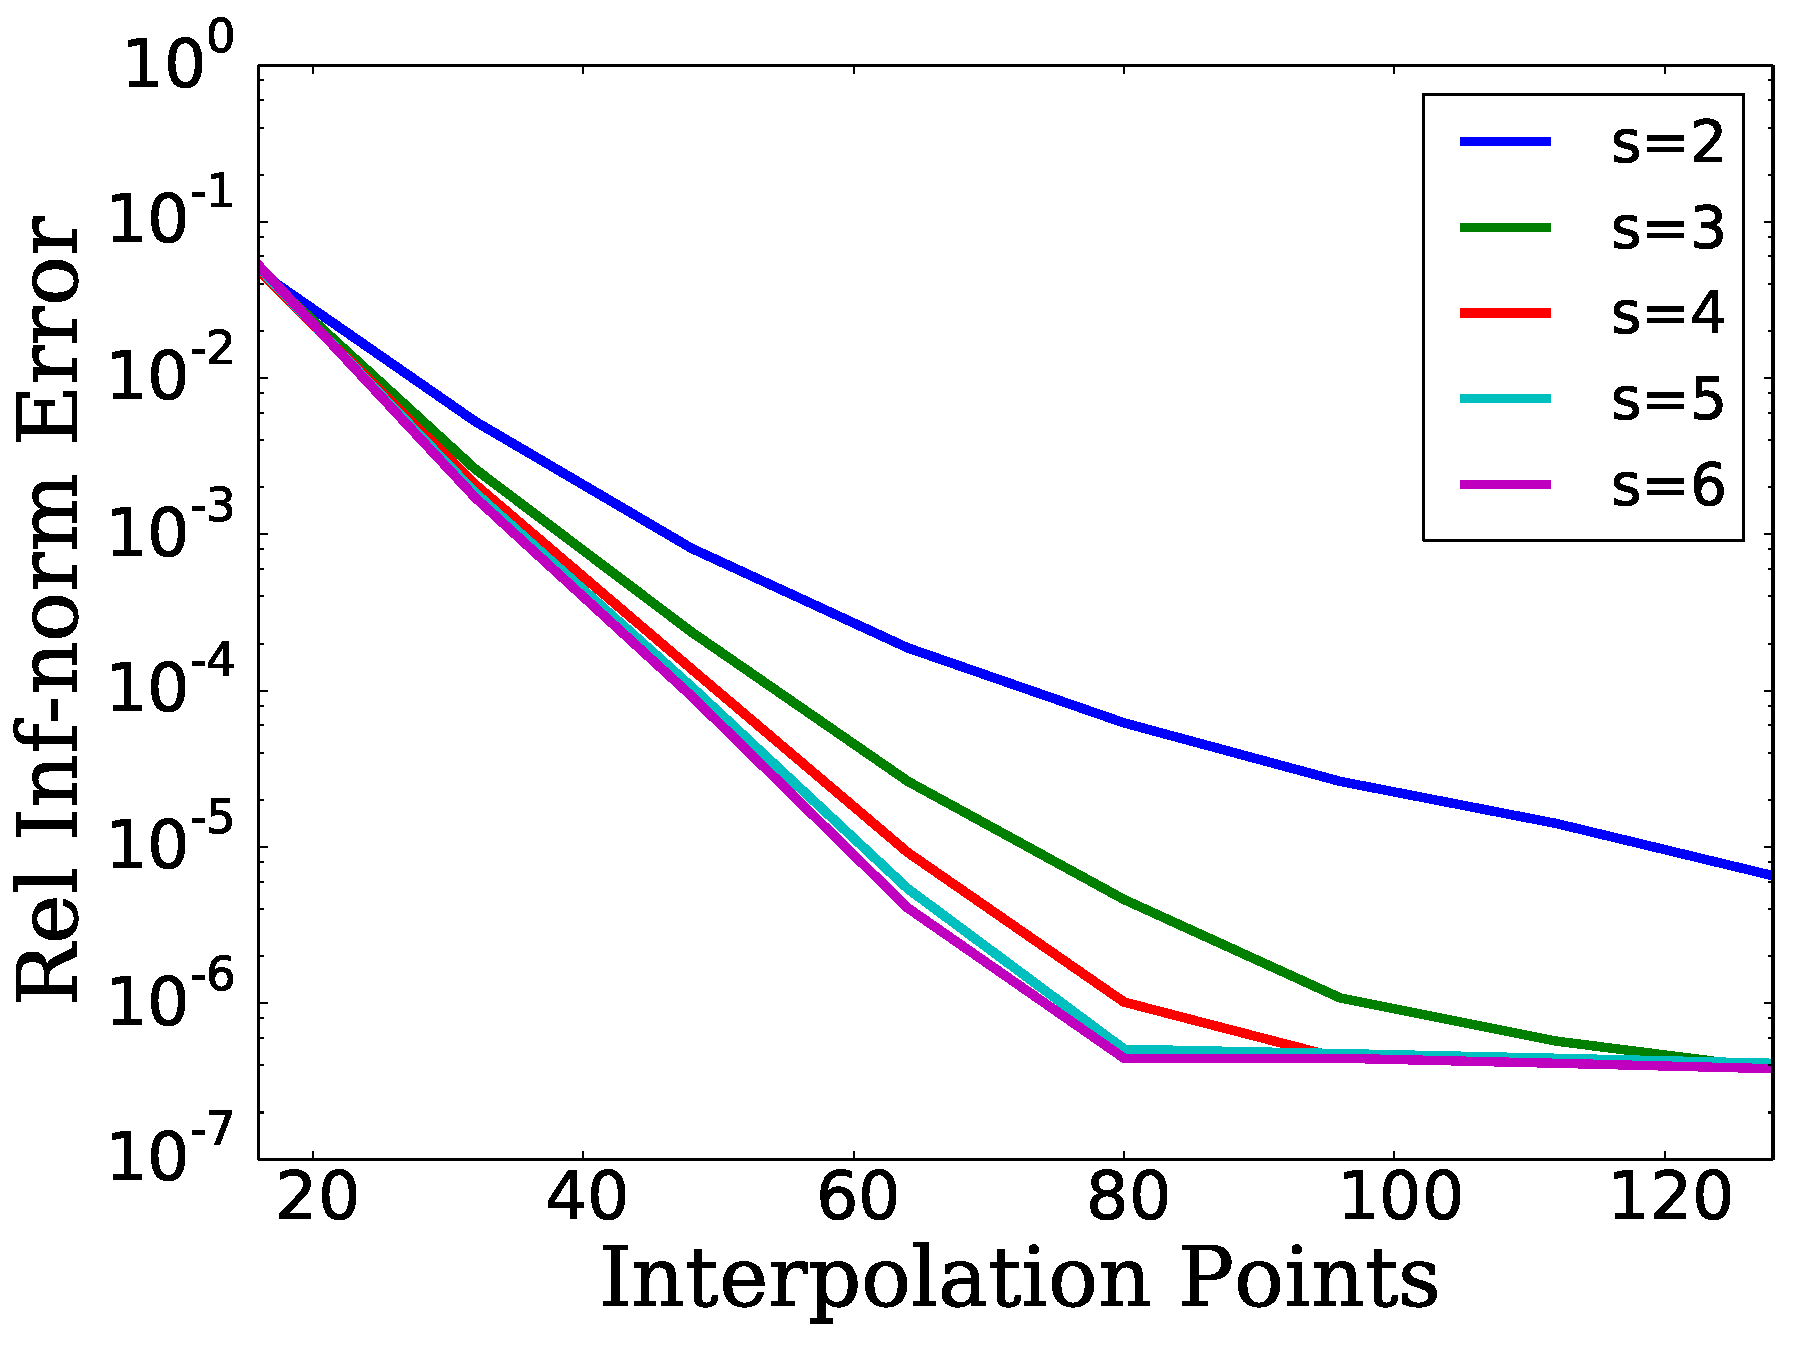
\includegraphics[width=\textwidth]{plots/msn_2n_fast_smooth_R_25_single.pdf}
    \caption{Single Precision}
    \end{subfigure}
    \begin{subfigure}{0.45\textwidth}
    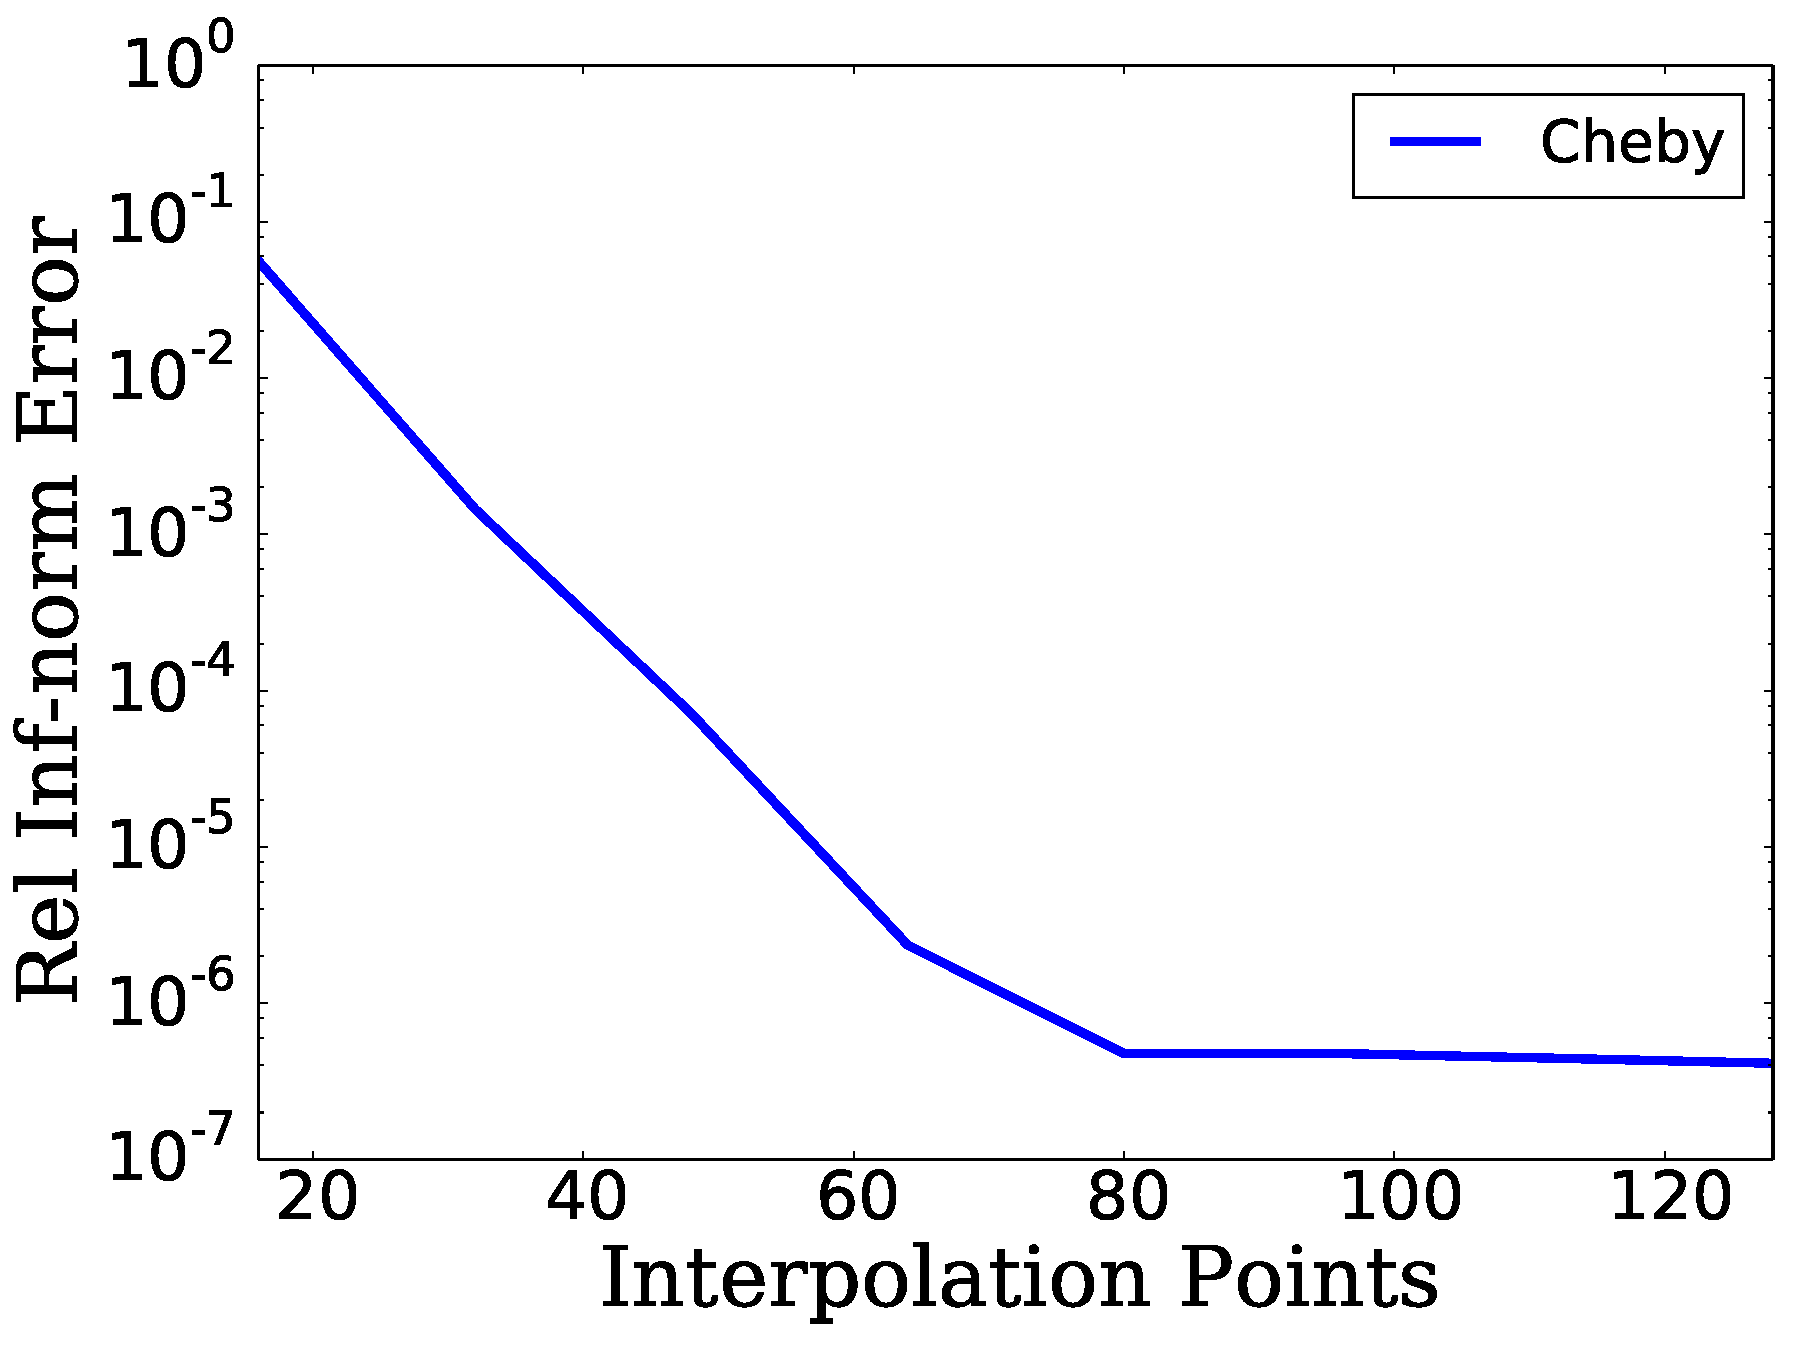
\includegraphics[width=\textwidth]{plots/cheby_interp_smooth_R_25_single.pdf}
    \caption{Single Precision}
    \end{subfigure}

    \begin{subfigure}{0.45\textwidth}
    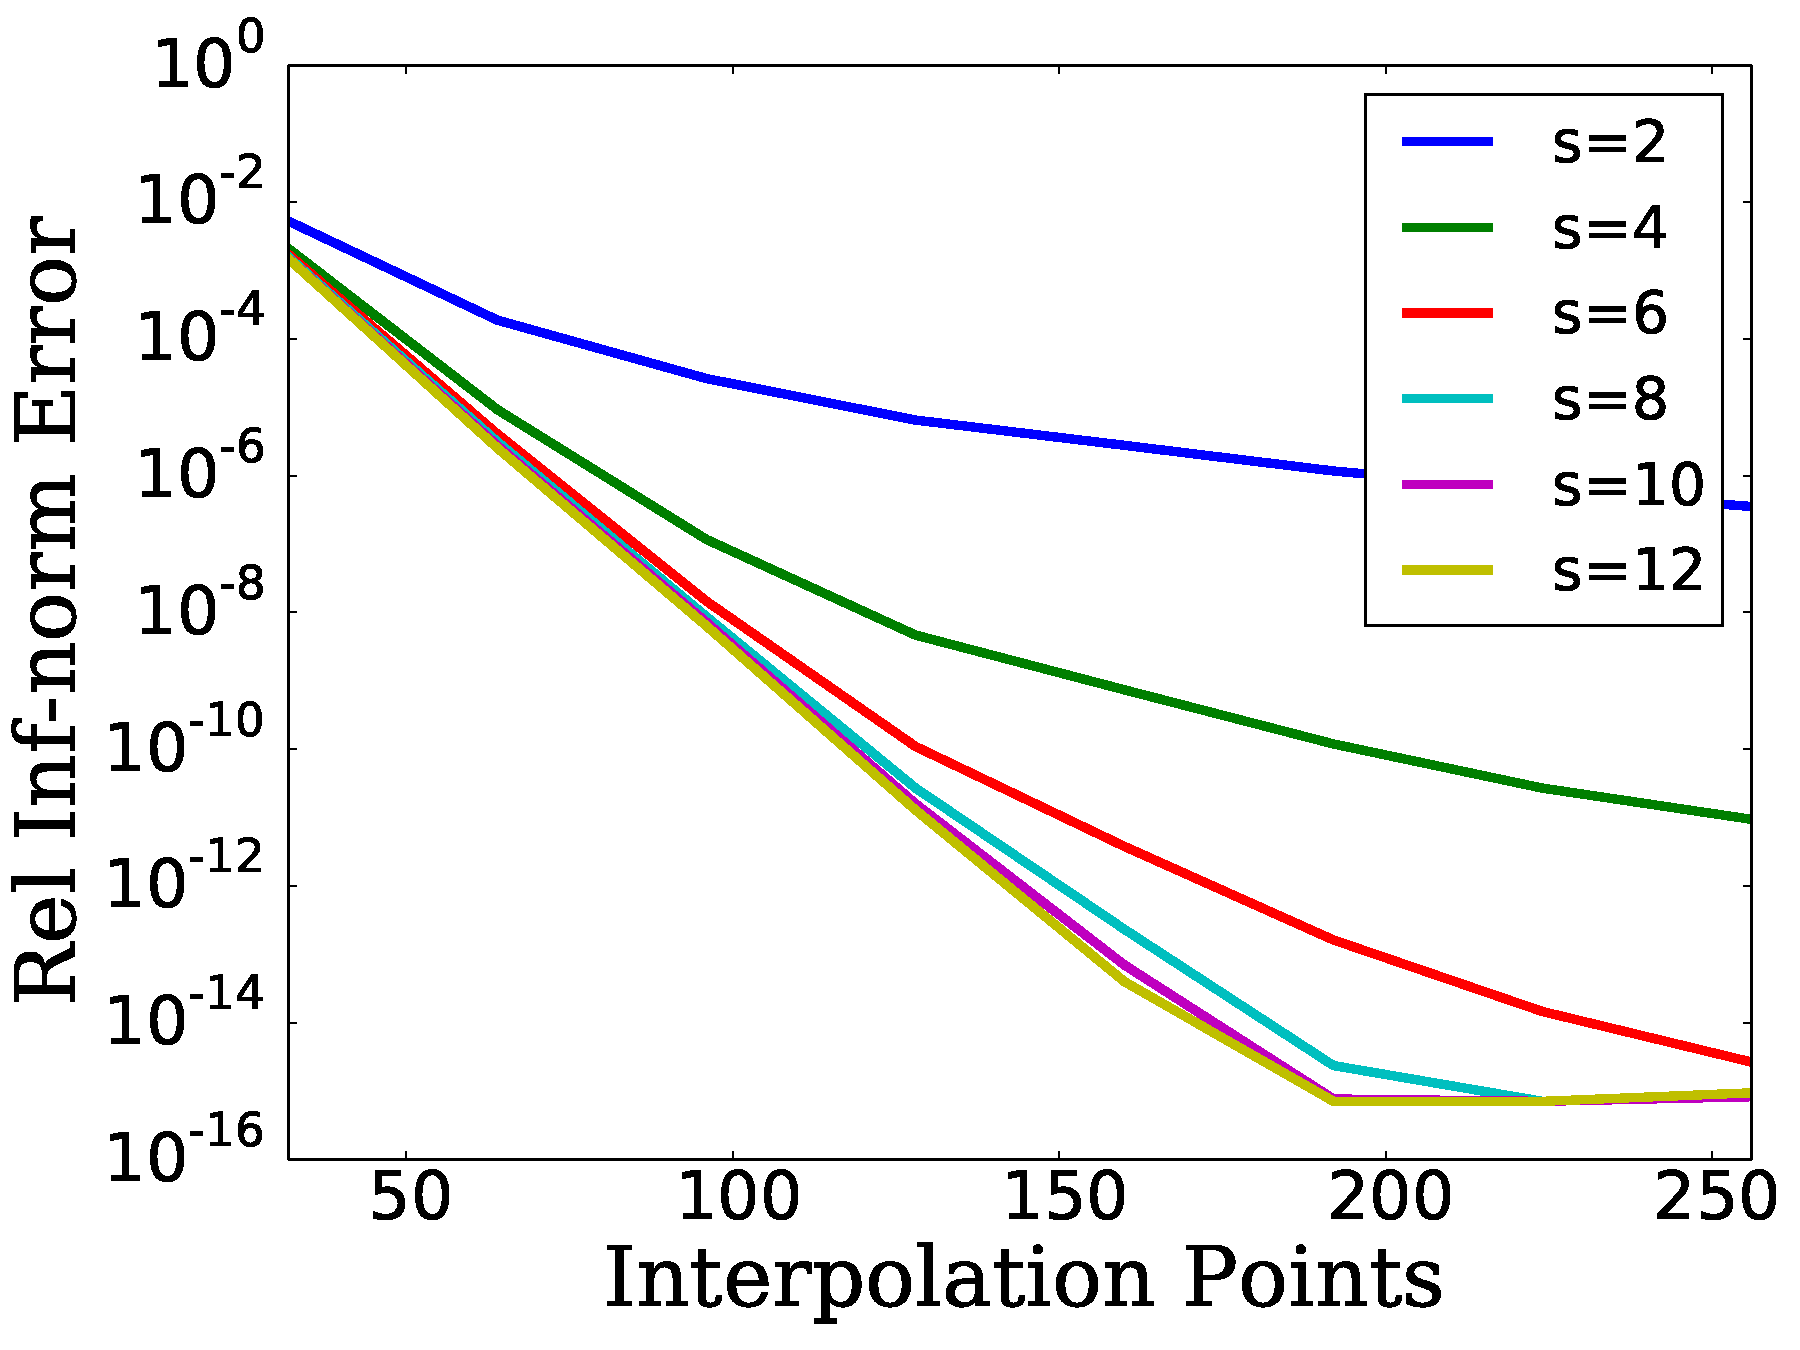
\includegraphics[width=\textwidth]{plots/msn_2n_fast_smooth_R_25_double.pdf}
    \caption{Double Precision}
    \end{subfigure}
    \begin{subfigure}{0.45\textwidth}
    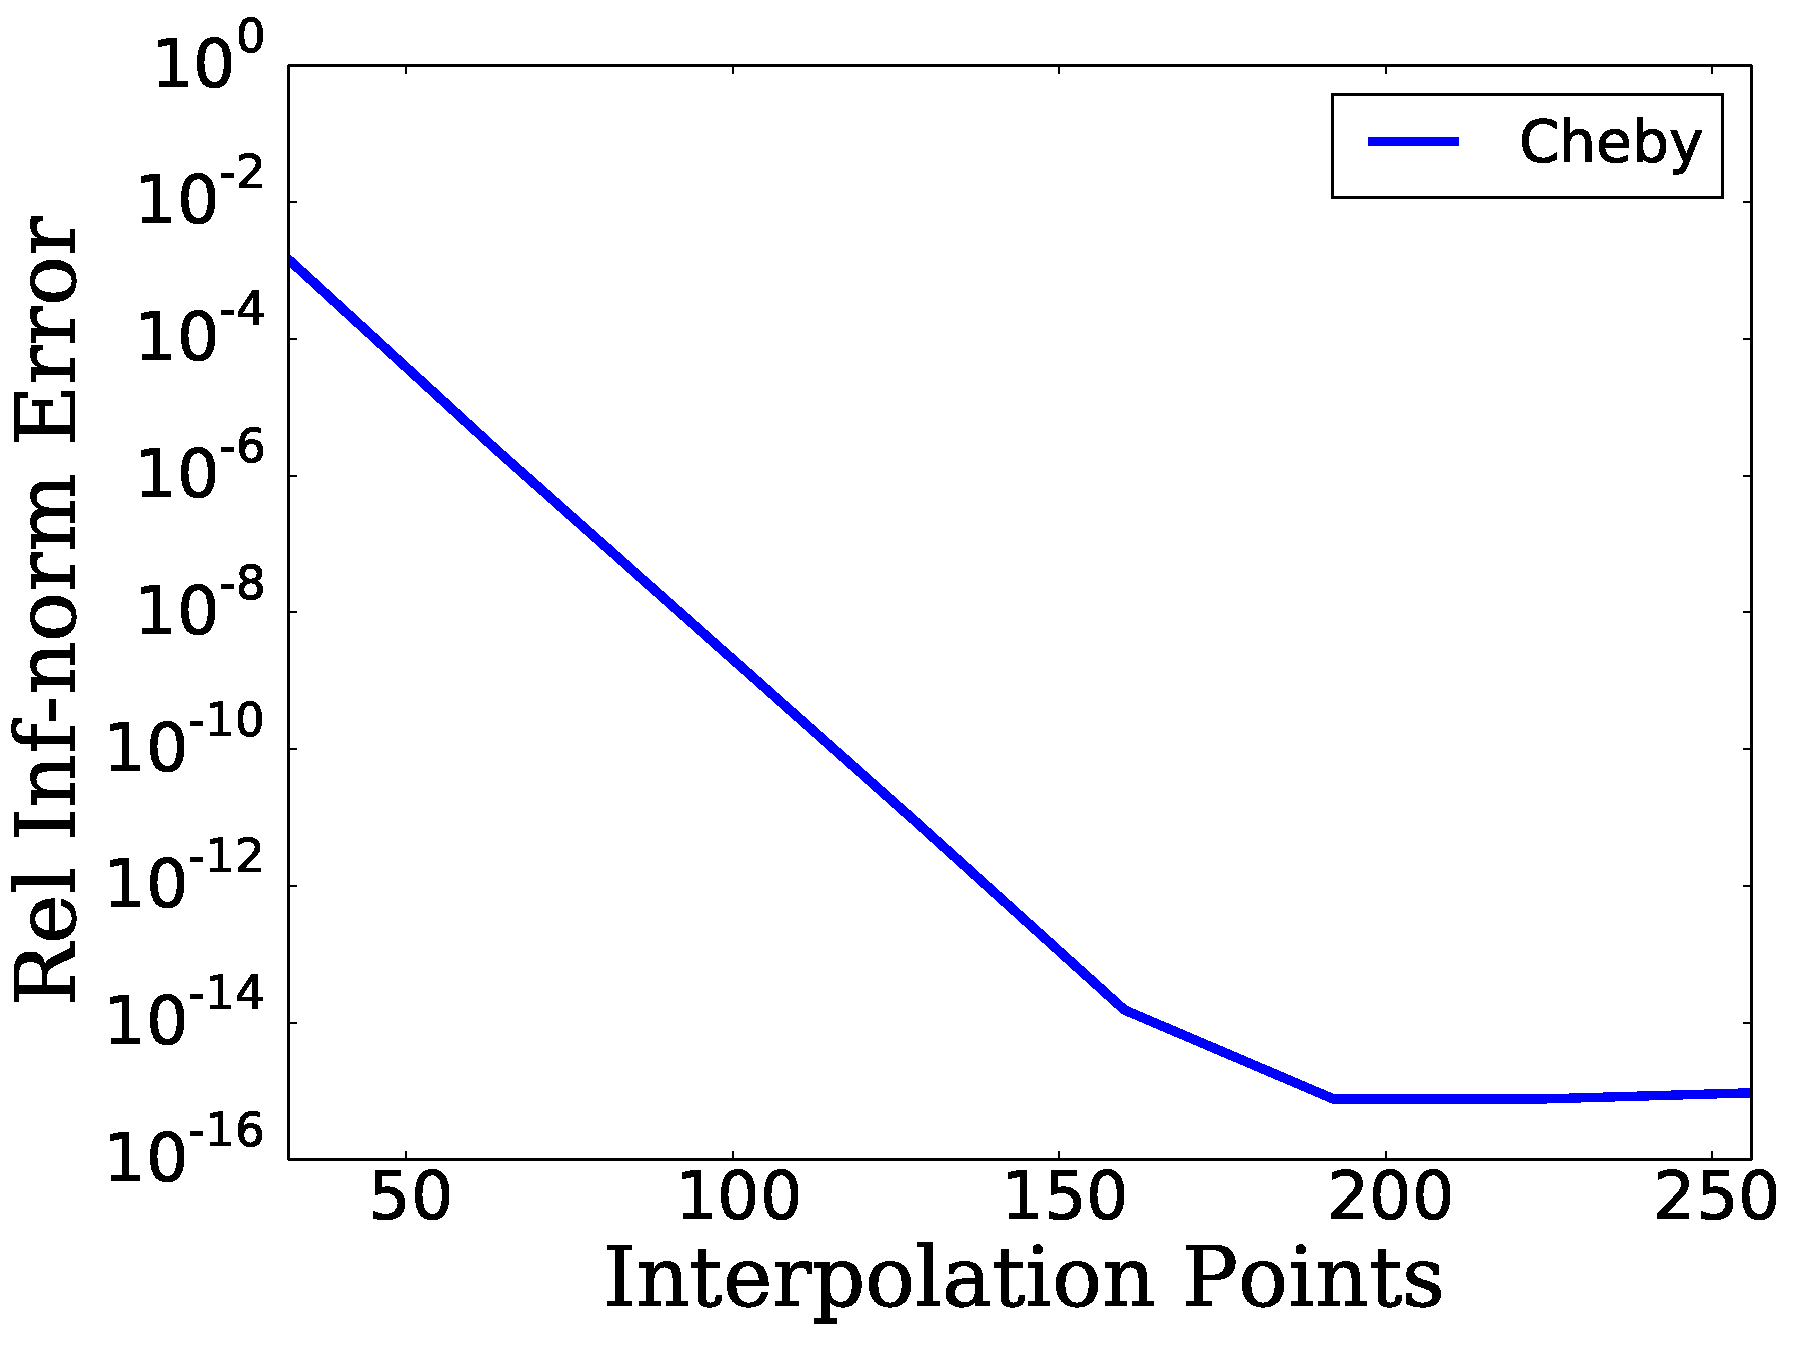
\includegraphics[width=\textwidth]{plots/cheby_interp_smooth_R_25_double.pdf}
    \caption{Double Precision}
    \end{subfigure}
\caption[Smooth Interpolation Comparison: 2D Runge Function $R=25$]{
MSN interpolation and Chebyshev interpolation results
of the 2D Runge function $f_{25}$ for various $s$ values.
Here, $n$ interpolation points refers to interpolation on the $n\times n$
tensor grid of Chebyshev points.
}
\label{fig:smooth_comparison_2d_runge_25}
\end{figure}




% Print results for comparing MSN with 2D Runge function

\begin{figure}[p]
    \centering
    \begin{subfigure}{0.45\textwidth}
    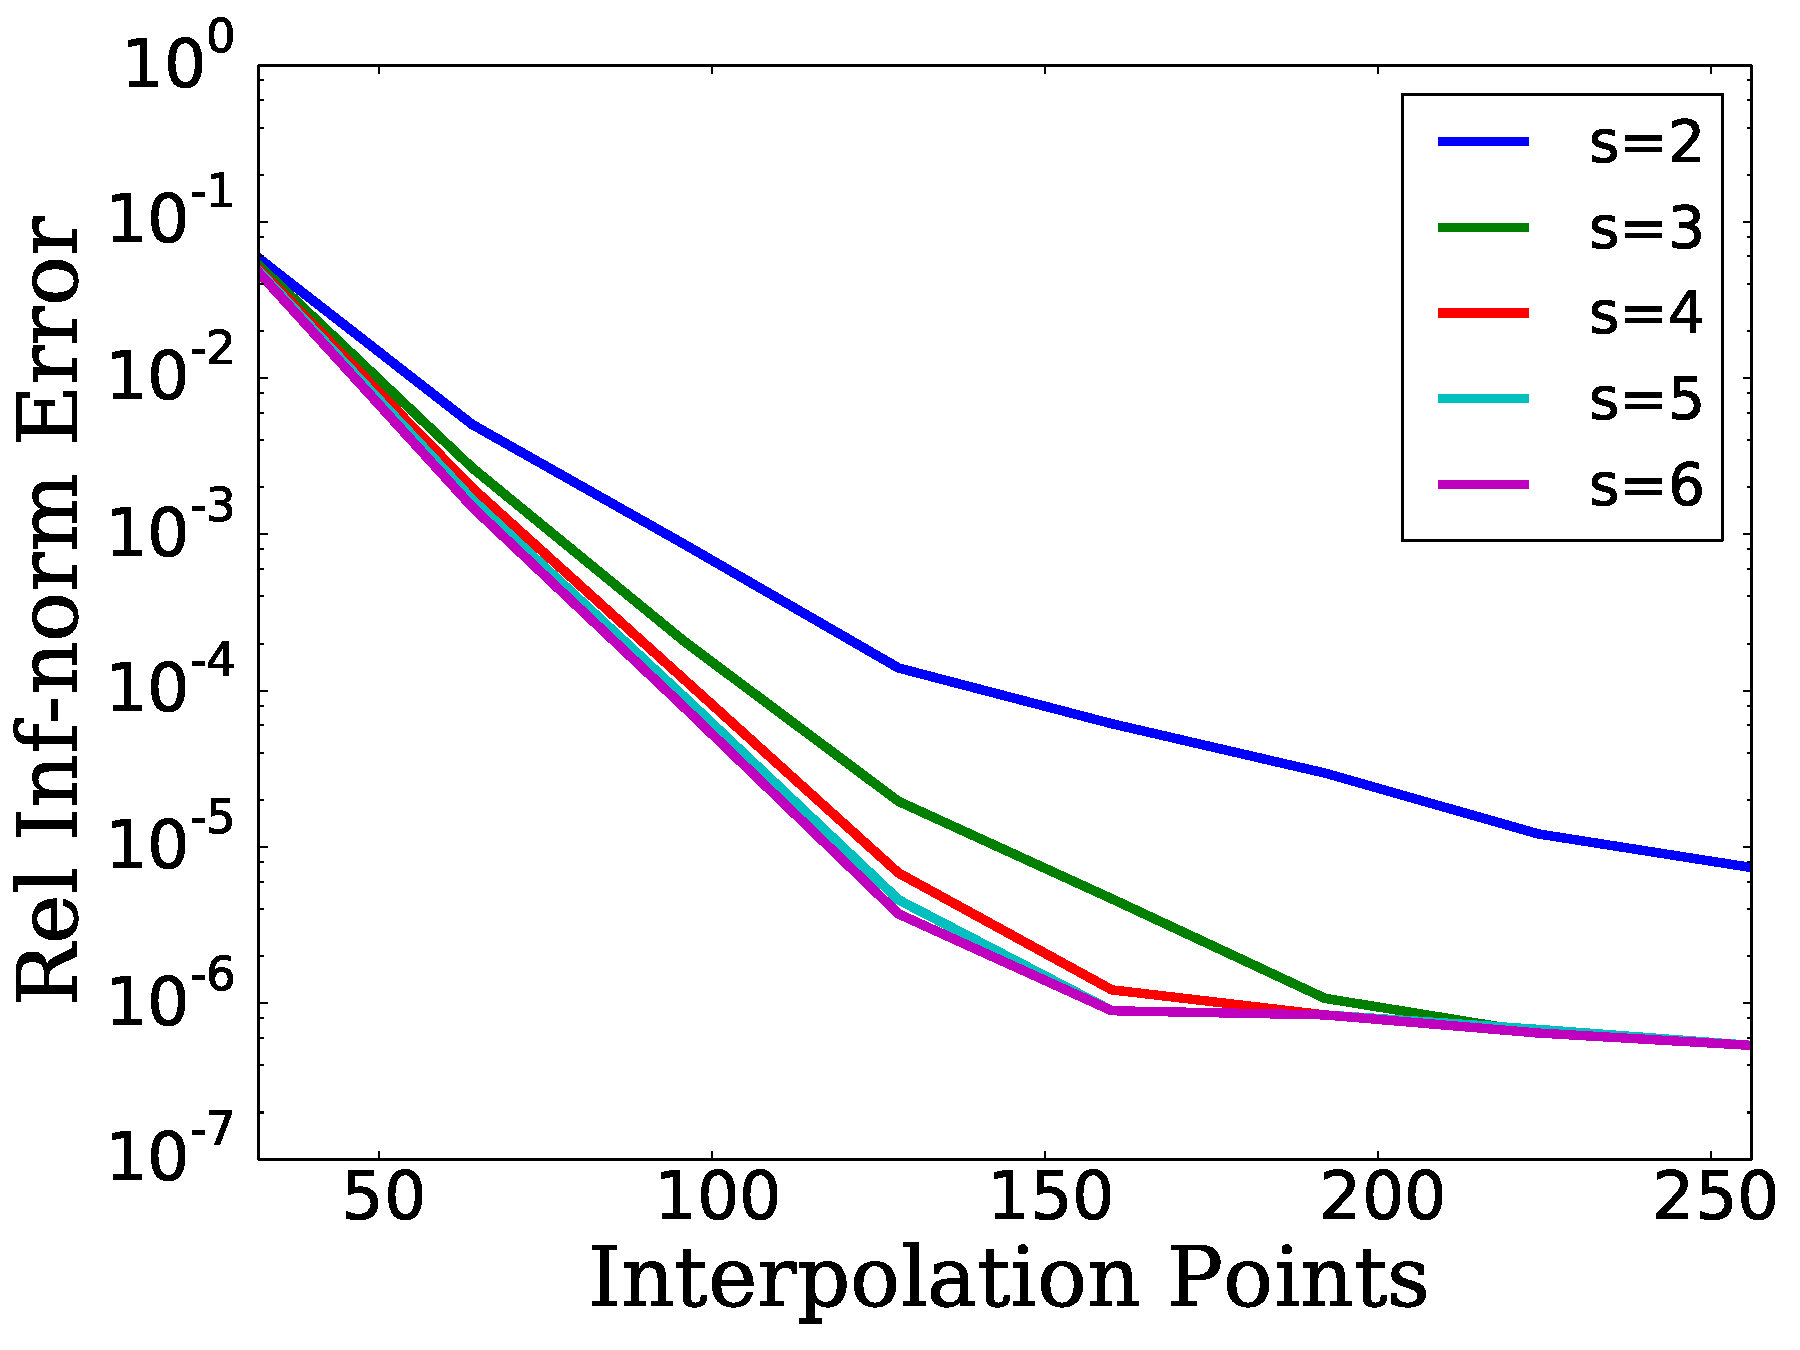
\includegraphics[width=\textwidth]{plots/msn_2n_fast_smooth_R_100_single.pdf}
    \caption{Single Precision}
    \end{subfigure}
    \begin{subfigure}{0.45\textwidth}
    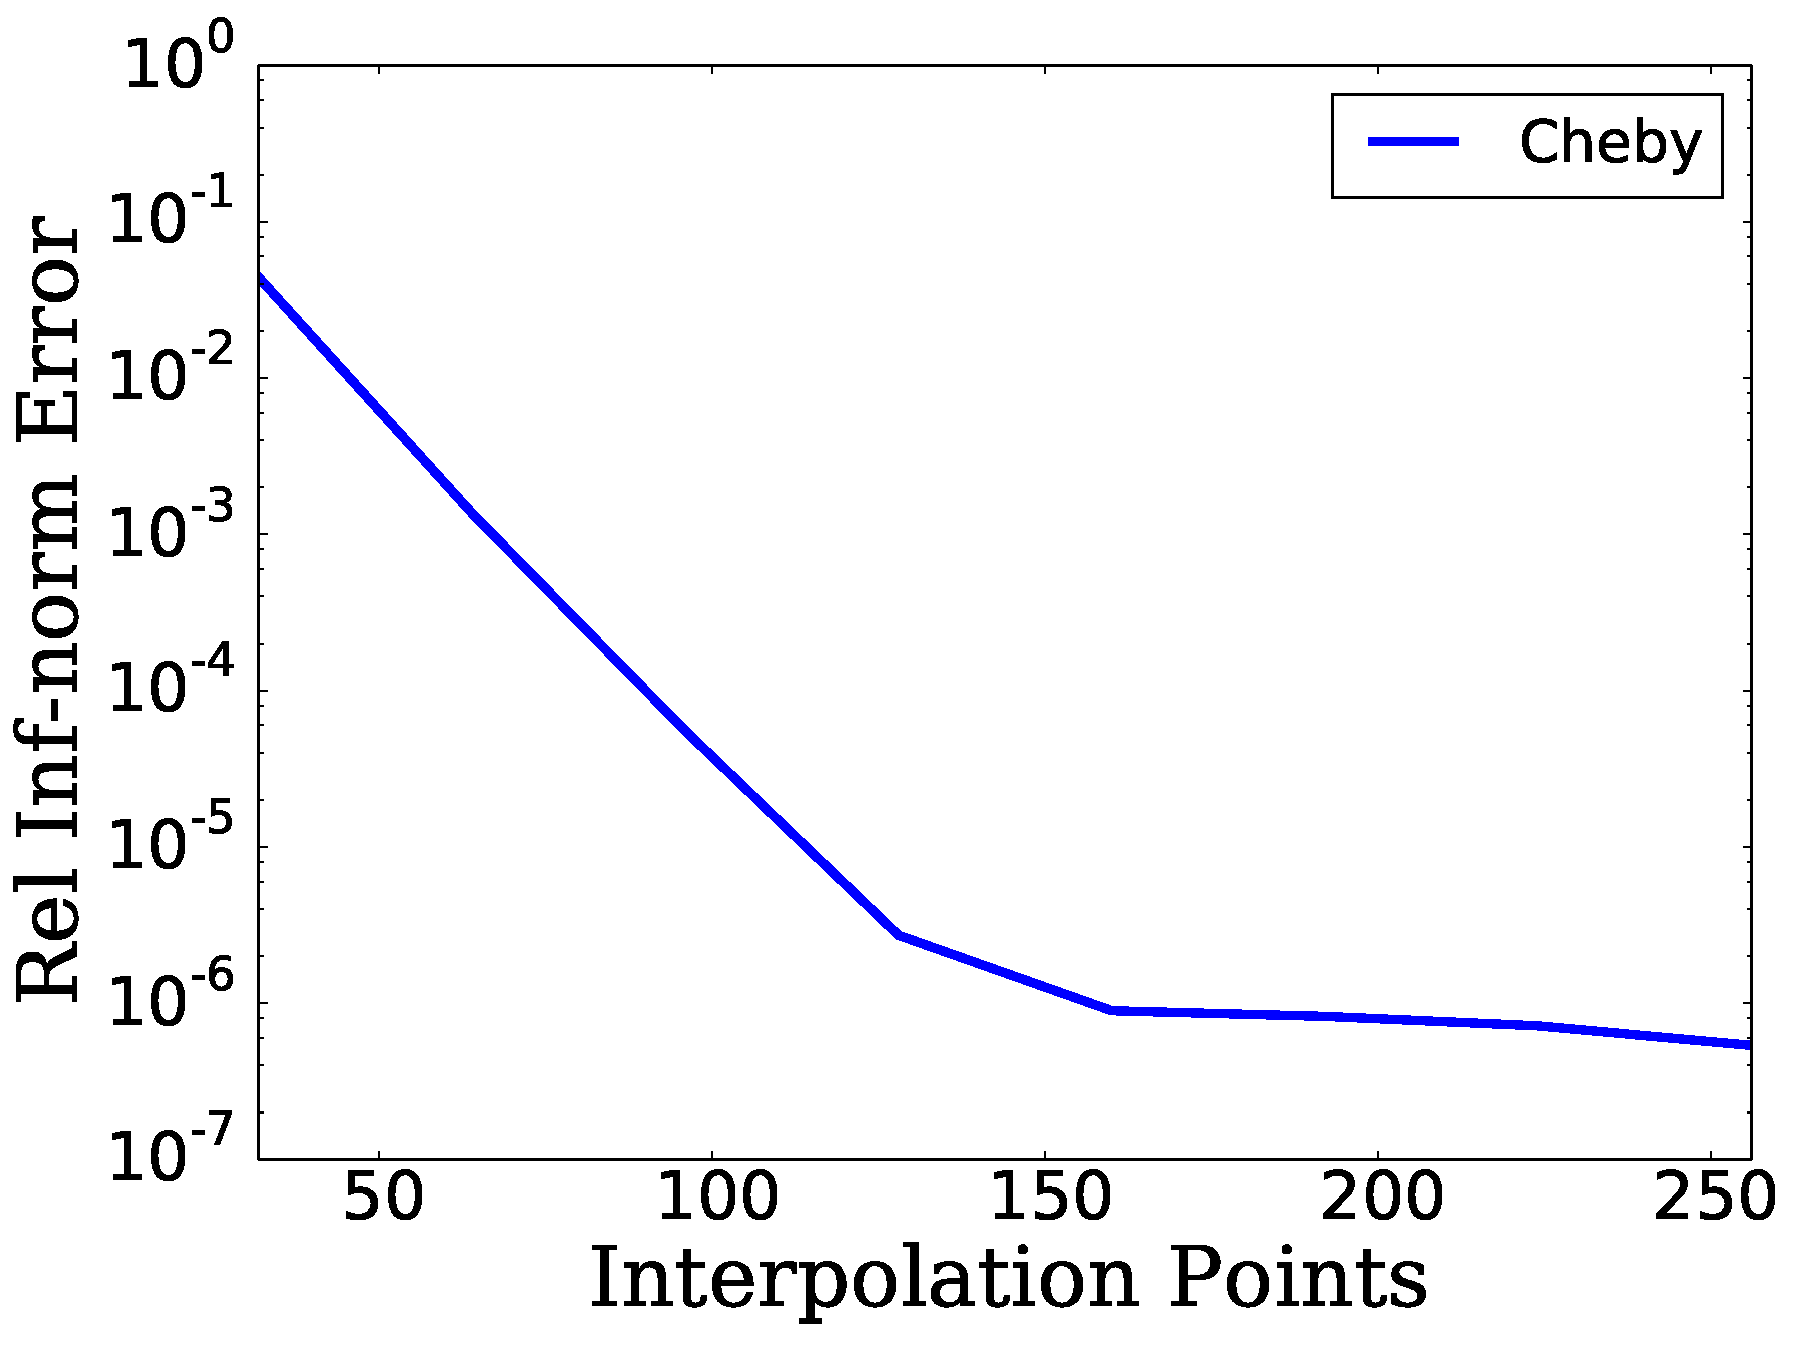
\includegraphics[width=\textwidth]{plots/cheby_interp_smooth_R_100_single.pdf}
    \caption{Single Precision}
    \end{subfigure}

    \begin{subfigure}{0.45\textwidth}
    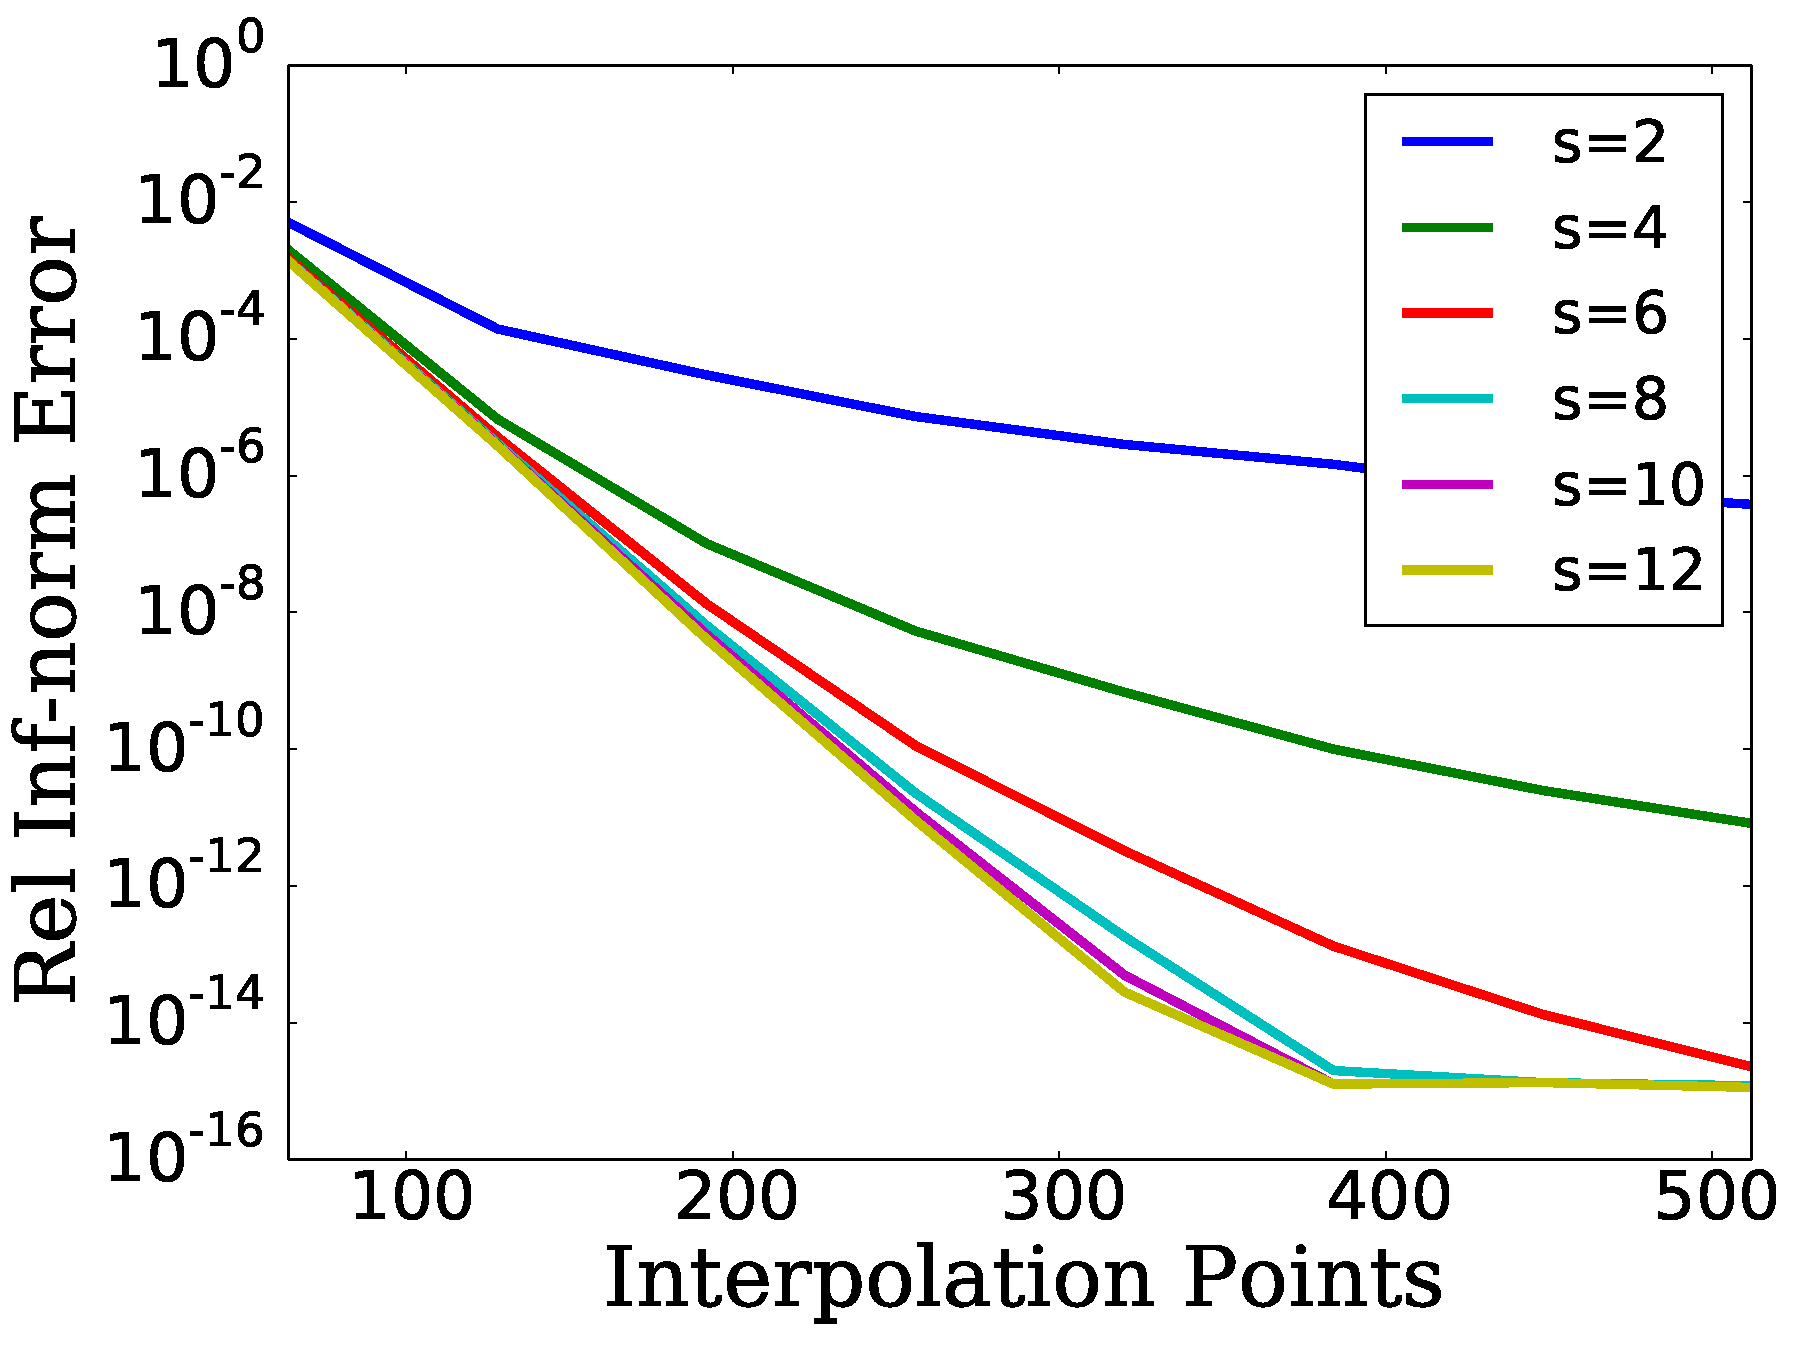
\includegraphics[width=\textwidth]{plots/msn_2n_fast_smooth_R_100_double.pdf}
    \caption{Double Precision}
    \end{subfigure}
    \begin{subfigure}{0.45\textwidth}
    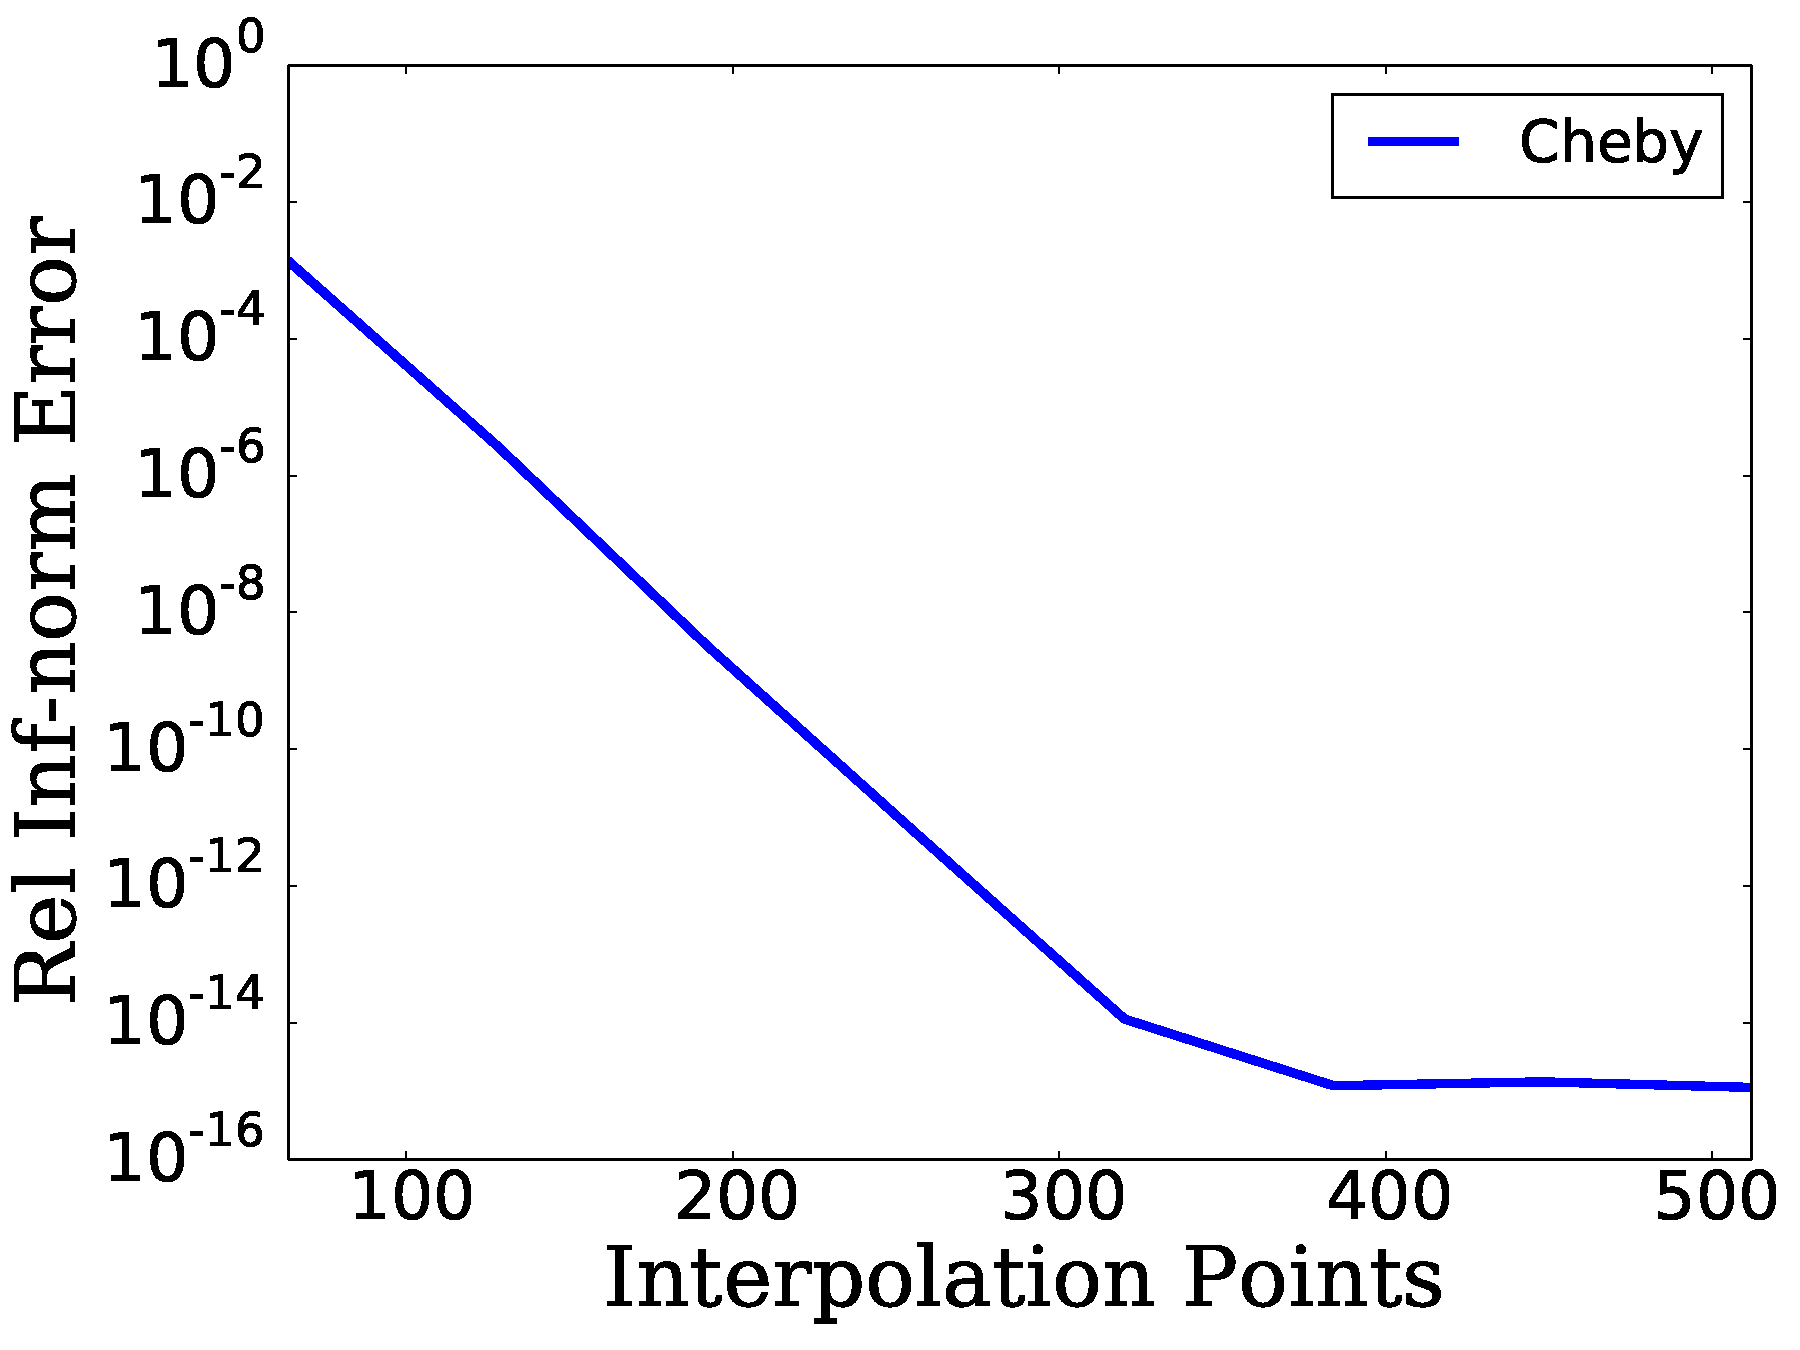
\includegraphics[width=\textwidth]{plots/cheby_interp_smooth_R_100_double.pdf}
    \caption{Double Precision}
    \end{subfigure}
\caption[Smooth Interpolation Comparison: 2D Runge Function $R=100$]{
MSN interpolation and Chebyshev inteprolation results
of the 2D Runge function $f_{100}$ for various $s$ values.
Here, $n$ interpolation points refers to interpolation on the $n\times n$
tensor grid of Chebyshev points.
}
\label{fig:smooth_comparison_2d_runge_100}
\end{figure}








\section{Gibbs Phenomenon and Smooth Cutoff Filters}

We now turn our attention from interpolating smooth functions
to interpolating rough functions.

The Gibbs phenomenon~\cite[Chapter 2]{zygmund} is a well-known problem
when one attempts to approximate a discontinuous function by a finite sum of
continuous functions, frequently chosen to be a Fourier series;
this is also true for Chebyshev expansions.
Recent work has been focused on determining filters
which smoothly cutoff the Fourier series; one review article
is~\cite{gottlieb1997gibbs}.
The filters $\sigma$ in the review article take the form
%
\begin{equation}
    f_{N}^{\sigma}(x) =
        \sum_{k=-\infty}^{\infty}\hat{f}_{k}\sigma\parens{\frac{k}{N}}e^{ikx},
\end{equation}
%
where $\sigma$ smoothly cuts off the higher order frequencies;
a more precise definition is given below.
This has a similar form of the smooth cutoff approximations
for the MSN method found in~\cite{msnInterp,msnBirkhoff}
as well as our proofs of Fast MSN convergence in
Chapter~\ref{chap:cvip_converge}.
In this way, MSN interpolation could be thought of as a smoothing
filter which acts in such a way so as to retain equality
at certain nodes (in this case, the Chebyshev interpolation nodes).
We will choose $s\in\braces{1,2,3,4,5,6}$ for our simulations,
although in practice $s$ can be any real number.

From~\cite{gottlieb1997gibbs}, we say a filter $\sigma$ is of order $p$ if
%
\begin{itemize}
\item $\sigma$ is an even function,
\item $\sigma(0) = 1$, $\sigma^{(\ell)}(0) = 0$ for $1\le\ell\le p-1$,
\item $\sigma(\eta) = 0$ for $\abs{\eta}\ge1$, and
\item $\sigma\in C^{p-1}$ for $\eta\in\parens{-\infty,\infty}$.
\end{itemize}

\noindent
We reproduce some of the filters from~\cite{gottlieb1997gibbs}
which we will use to compare with our MSN results.
In all instances, we set $\sigma(\eta) = 0$ when $\eta>1$.

\begin{itemize}
\item Chebyshev interpolation:
%
\begin{equation}
    \sigma_{0}(\eta) = 1.
\end{equation}
%
This results in no filtering but is kept as a baseline comparison.
Clearly $\sigma_{0}$ is not continuous at $\eta=1$.

\item The Fej\'{e}r filter:
%
\begin{equation}
    \sigma_{1}(\eta) = 1 - \eta.
\end{equation}

\item The Lanczos filter:
%
\begin{equation}
    \sigma_{2}(\eta) = \frac{\sin(\pi\eta)}{\pi\eta}.
\end{equation}
%
This is the normalized sinc function.

\item The Raised Cosine Filter:
%
\begin{equation}
    \sigma_{3}(\eta) = \frac{1}{2}\parens{1 + \cos(\pi\eta)}.
\end{equation}

\item The Sharpened Raised Cosine Filter:
%
\begin{equation}
    \sigma_{4}(\eta) = \sigma_{3}^{4}(\eta)\parens{
        35 - 84\sigma_{3}(\eta) + 70\sigma_{3}^{2}(\eta)
        - 20\sigma_{3}^{3}(\eta)}.
\end{equation}
%
This is an order 8 filter and will be denoted as ``Cos8'' in error plots.

\item The Exponential Filter of order $p$:
%
\begin{equation}
    \sigma_{5}(\eta) = \exp\parens{-\alpha\eta^{p}}.
\end{equation}
%
We will always take $p$ to be even and $\alpha = -\ln(\eps_{\text{mach}})$,
so that the largest frequency will be $O(\eps_{\text{mach}})$.
Naturally, $\sigma_{5}$ is not actually continuous at $\eta=1$.
\end{itemize}

\section{Functions for Rough Interpolation}

We will focus on interpolation where the function is not continuous
or whose derivatives are not continuous and compare the results
with standard Chebyshev interpolation and Chebyshev filters in 1D.
Because there are fewer theoretical results, we will focus on analyzing
some carefully chosen examples; in particular, we will
investigate interpolating
%
\begin{align}
    H(x) &= \begin{cases} 0 &x<0 \\ 1 &x\ge0 \end{cases} \nonumber\\
    H_{2}(x) &= H(x+\tfrac{1}{2}) + H(x) + H(x-\tfrac{1}{2}) \nonumber\\
    R(x) &= \begin{cases} \frac{1}{1+25x^{2}} &x<0 \\
                          \frac{2}{1+25x^{2}} &x\ge0 \end{cases} \nonumber\\
    G(x,\alpha) &= \abs{x}^{\alpha} \nonumber\\
    G_{2}(x,\alpha) &= G(x+\tfrac{1}{2},\alpha) + G(x,\alpha) +
        G(x-\tfrac{1}{2},\alpha).
\end{align}
%
Naturally, $H$ is the Heaviside function, $R$ has a jump discontinuity
between two Runge functions, and $G(\cdot,\alpha)$
has infinite derivatives at the origin when
$\alpha\in\parens{0,1}$.
All of these functions have difficulties at $x=0$, making them
challenging interpolation problems.
The error will be determined by computing the relative error at 1000 points
in $[-1,-0.1)\cup(0.1,1]$.
In the case of $H_{2}$ and $G_{2}$, the functions have multiple difficulties
and the relative error will be computed in the region
$[-1,-0.6)\cup(-0.4,-0.1)\cup(0.1,0.4)\cup(0.6,1]$.

\section{Results for Fast MSN Interpolation in 1D for Rough Functions}
\label{sec:rough_1D_sim}

\subsection{Interpolation Comparison}

The relative error results for the Heaviside function $H$ can be found in
Fig.~\ref{fig:rough_comparison_heaviside},
the results for the Runge jump function $R(x)$ can be found in
Fig.~\ref{fig:rough_comparison_runge_jump}, and
the results for $G(\cdot,0.5)$ can be found in
Fig.~\ref{fig:rough_comparison_sharp_func}.
In the case of having multiple difficulties, 
the results for $H_{2}$ can be found in
Fig.~\ref{fig:rough_comparison_heaviside_2}, while
the results for $G_{2}(\cdot,0.5)$ can be found in
Fig.~\ref{fig:rough_comparison_sharp_func_2}.
We note that the Sharpened Cosine Filter $\sigma_{4}$ is denoted
by ``Cos8'' in the legend.
We will keep the unfiltered Chebyshev interpolant in both filter plots
for reference.

In every instance, MSN interpolation with $s=4$ appears to have the
quickest error decrease while also reaching machine precision first.
The best Chebyshev filters appear to to be the Sharpened Cosine filter (Cos8)
as well as the higher order Exponential filters (order 6 and 8).
The error profiles are approximately the same in every instance,
regardless of whether the function is discontinuous ($H$ and $R$),
has infinite derivatives ($G$), or multiple jumps or infinite derivatives
($H_{2}$ and $G_{2}$).
The worst case for MSN interpolation is when $s=1$.
Even in this case, it has lower error than the Chebyshev,
Fej\'{e}r, Lanczos, Cosine, and Exp 2 filters in most instances.
To make the comparison clear, in Fig.~\ref{fig:msn_filter_comp_heaviside_2}
where we plot the minimum error for both MSN interpolation
and Chebyshev filters for the $H_{2}$ function.
As we can see, the minimal MSN error usually approximately the same or better
than the best filters.
To see how different $s$ values in MSN affect interpolation
results, we include plots for various $s$ values and interpolation
points when approximating $H_{2}$ in Fig.~\ref{fig:msn_n_s_heaviside_2}.

In these examples so far we only used polynomials of degree $2n$
for $n$ interpolation points; we have included results for
degree $2n$, $4n$, $6n$, and $8n$ interpolation
in Fig.~\ref{fig:msn_comp_degree} when attempting to interpolate $H_{2}$.
As we can see, there is little difference between them.
The difference in using larger interpolation degree only becomes
apparent when using small $s$ values, such as when $s\in\parens{0,1}$.
By looking at the explicit form of the coefficients, we see
that they do not play a large part; furthermore, by construction,
once the IDCT gives somewhat accurate approximates of the true
Chebyshev coefficients, larger $s$ values closely match the
first $n$ coefficients while also matching the interpolation constraints.
Thus, degree $2n$ MSN interpolation appears sufficient in these tests.

% Print results for comparing MSN with Heaviside jump function

\begin{figure}[p]
    \centering
    \begin{subfigure}{0.45\textwidth}
    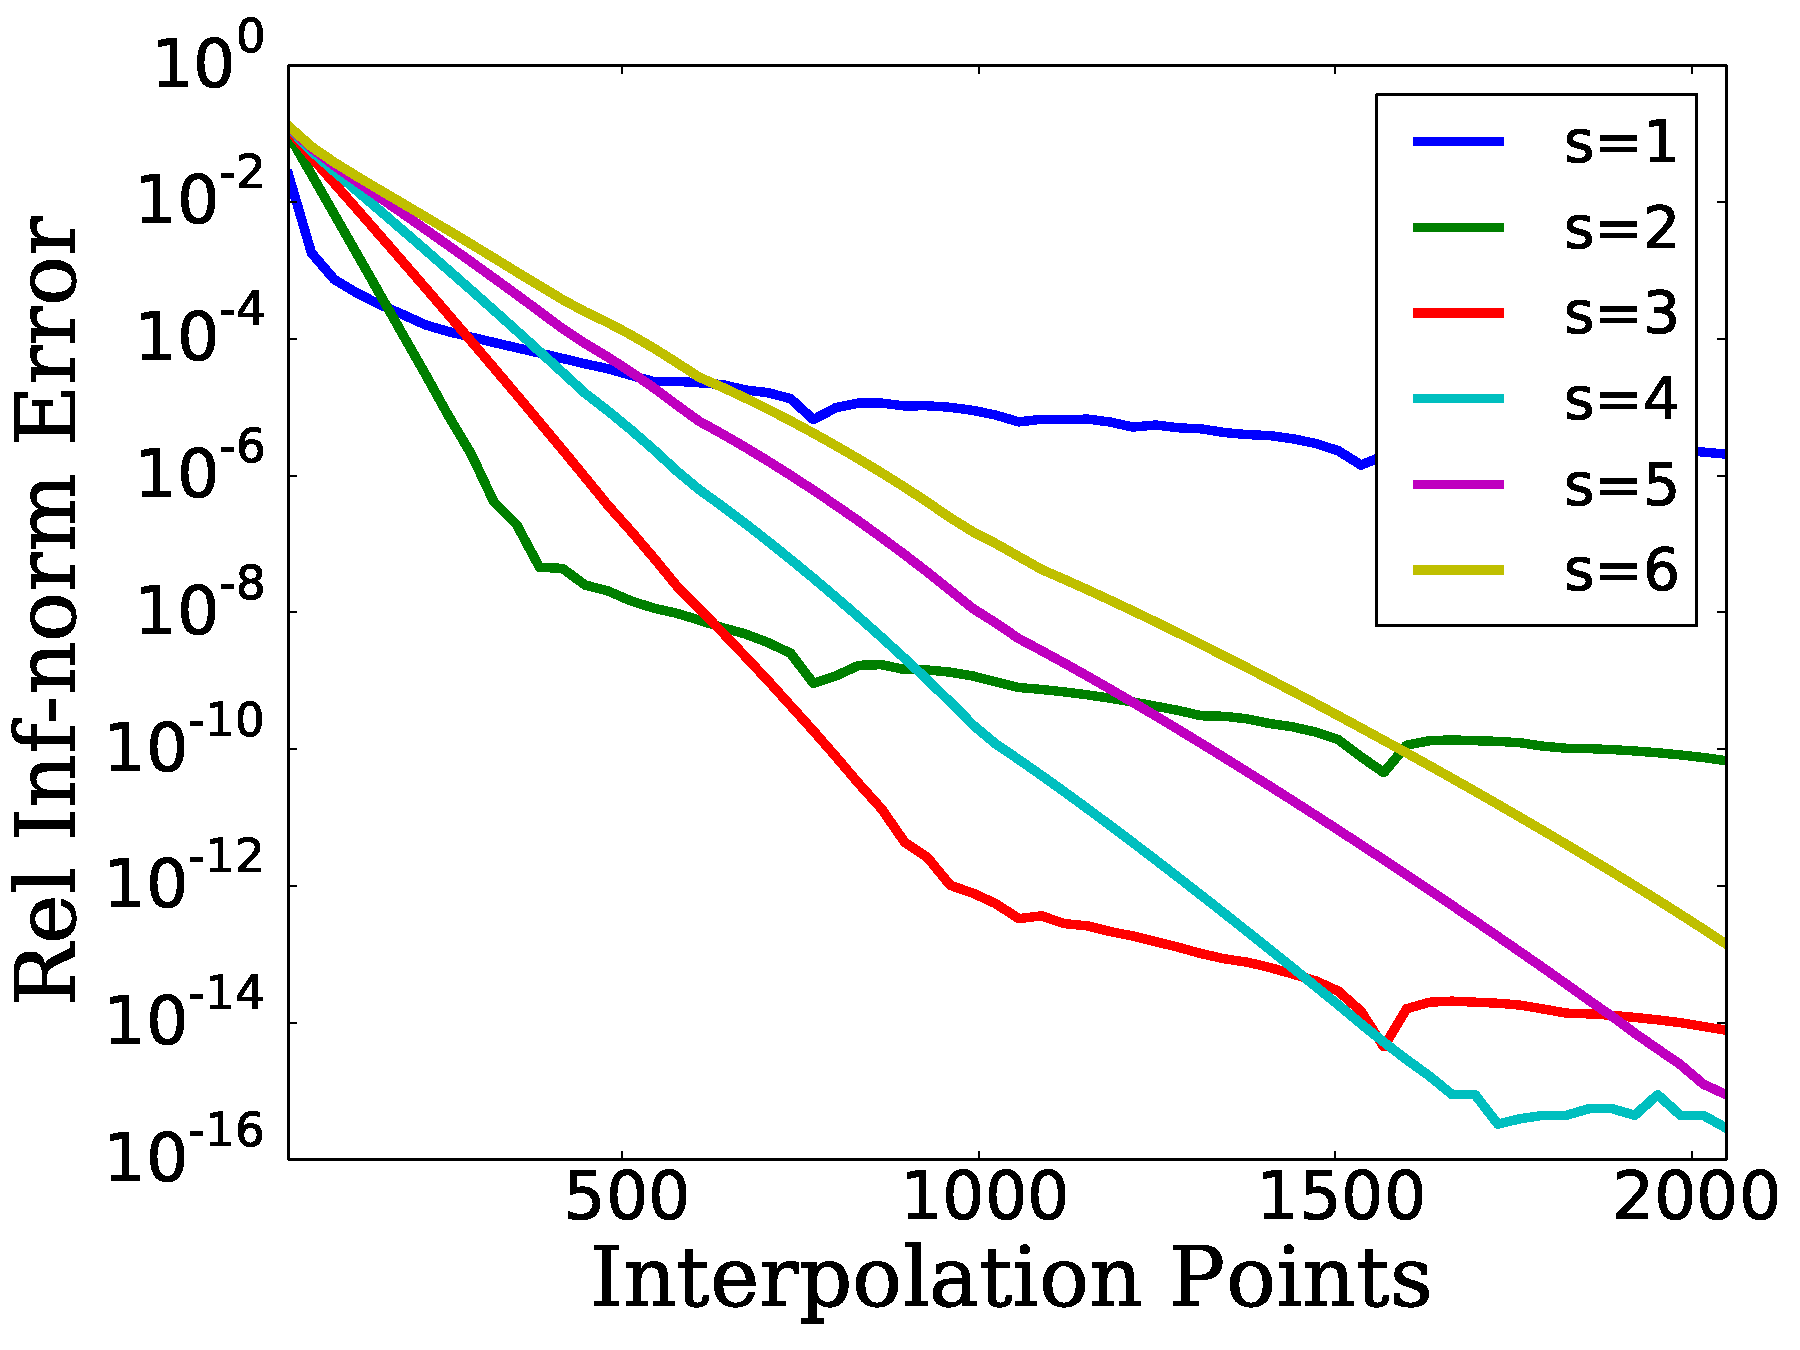
\includegraphics[width=\textwidth]{plots/msn_interp_fast_2n_rough_heaviside.pdf}
    \caption{MSN Interpolation}
    \end{subfigure}

    \begin{subfigure}{0.45\textwidth}
    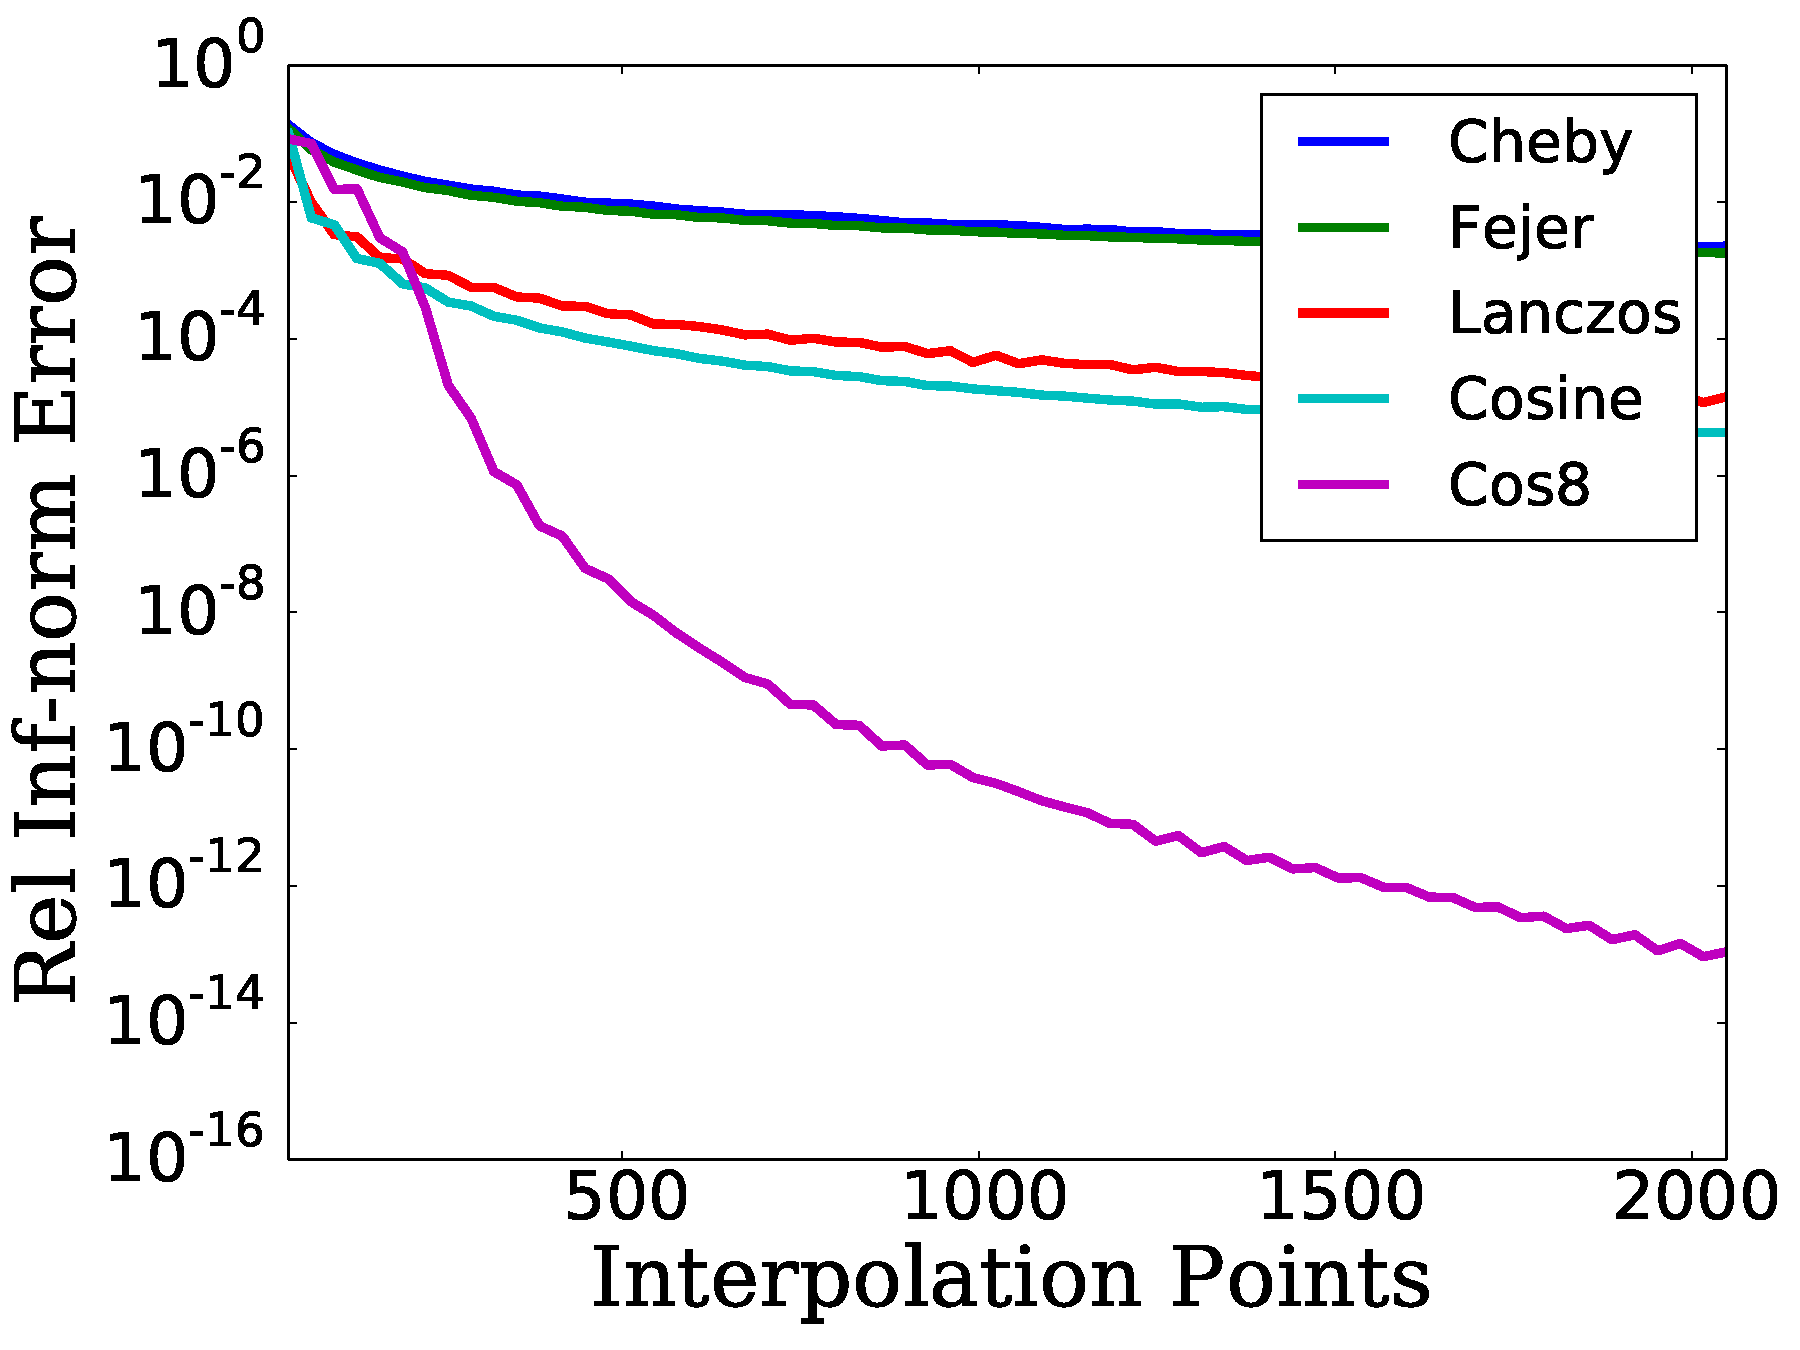
\includegraphics[width=\textwidth]{plots/cheby_interp_filter_rough_heaviside.pdf}
    \caption{Filters, Plot 1}
    \end{subfigure}
    \begin{subfigure}{0.45\textwidth}
    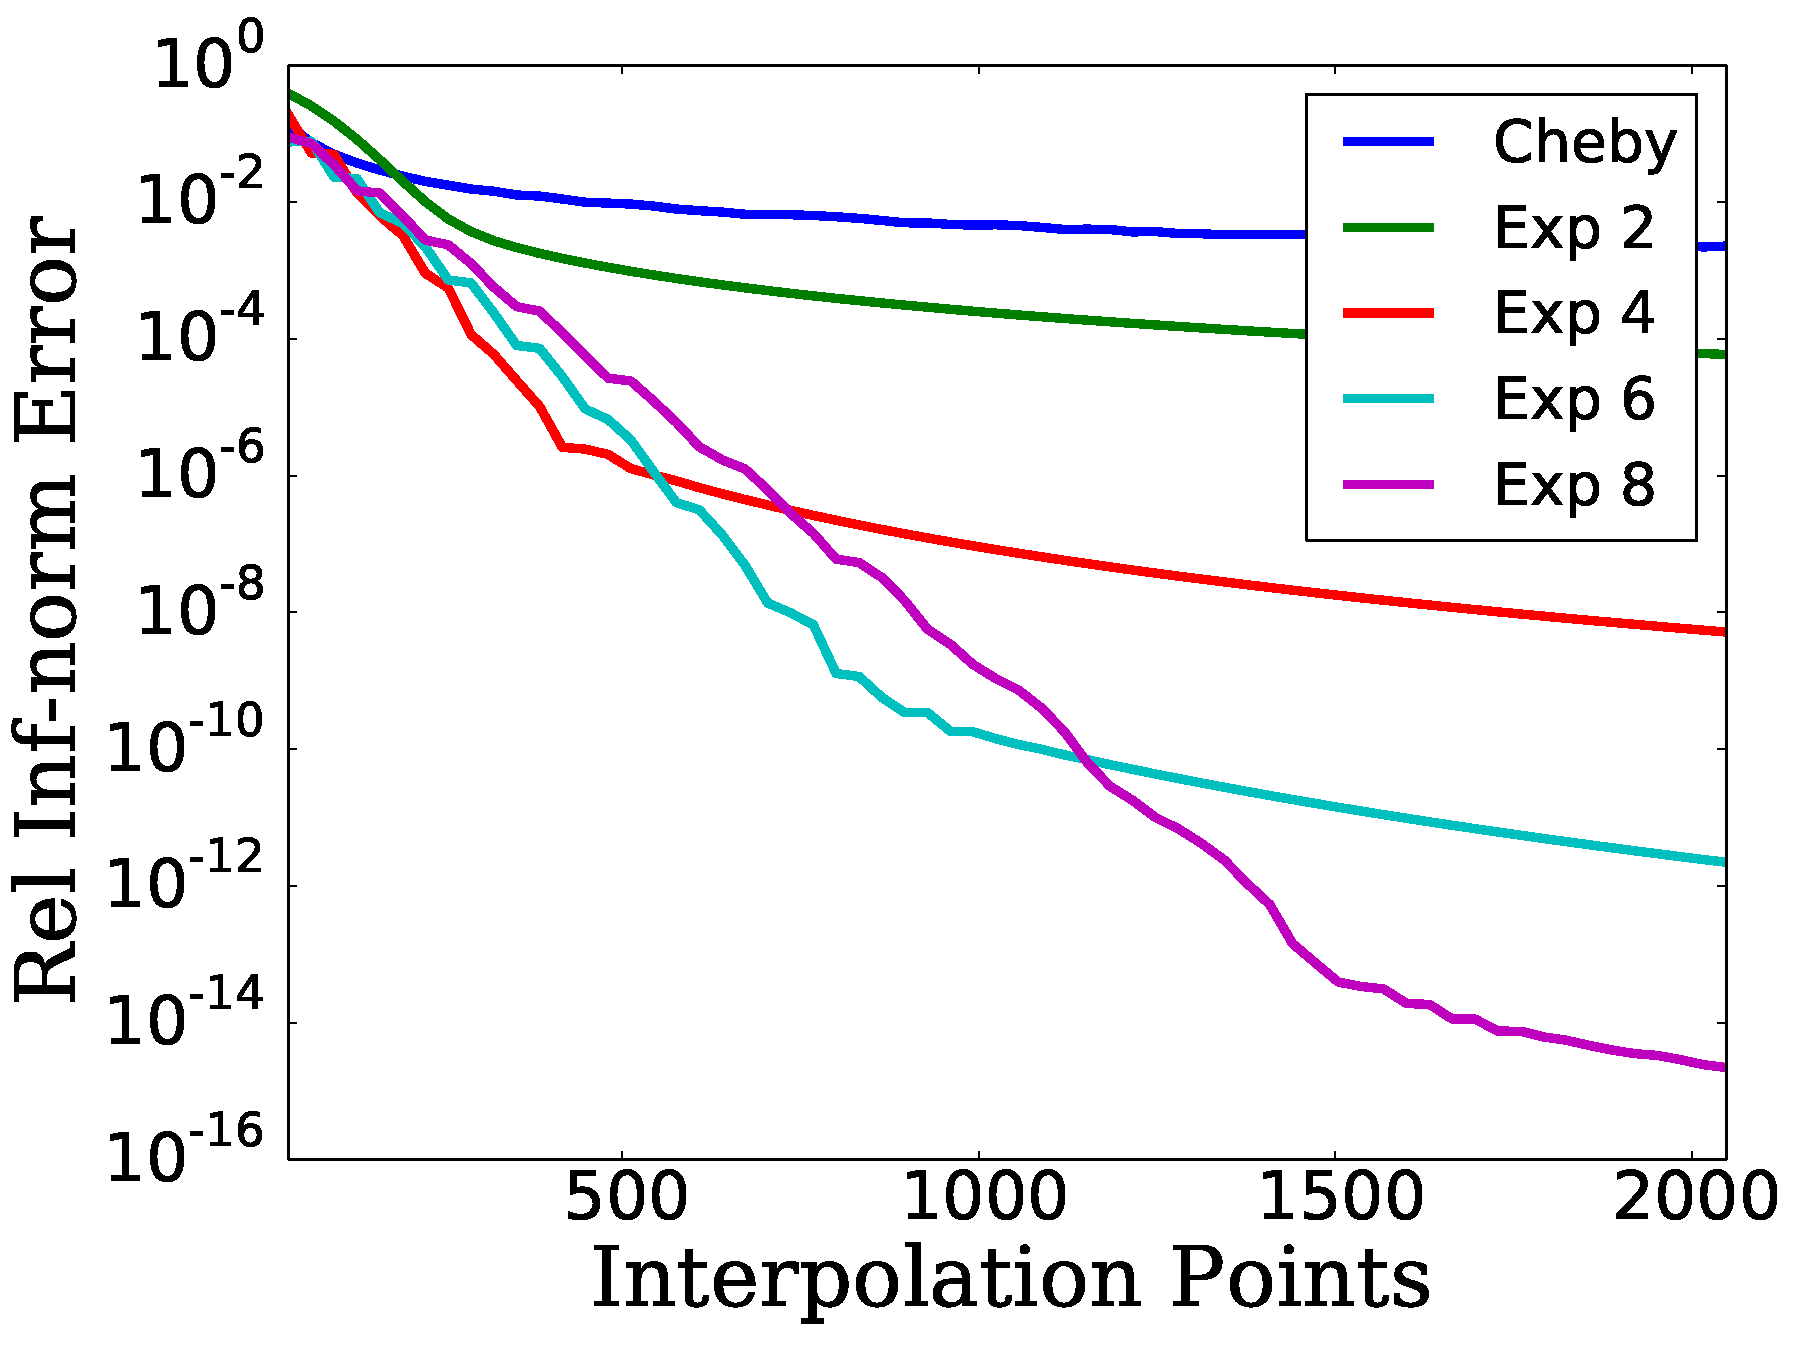
\includegraphics[width=\textwidth]{plots/cheby_interp_filter_2_rough_heaviside.pdf}
    \caption{Filters, Plot 2}
    \end{subfigure}
\caption[Rough Interpolation Comparison: Heaviside Jump Function]{
MSN interpolation and Chebyshev filtering results of the Heaviside jump
function $H$ for various $s$ values and filters.
We include standard Chebyshev interpolant in both filter examples for reference.
}
\label{fig:rough_comparison_heaviside}
\end{figure}




% Print results for comparing MSN with Heaviside jump function

\begin{figure}[p]
    \centering
    \begin{subfigure}{0.45\textwidth}
    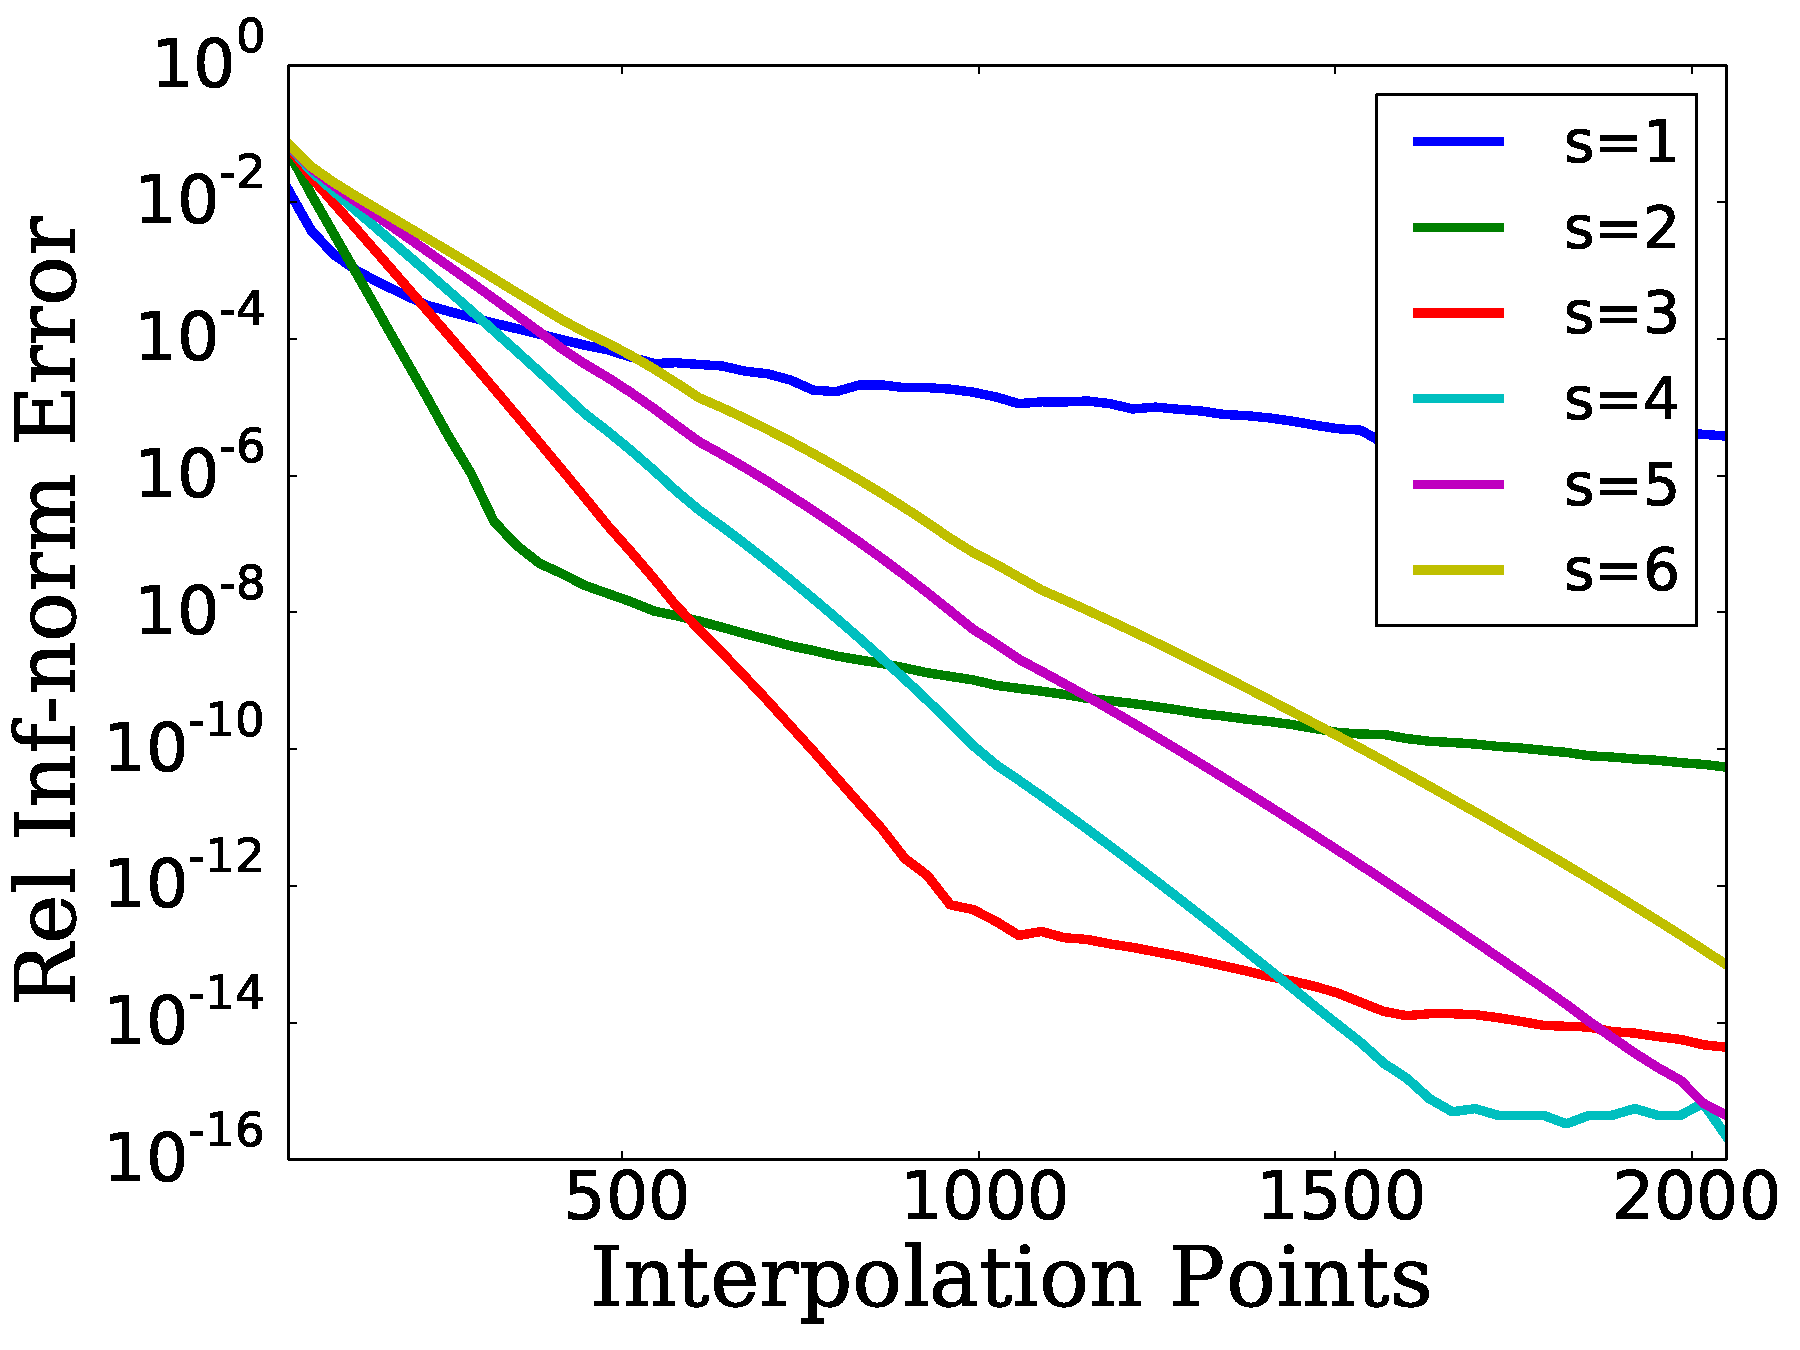
\includegraphics[width=\textwidth]{plots/msn_interp_fast_2n_rough_runge_jump.pdf}
    \caption{MSN Interpolation}
    \end{subfigure}

    \begin{subfigure}{0.45\textwidth}
    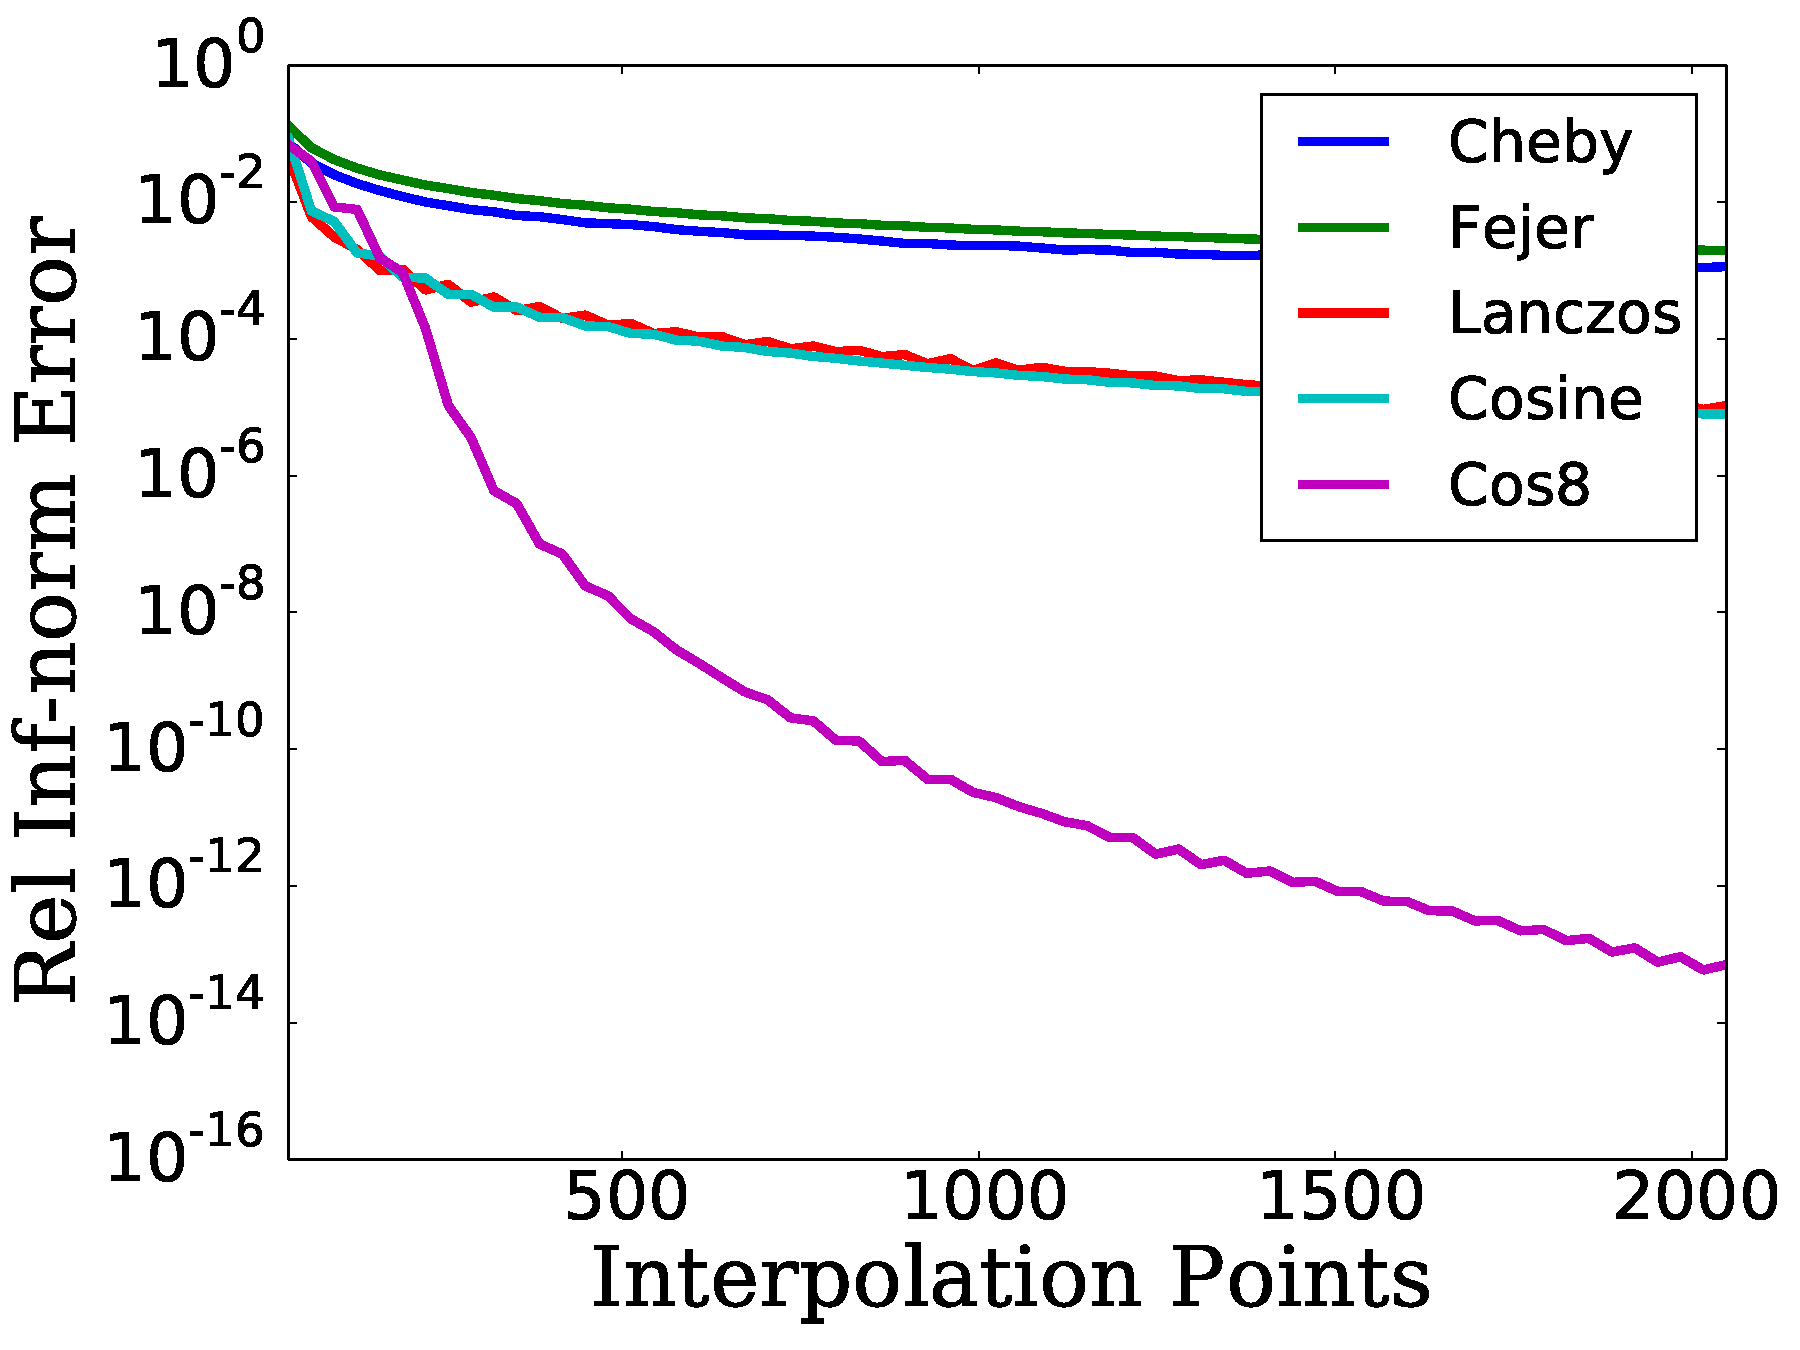
\includegraphics[width=\textwidth]{plots/cheby_interp_filter_rough_runge_jump.pdf}
    \caption{Filters, Plot 1}
    \end{subfigure}
    \begin{subfigure}{0.45\textwidth}
    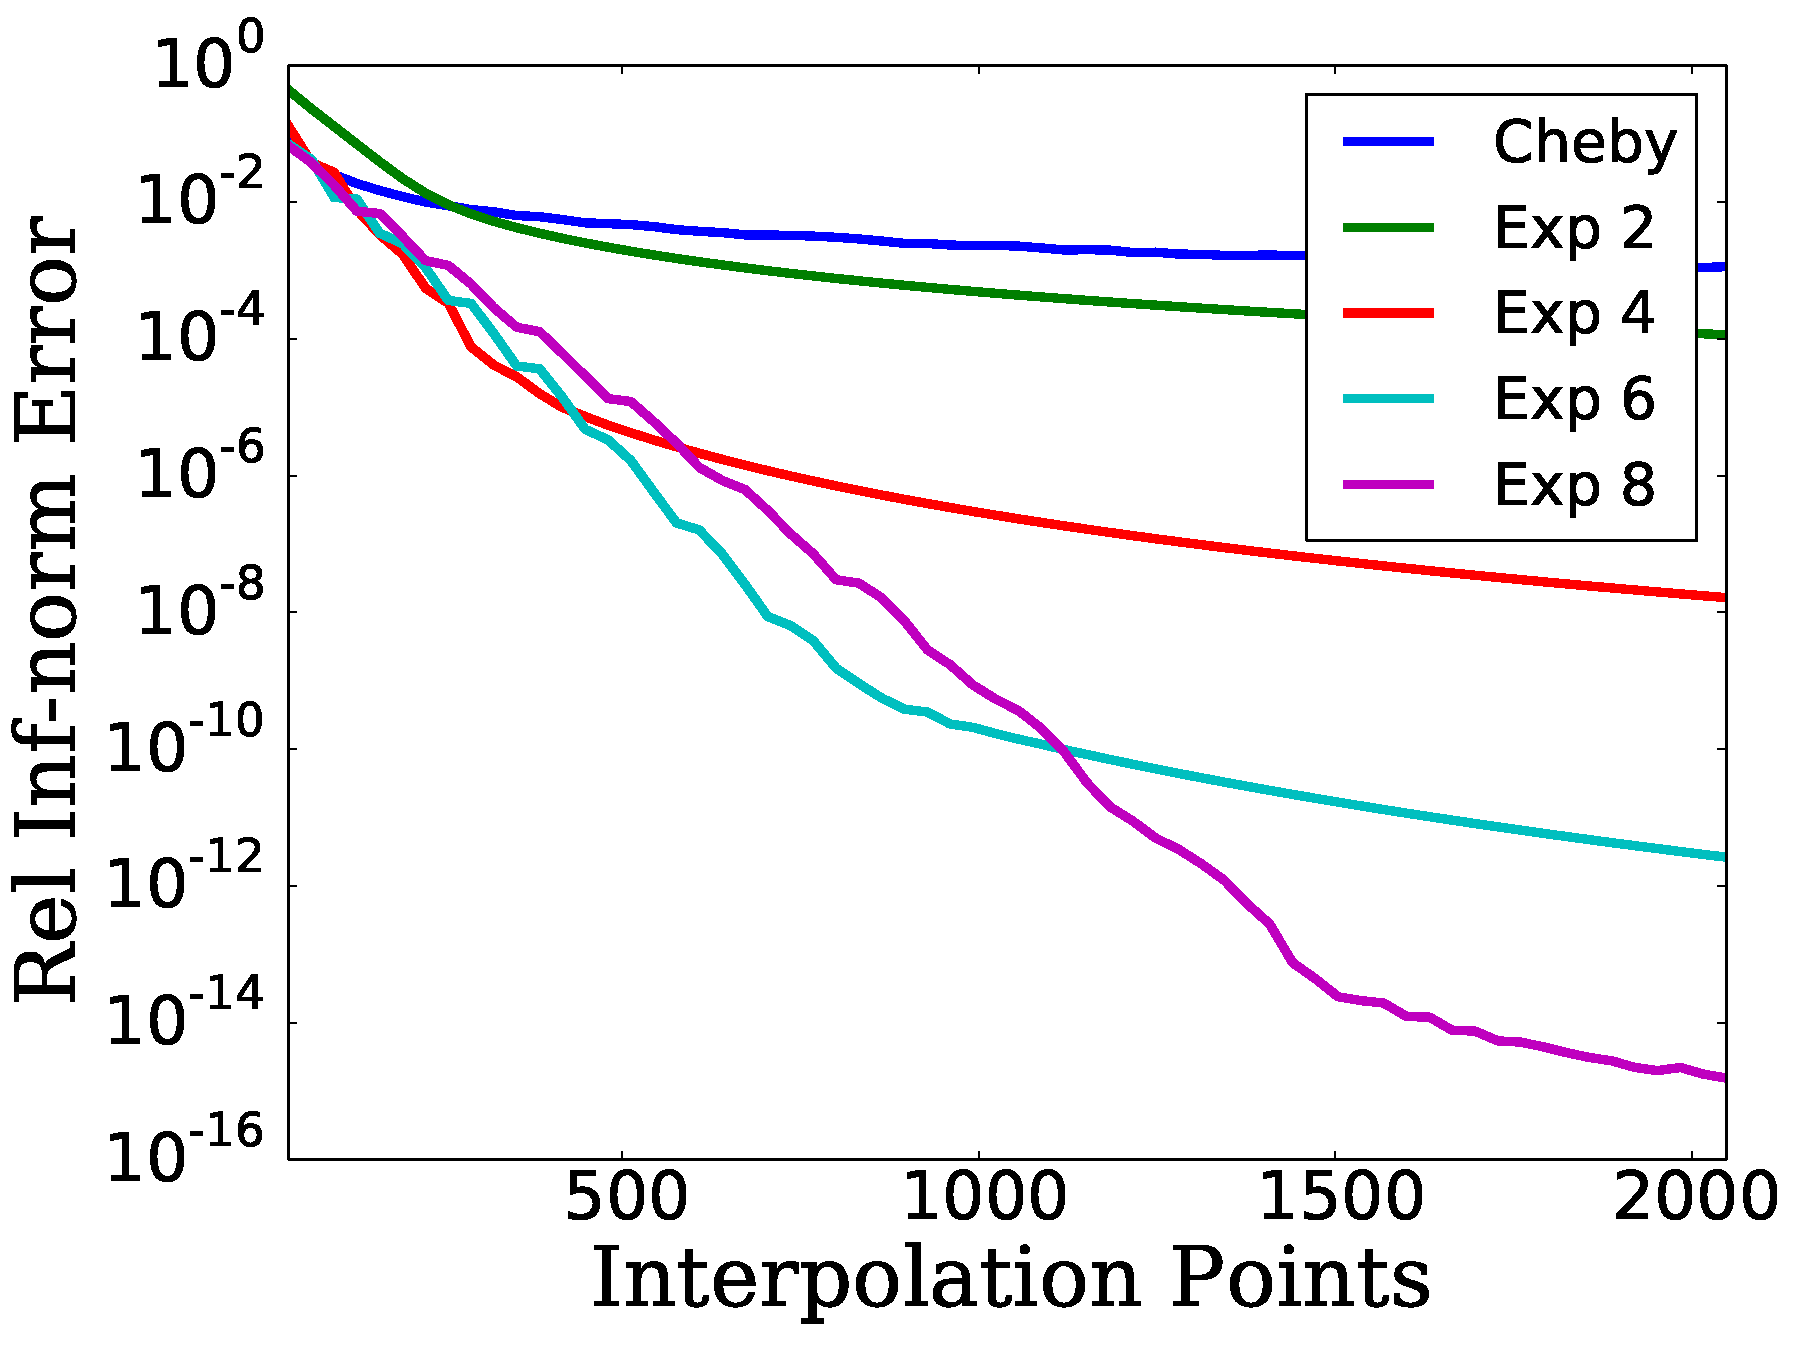
\includegraphics[width=\textwidth]{plots/cheby_interp_filter_2_rough_runge_jump.pdf}
    \caption{Filters, Plot 2}
    \end{subfigure}
\caption[Rough Interpolation Comparison: Runge Jump Function]{
MSN interpolation and Chebyshev filtering results of the Runge jump
function $R$ for various $s$ values and filters.
We include standard Chebyshev interpolant in both filter examples for reference.
}
\label{fig:rough_comparison_runge_jump}
\end{figure}




% Print results for comparing MSN with Heaviside jump function

\begin{figure}[p]
    \centering
    \begin{subfigure}{0.45\textwidth}
    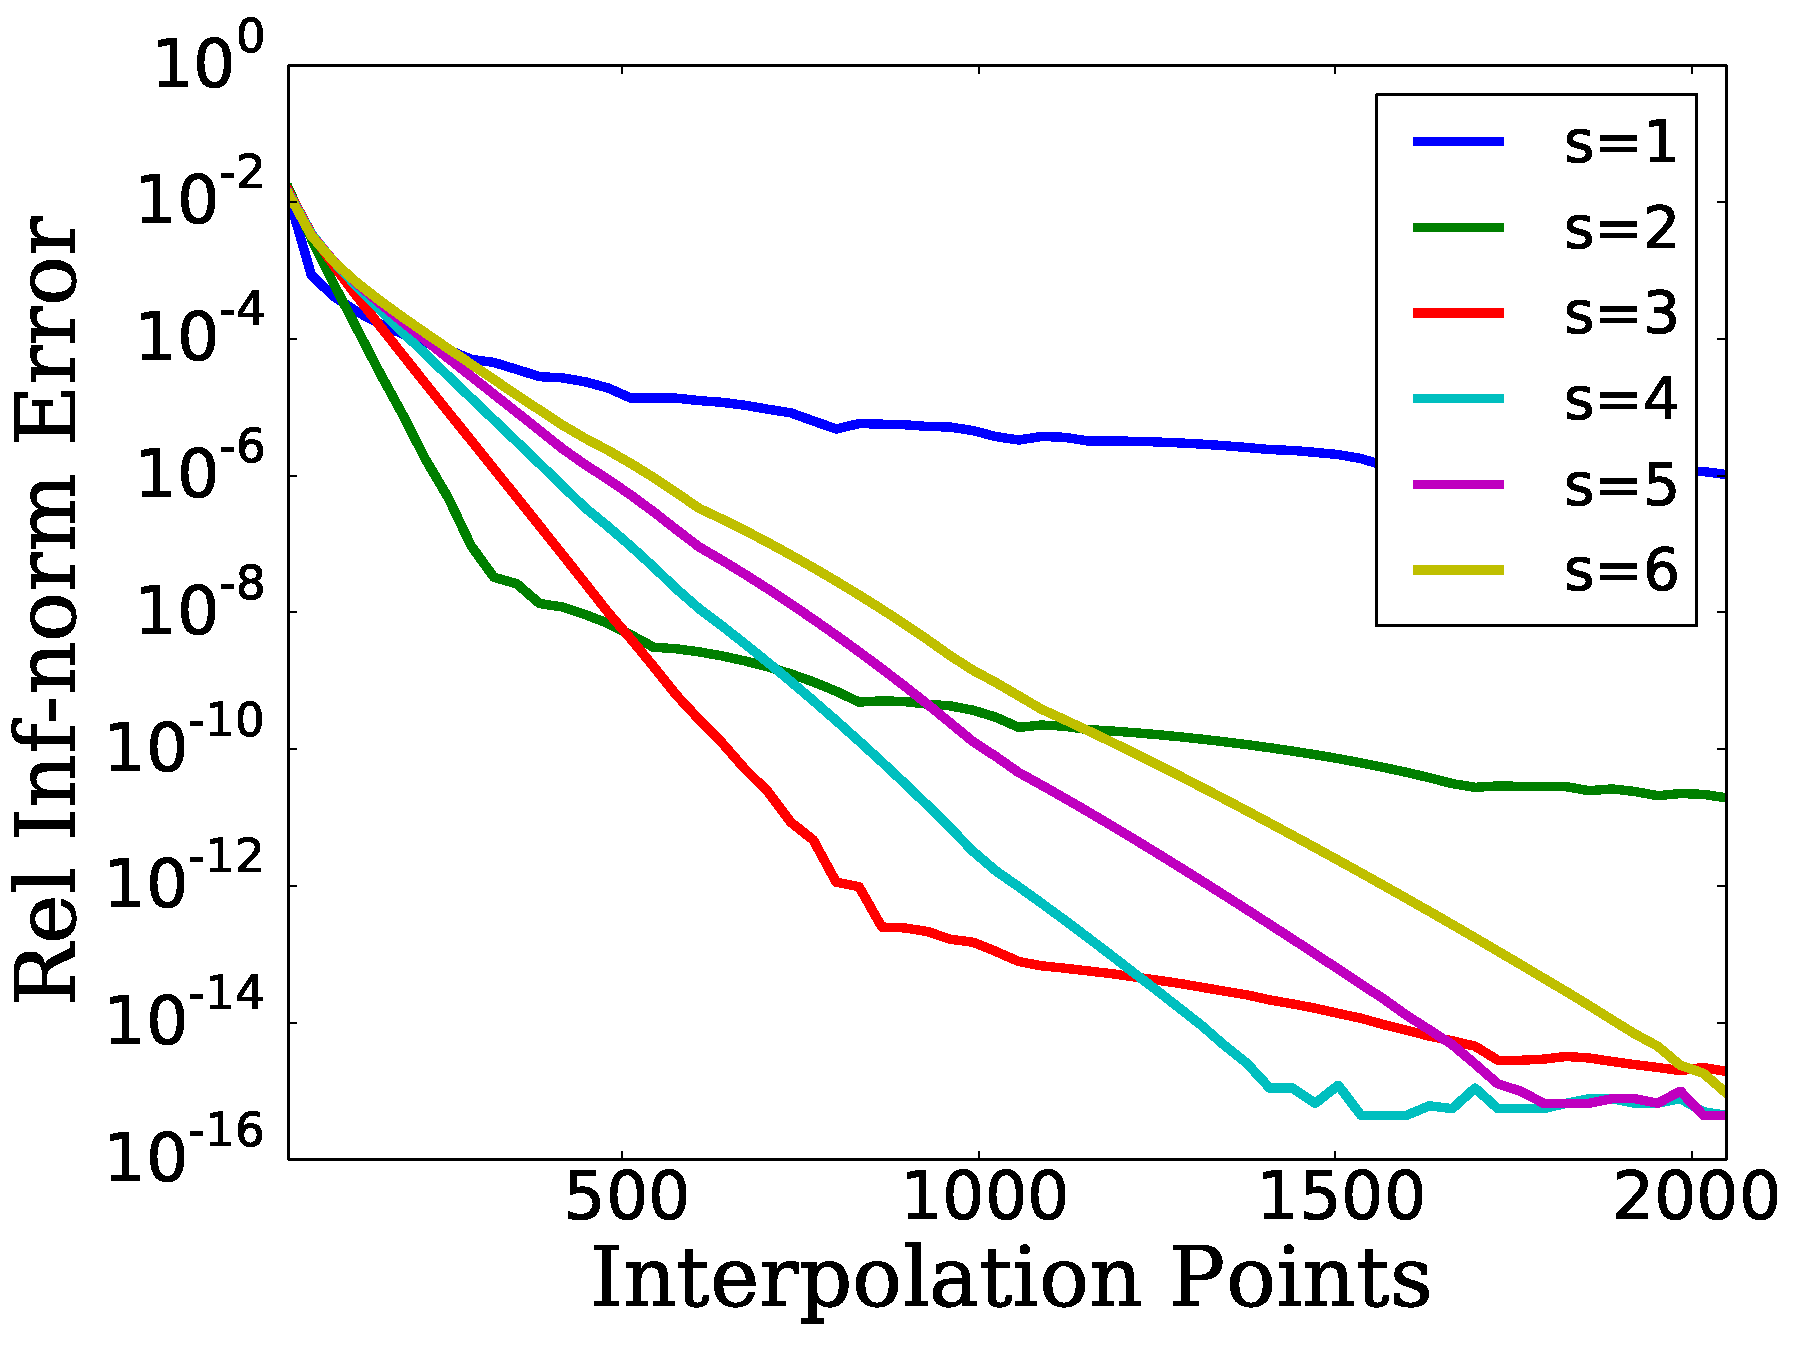
\includegraphics[width=\textwidth]{plots/msn_interp_fast_2n_rough_sharp_func.pdf}
    \caption{MSN Interpolation}
    \end{subfigure}

    \begin{subfigure}{0.45\textwidth}
    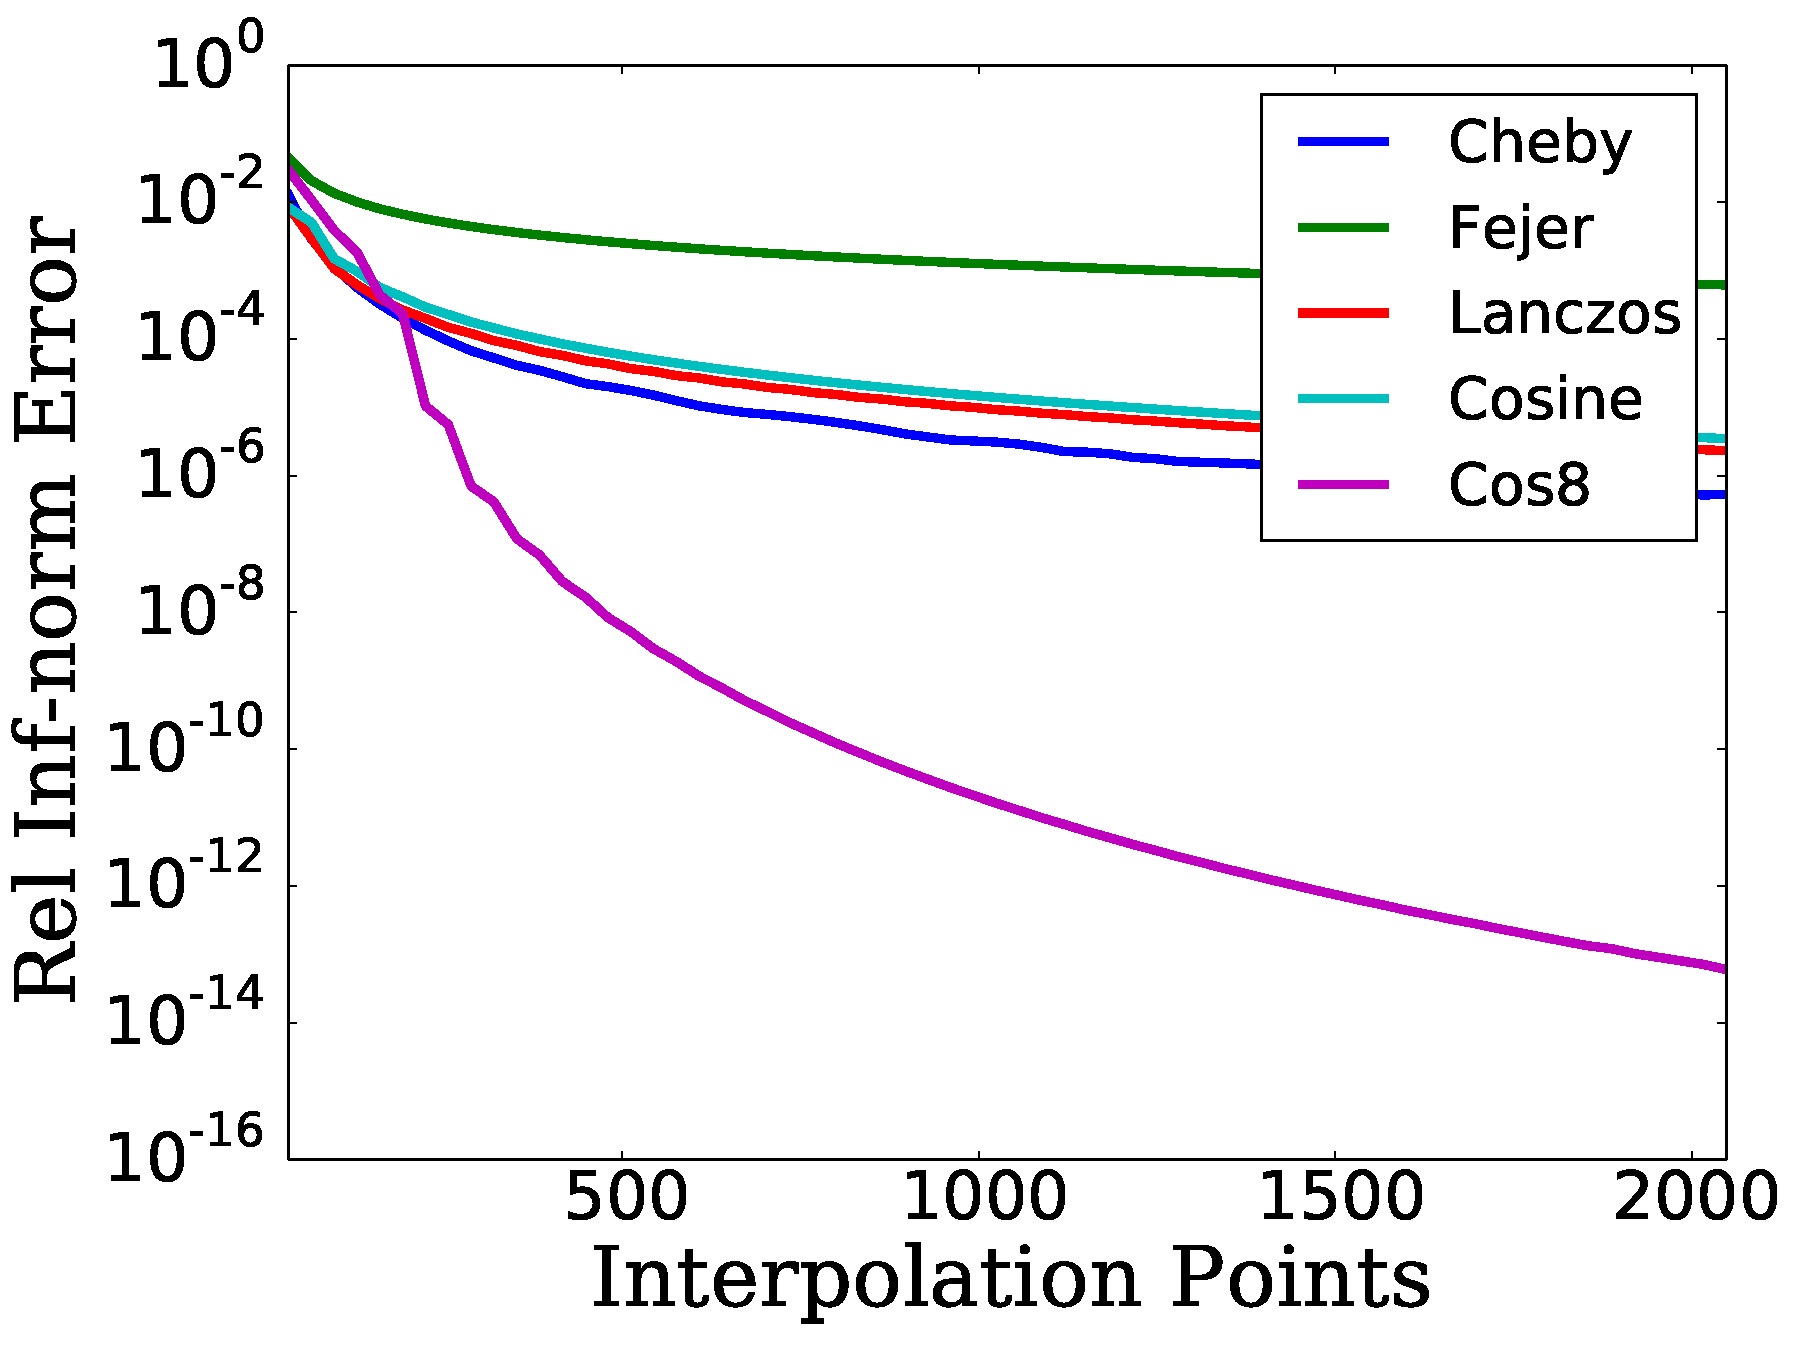
\includegraphics[width=\textwidth]{plots/cheby_interp_filter_rough_sharp_func.pdf}
    \caption{Filters, Plot 1}
    \end{subfigure}
    \begin{subfigure}{0.45\textwidth}
    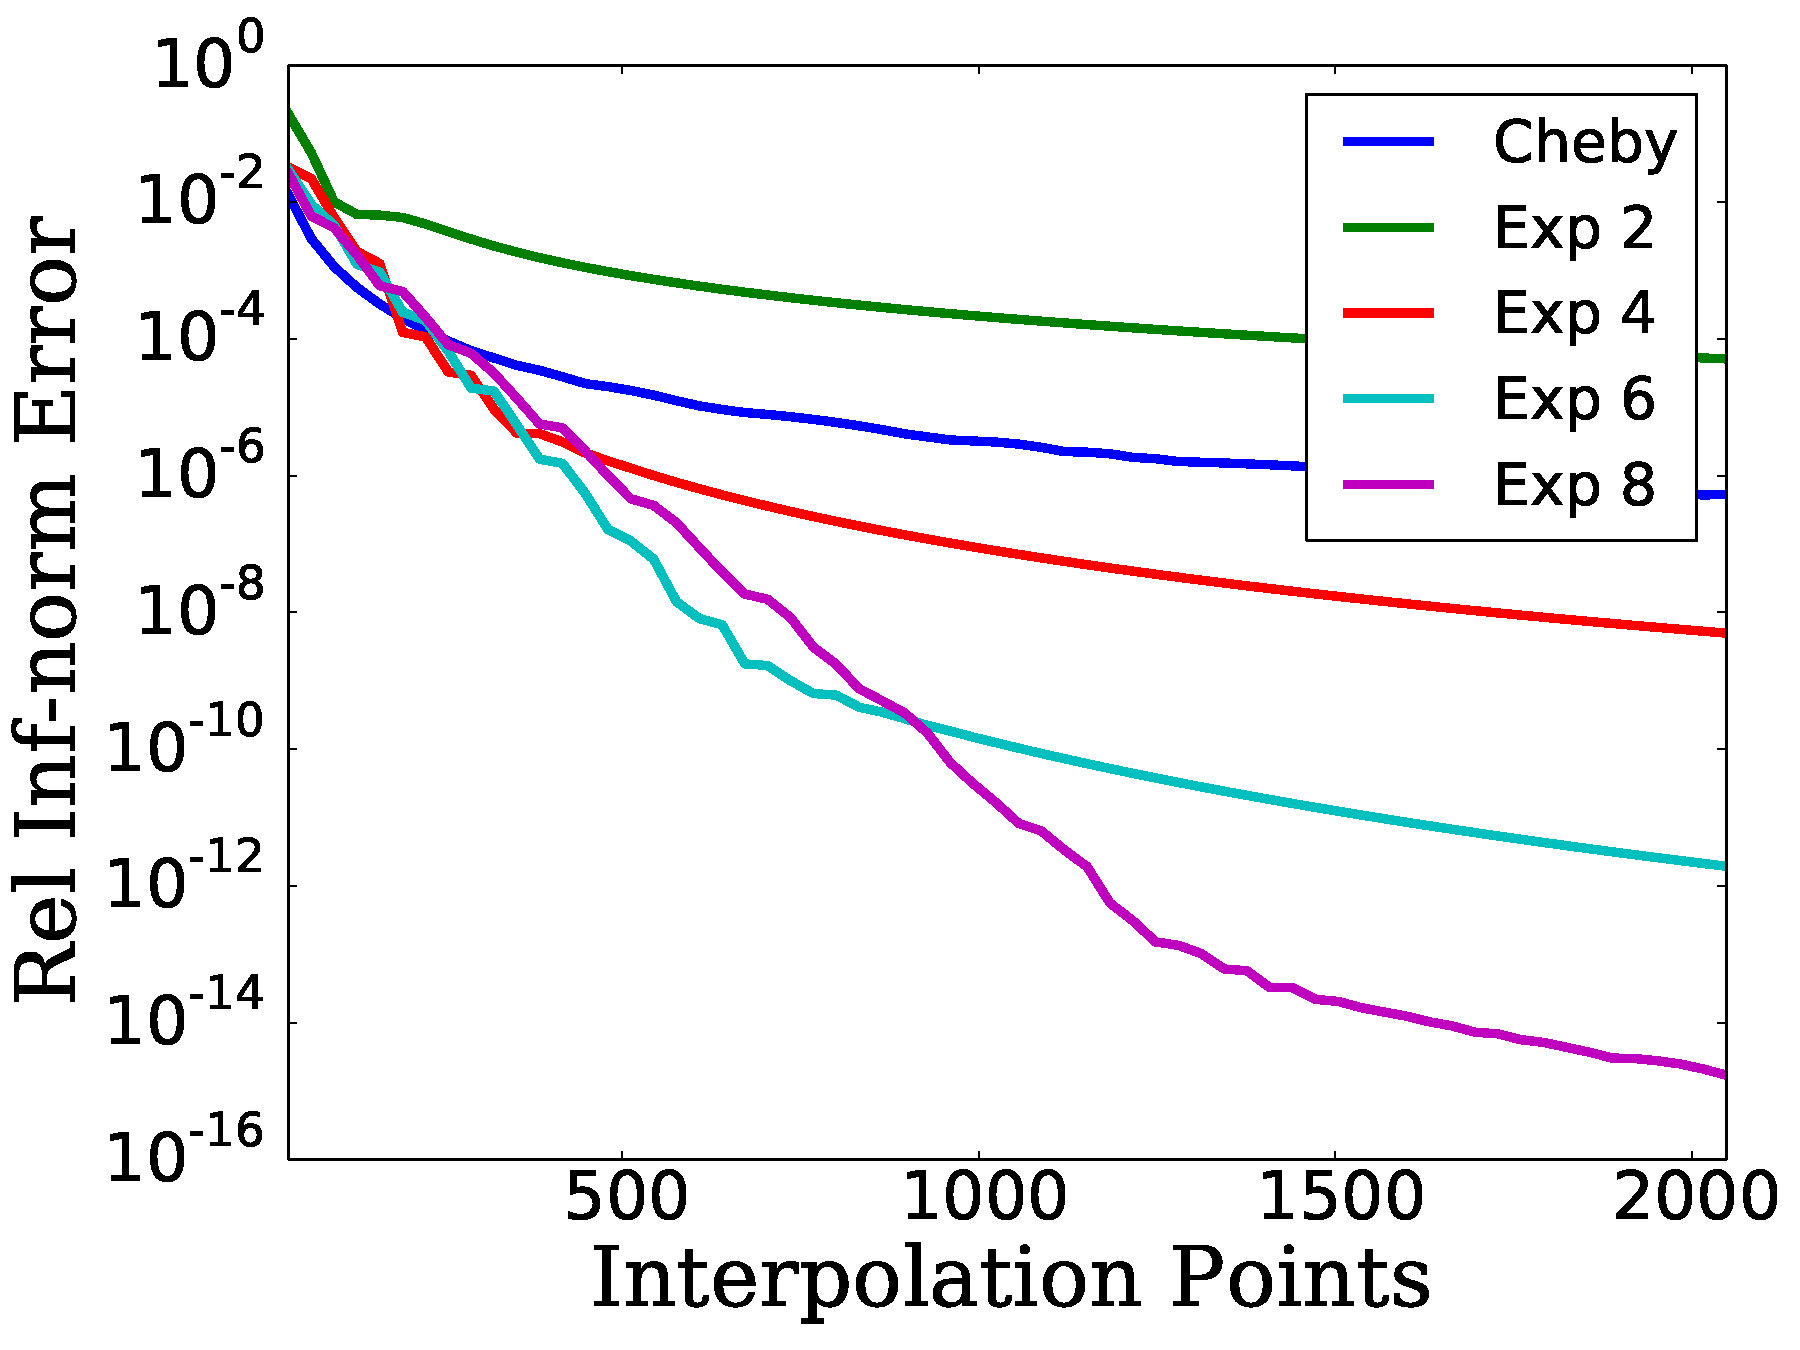
\includegraphics[width=\textwidth]{plots/cheby_interp_filter_2_rough_sharp_func.pdf}
    \caption{Filters, Plot 2}
    \end{subfigure}
\caption[Rough Interpolation Comparison: Sharp Function]{
MSN interpolation and Chebyshev filtering results of the Sharp Function
$G(\cdot,0.5)$ for various $s$ values and filters.
We include standard Chebyshev interpolant in both filter examples for reference.
}
\label{fig:rough_comparison_sharp_func}
\end{figure}




% Print results for comparing MSN with Heaviside jump function

\begin{figure}[p]
    \centering
    \begin{subfigure}{0.45\textwidth}
    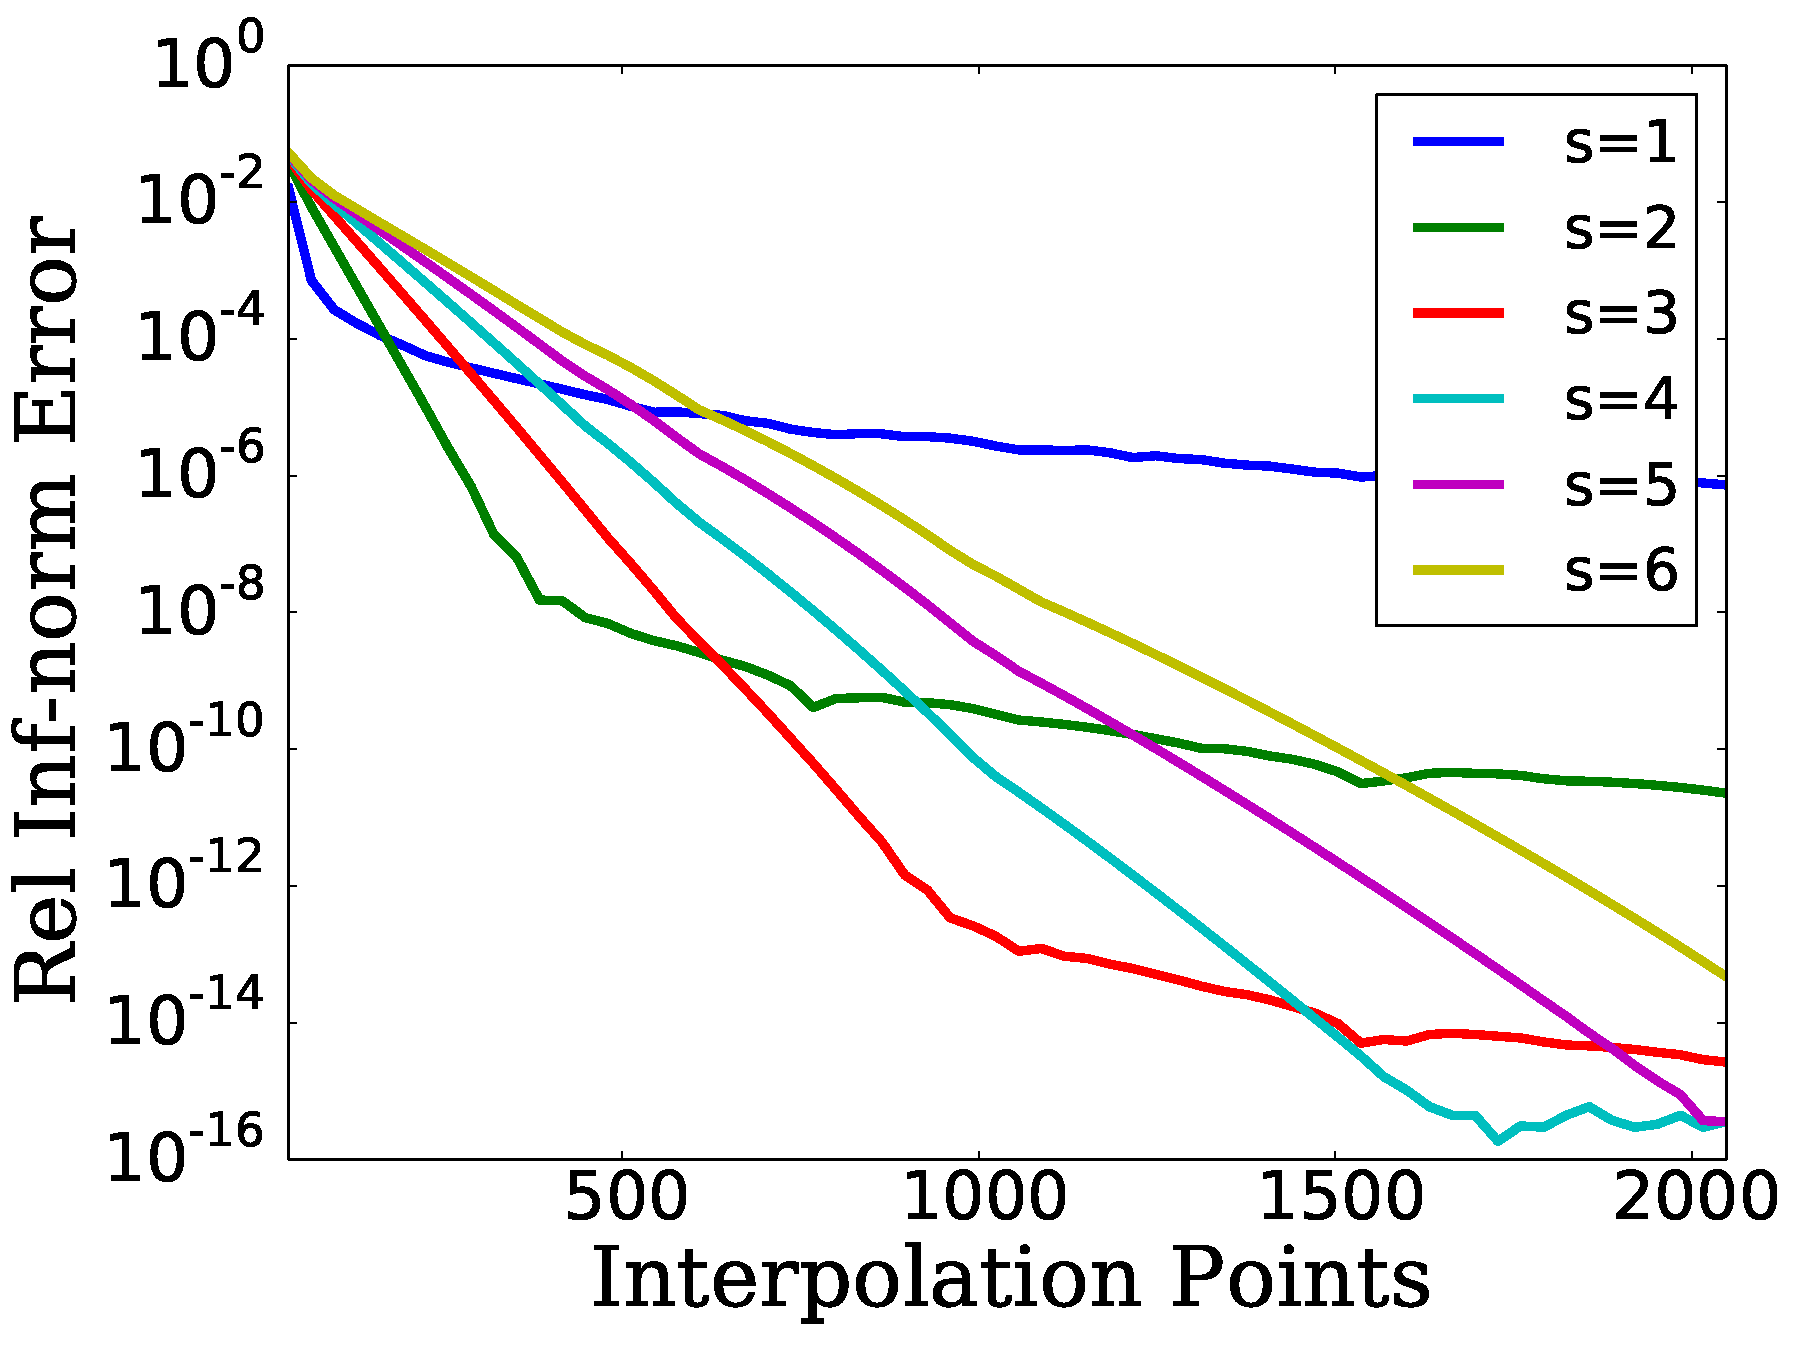
\includegraphics[width=\textwidth]{plots/msn_interp_fast_2n_rough_heaviside_2.pdf}
    \caption{MSN Interpolation}
    \end{subfigure}

    \begin{subfigure}{0.45\textwidth}
    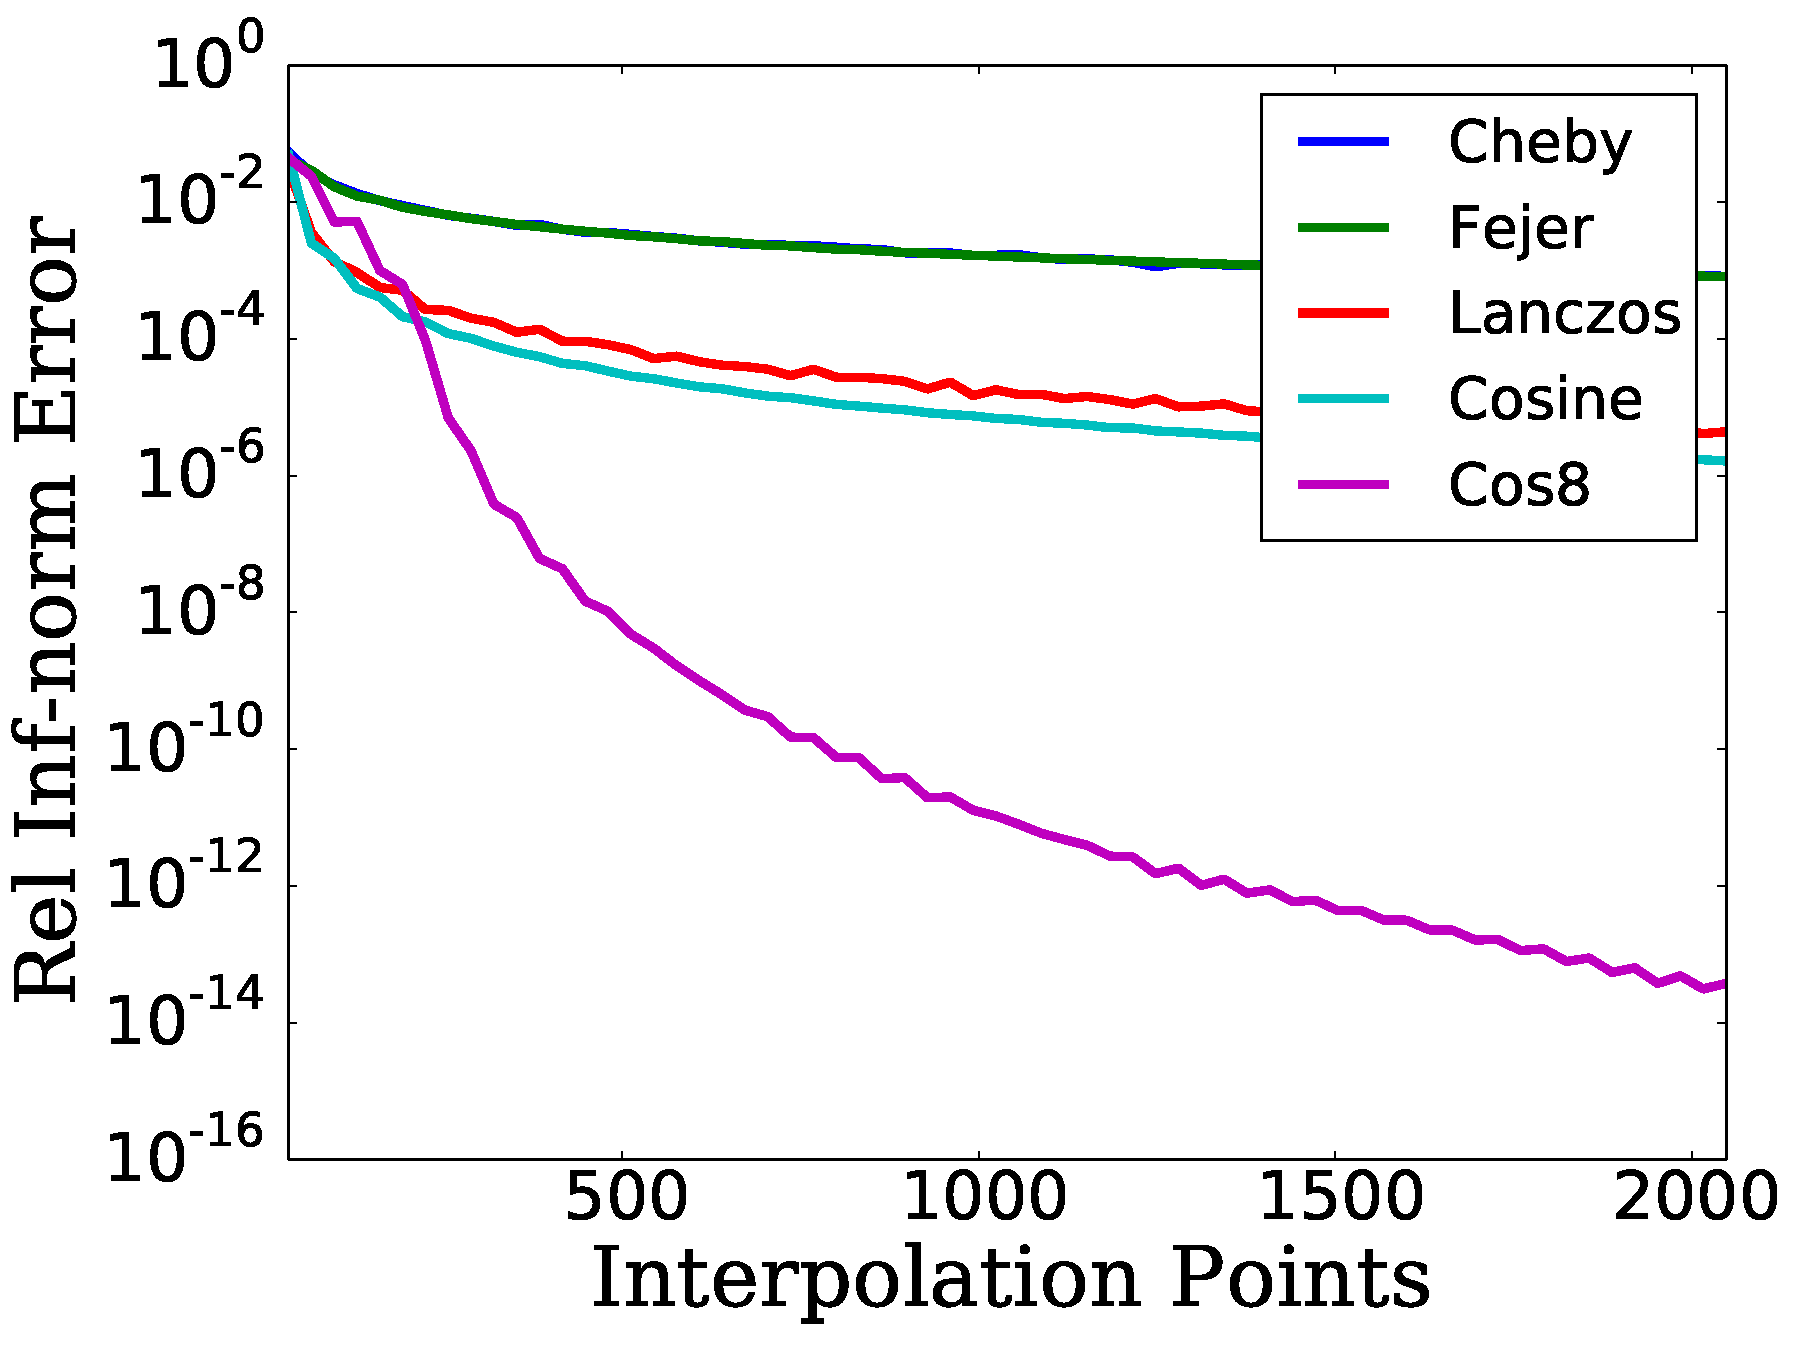
\includegraphics[width=\textwidth]{plots/cheby_interp_filter_rough_heaviside_2.pdf}
    \caption{Filters, Plot 1}
    \end{subfigure}
    \begin{subfigure}{0.45\textwidth}
    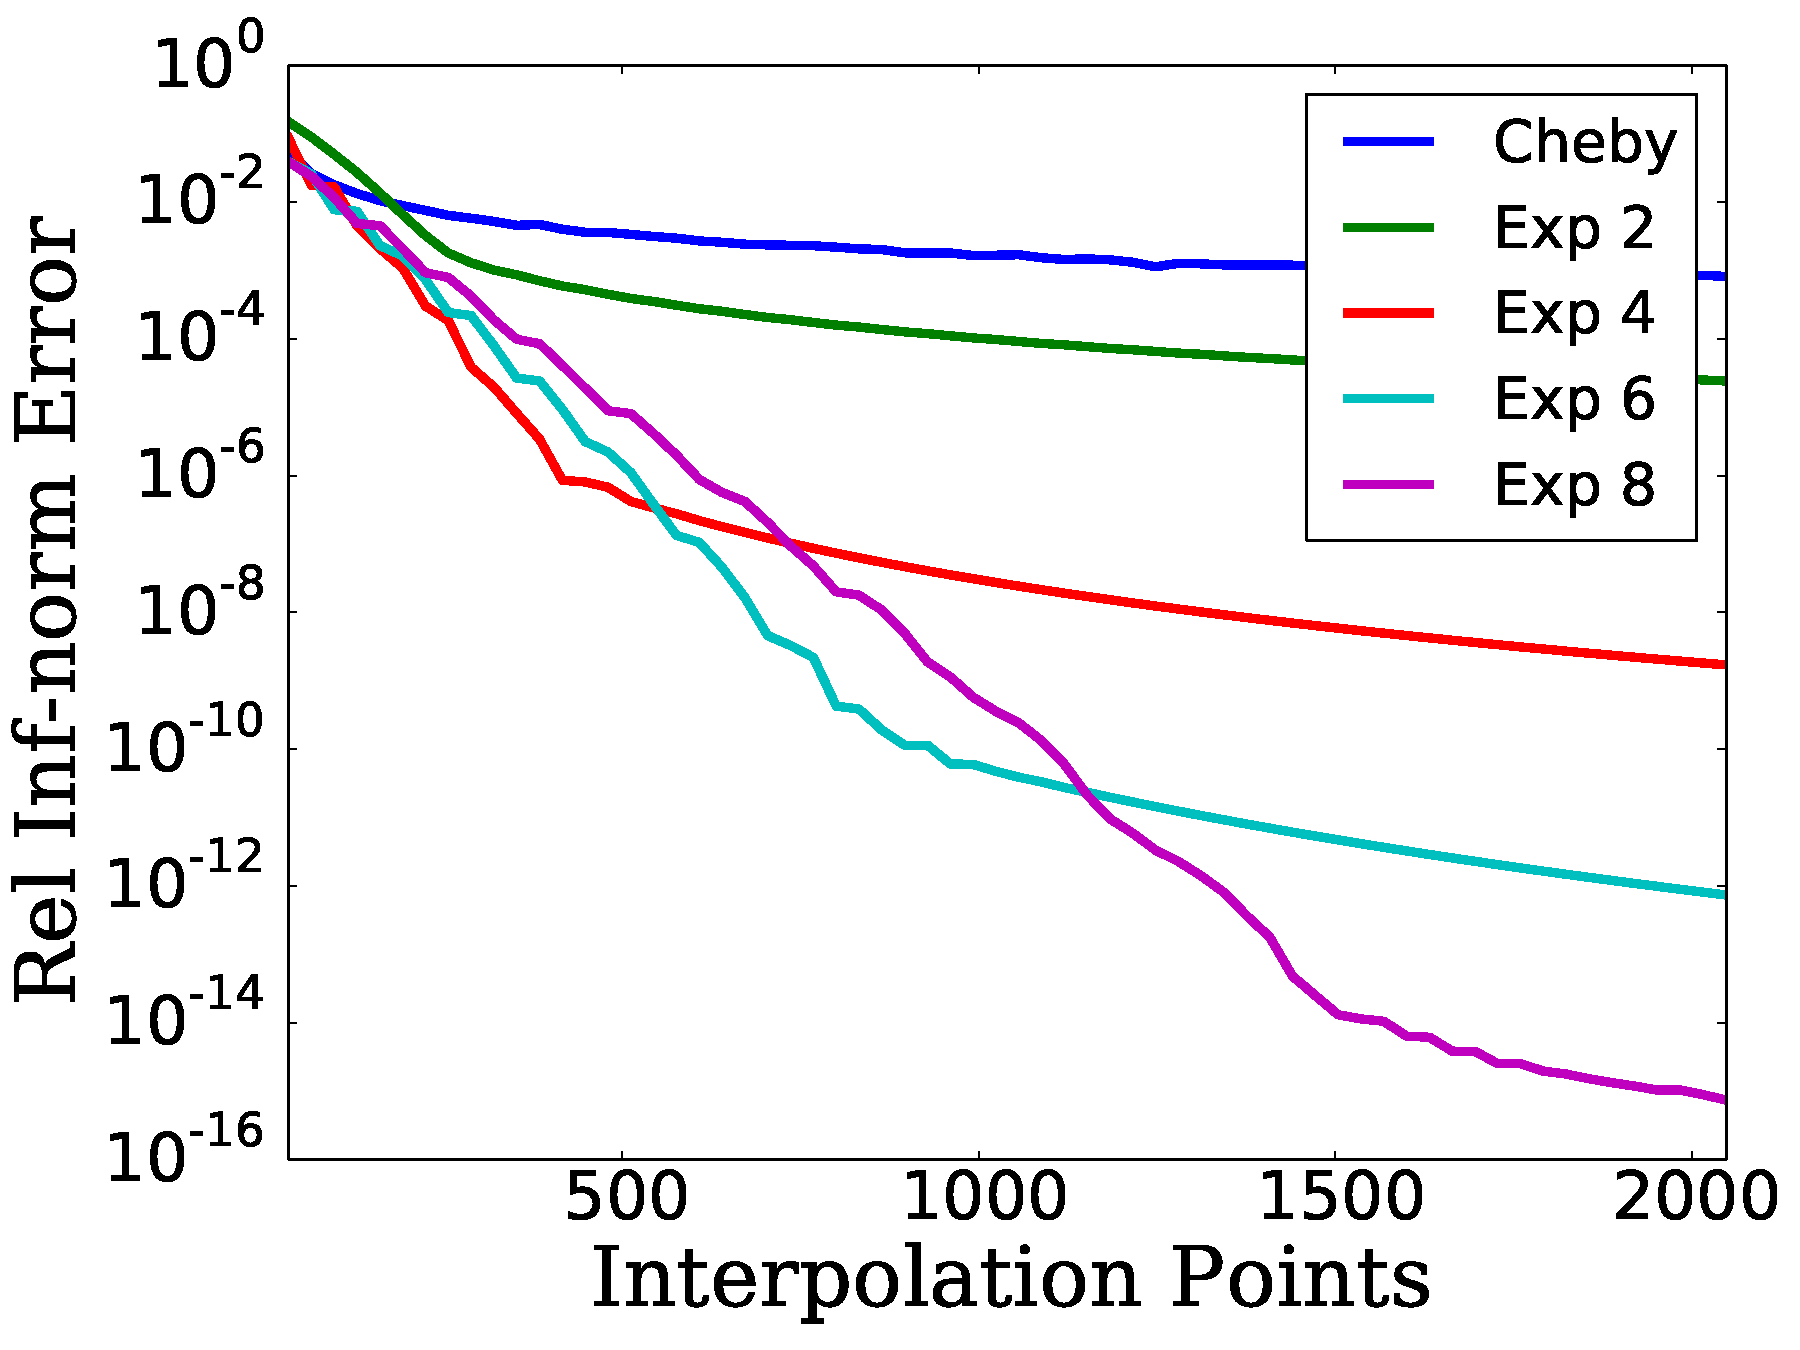
\includegraphics[width=\textwidth]{plots/cheby_interp_filter_2_rough_heaviside_2.pdf}
    \caption{Filters, Plot 2}
    \end{subfigure}
\caption[Rough Interpolation Comparison: Heaviside Jump Function 2]{
MSN interpolation and Chebyshev filtering results of the Heaviside jump
function $H_{2}$ for various $s$ values and filters.
We include standard Chebyshev interpolant in both filter examples for reference.
}
\label{fig:rough_comparison_heaviside_2}
\end{figure}




% Print results for comparing MSN with Heaviside jump function

\begin{figure}[p]
    \centering
    \begin{subfigure}{0.45\textwidth}
    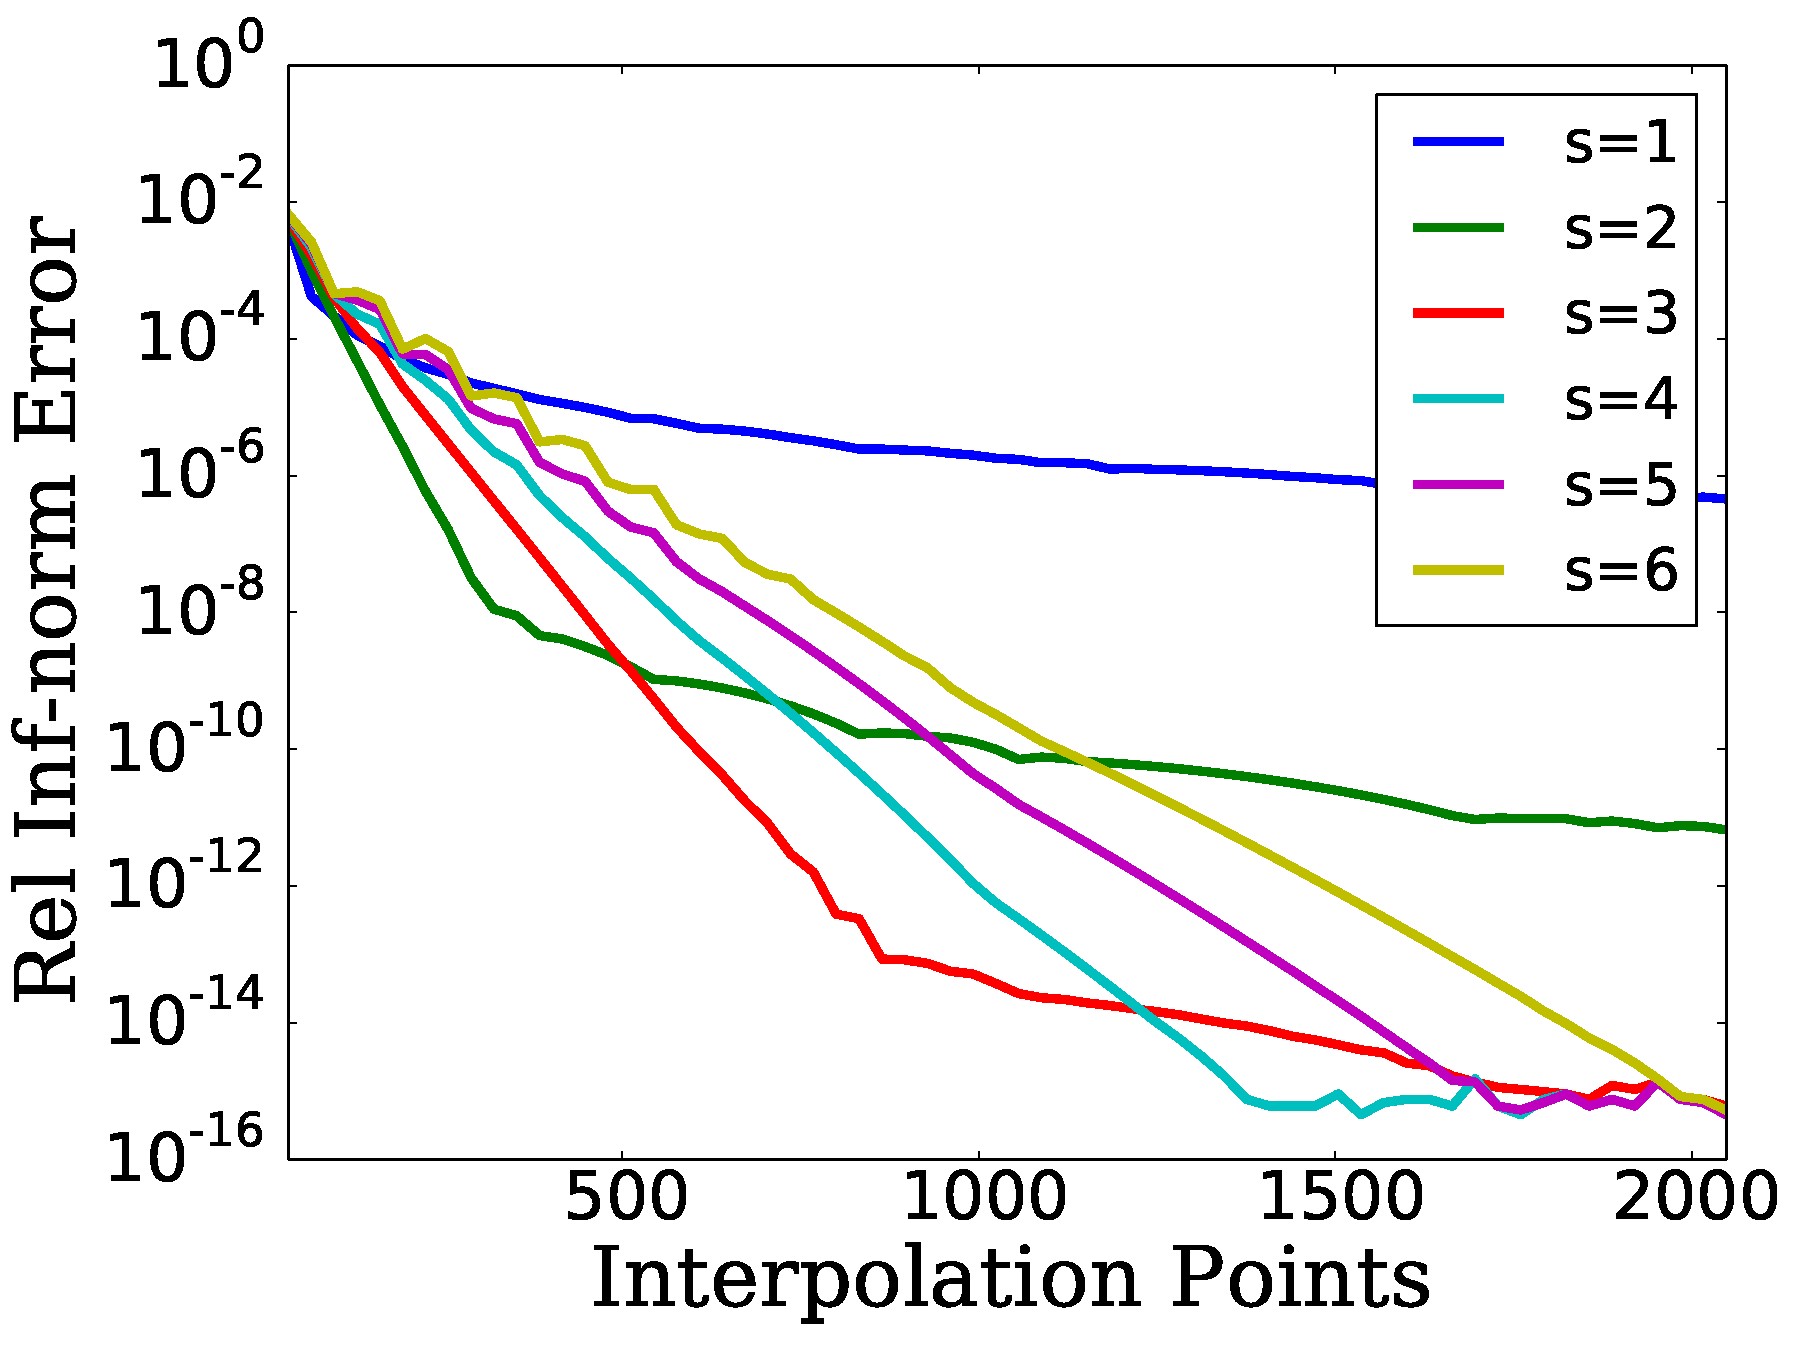
\includegraphics[width=\textwidth]{plots/msn_interp_fast_2n_rough_sharp_func_2.pdf}
    \caption{MSN Interpolation}
    \end{subfigure}

    \begin{subfigure}{0.45\textwidth}
    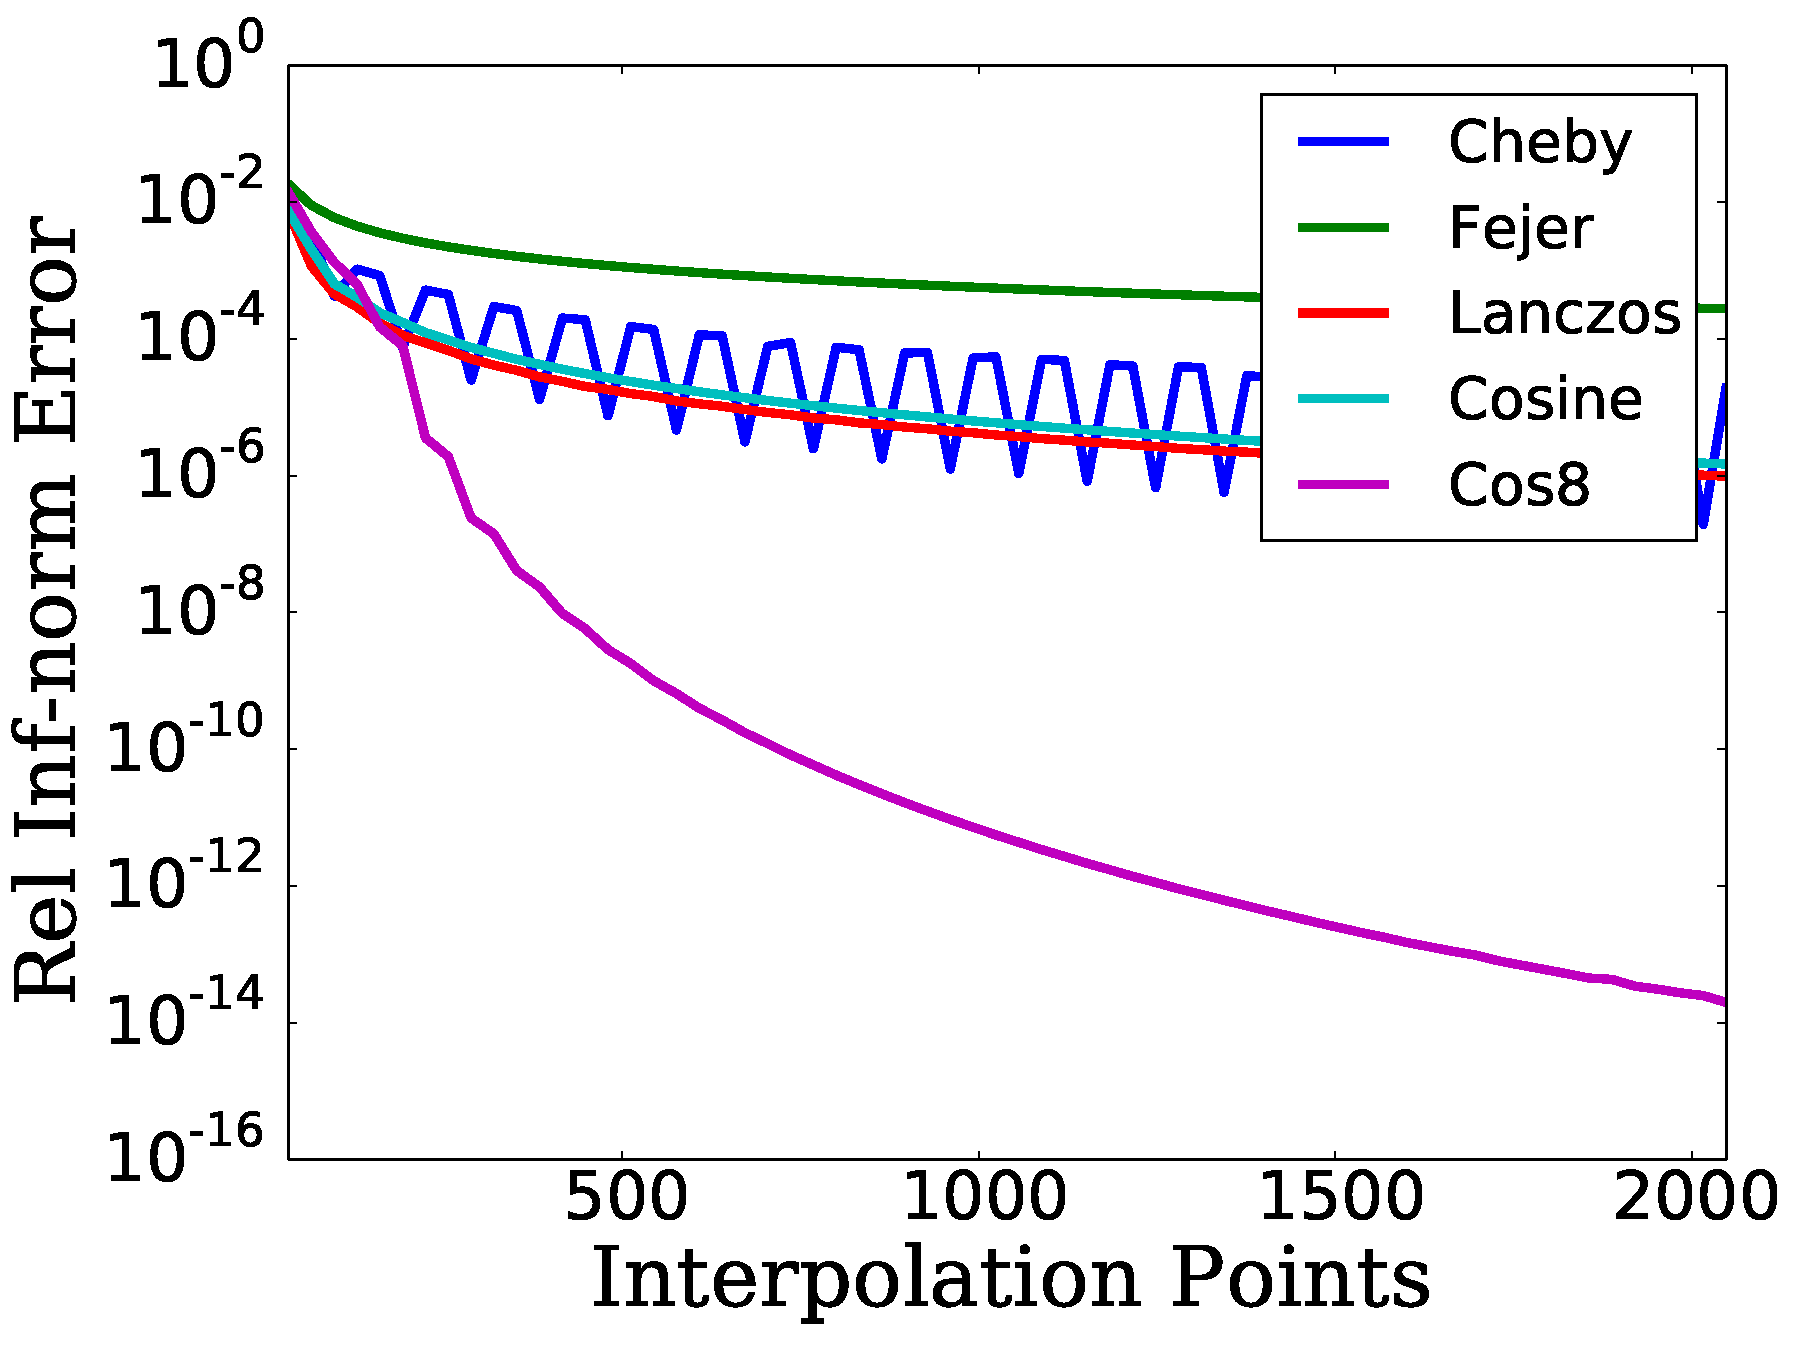
\includegraphics[width=\textwidth]{plots/cheby_interp_filter_rough_sharp_func_2.pdf}
    \caption{Filters, Plot 1}
    \end{subfigure}
    \begin{subfigure}{0.45\textwidth}
    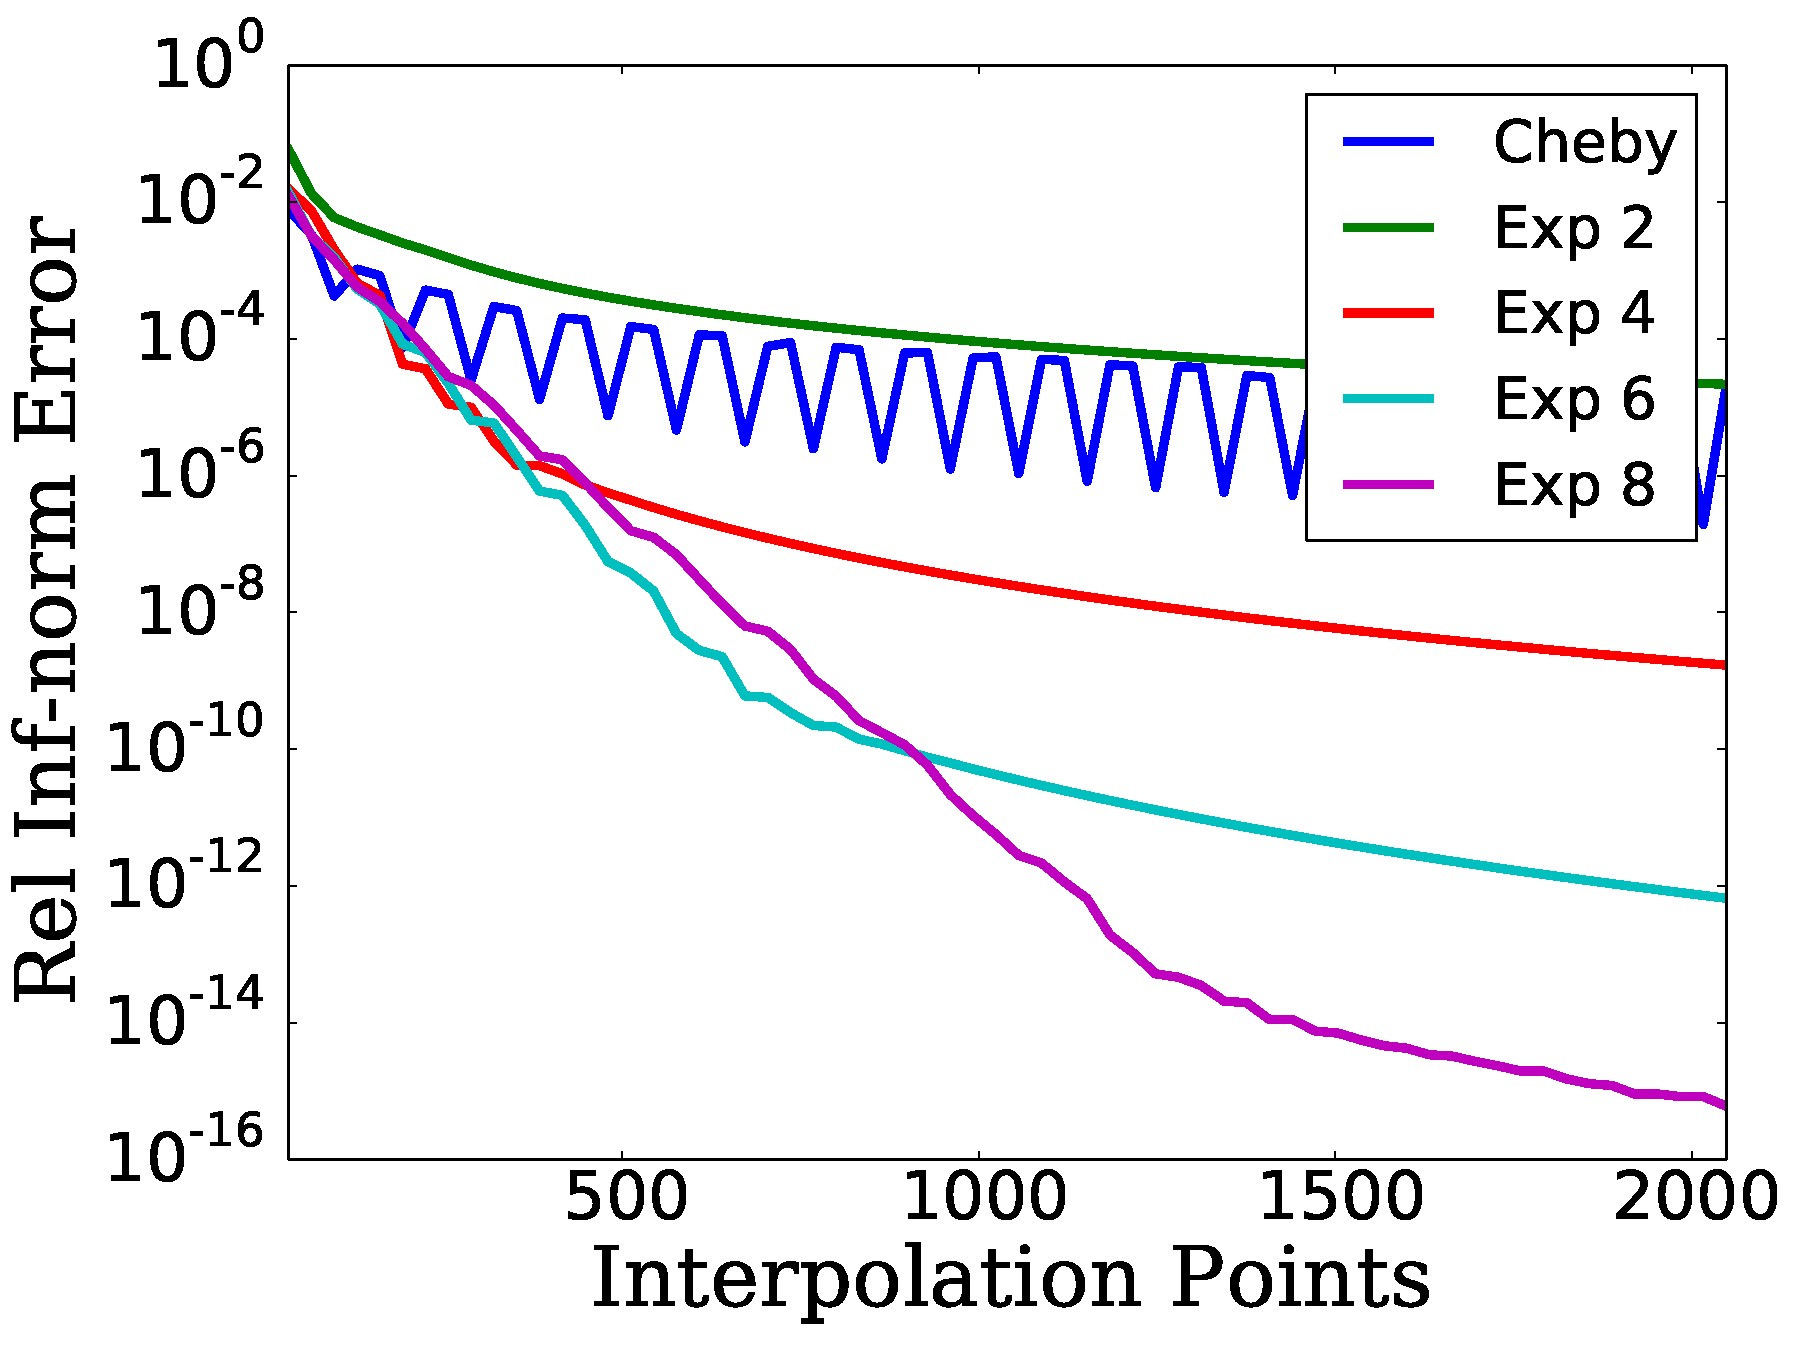
\includegraphics[width=\textwidth]{plots/cheby_interp_filter_2_rough_sharp_func_2.pdf}
    \caption{Filters, Plot 2}
    \end{subfigure}
\caption[Rough Interpolation Comparison: Sharp Function 2]{
MSN interpolation and Chebyshev filtering results of the Sharp Function
$G_{2}(\cdot,0.5)$ for various $s$ values and filters.
We include standard Chebyshev interpolant in both filter examples for reference.
}
\label{fig:rough_comparison_sharp_func_2}
\end{figure}




% Print results for comparing MSN with Heaviside jump function

\begin{figure}[p]
    \centering
    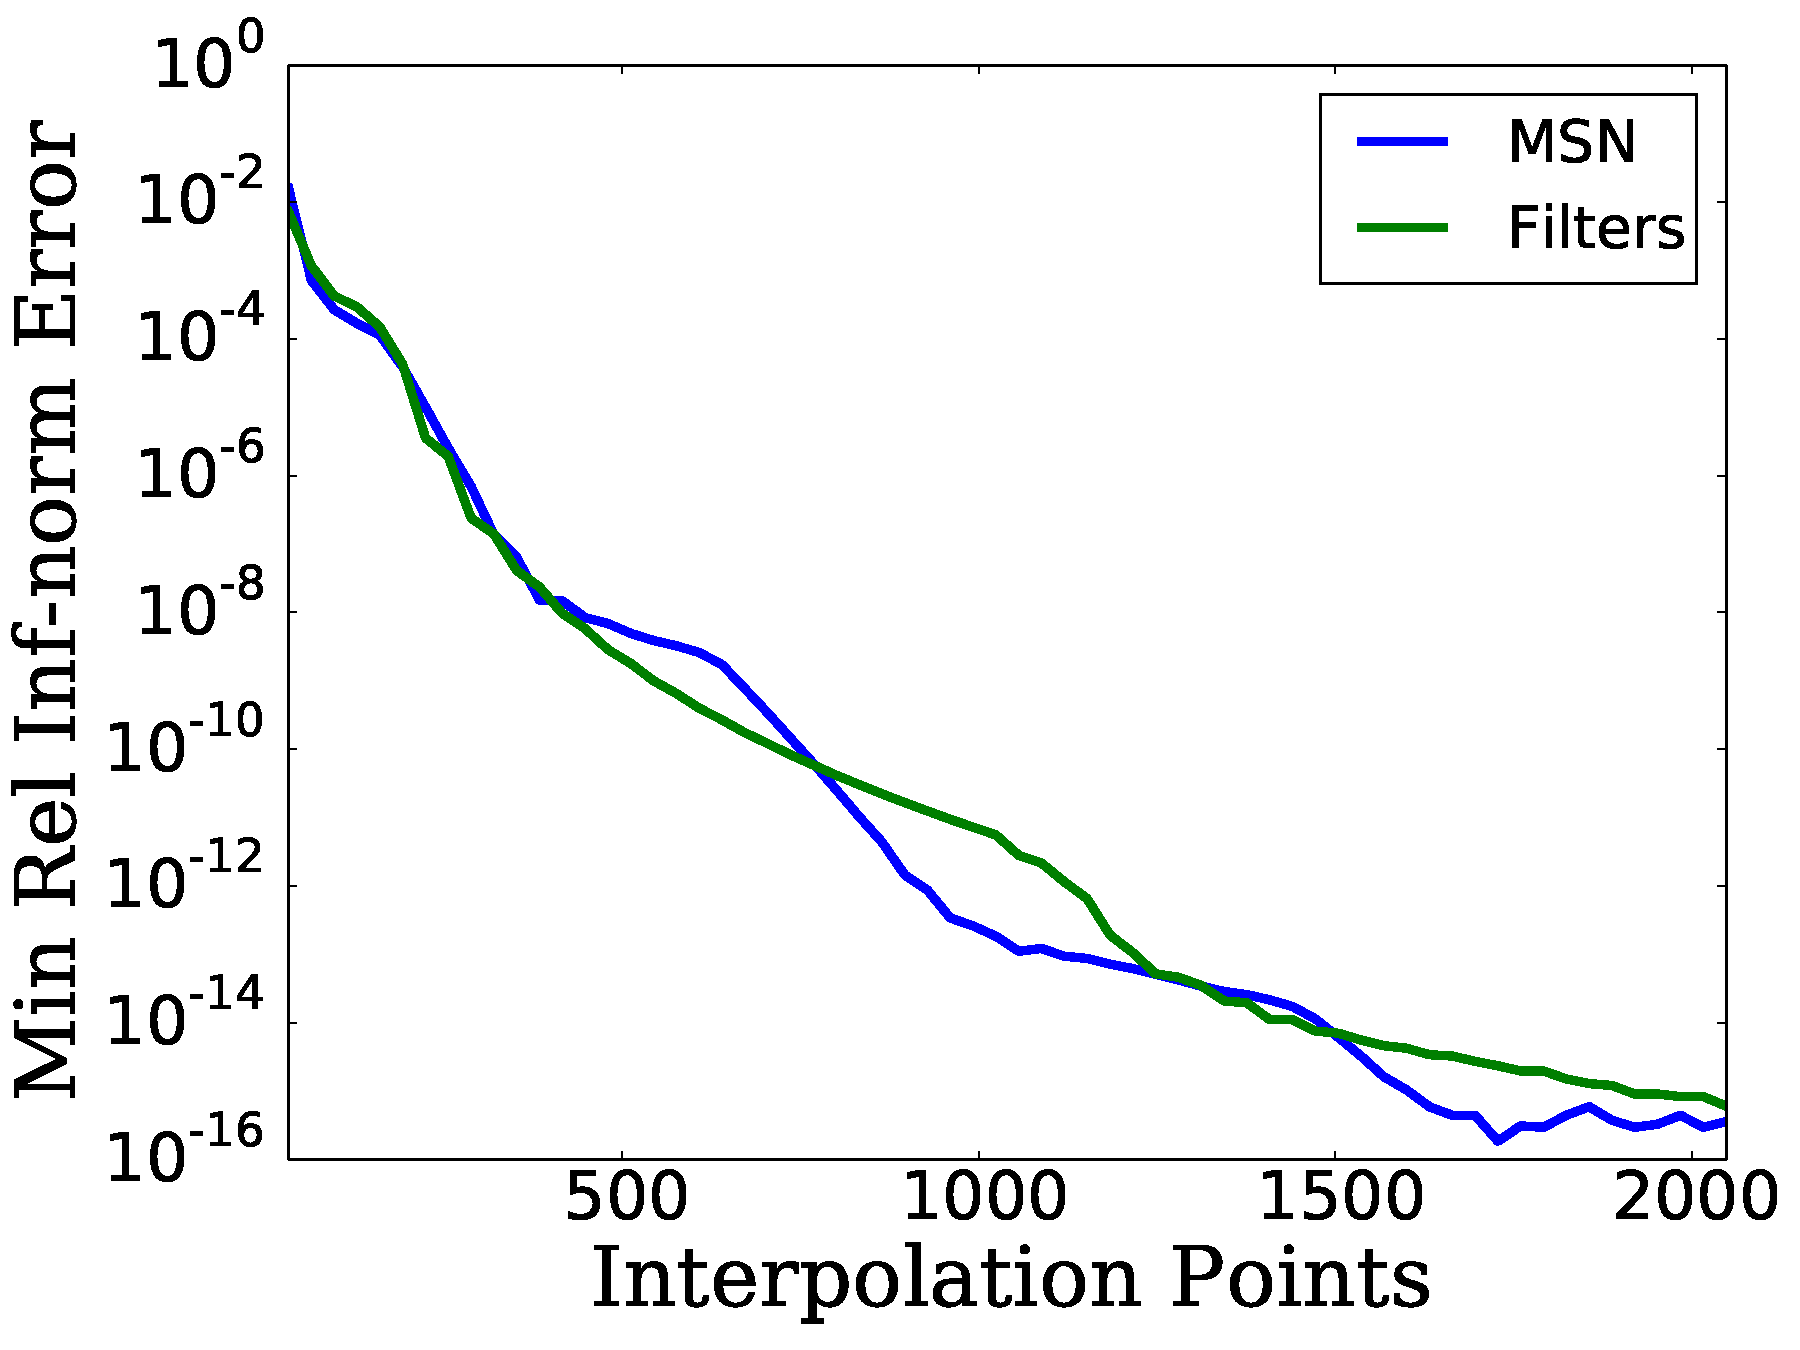
\includegraphics[width=0.9\textwidth]{plots/msn_filter_comp_heaviside_2.pdf}
    \caption[Best MSN vs.~Best Filter Comparison: Heaviside Jump Function 2]{
    We plot the minimum MSN interpolation error and compare it
    to the minimum filter error over all Chebshev filters.
    These error results are from attempting to approximate $H_{2}$.
    }
\label{fig:msn_filter_comp_heaviside_2}
\end{figure}




% Print results for comparing MSN with Heaviside jump function

\begin{figure}[p]
    \centering
    \begin{subfigure}{0.45\textwidth}
    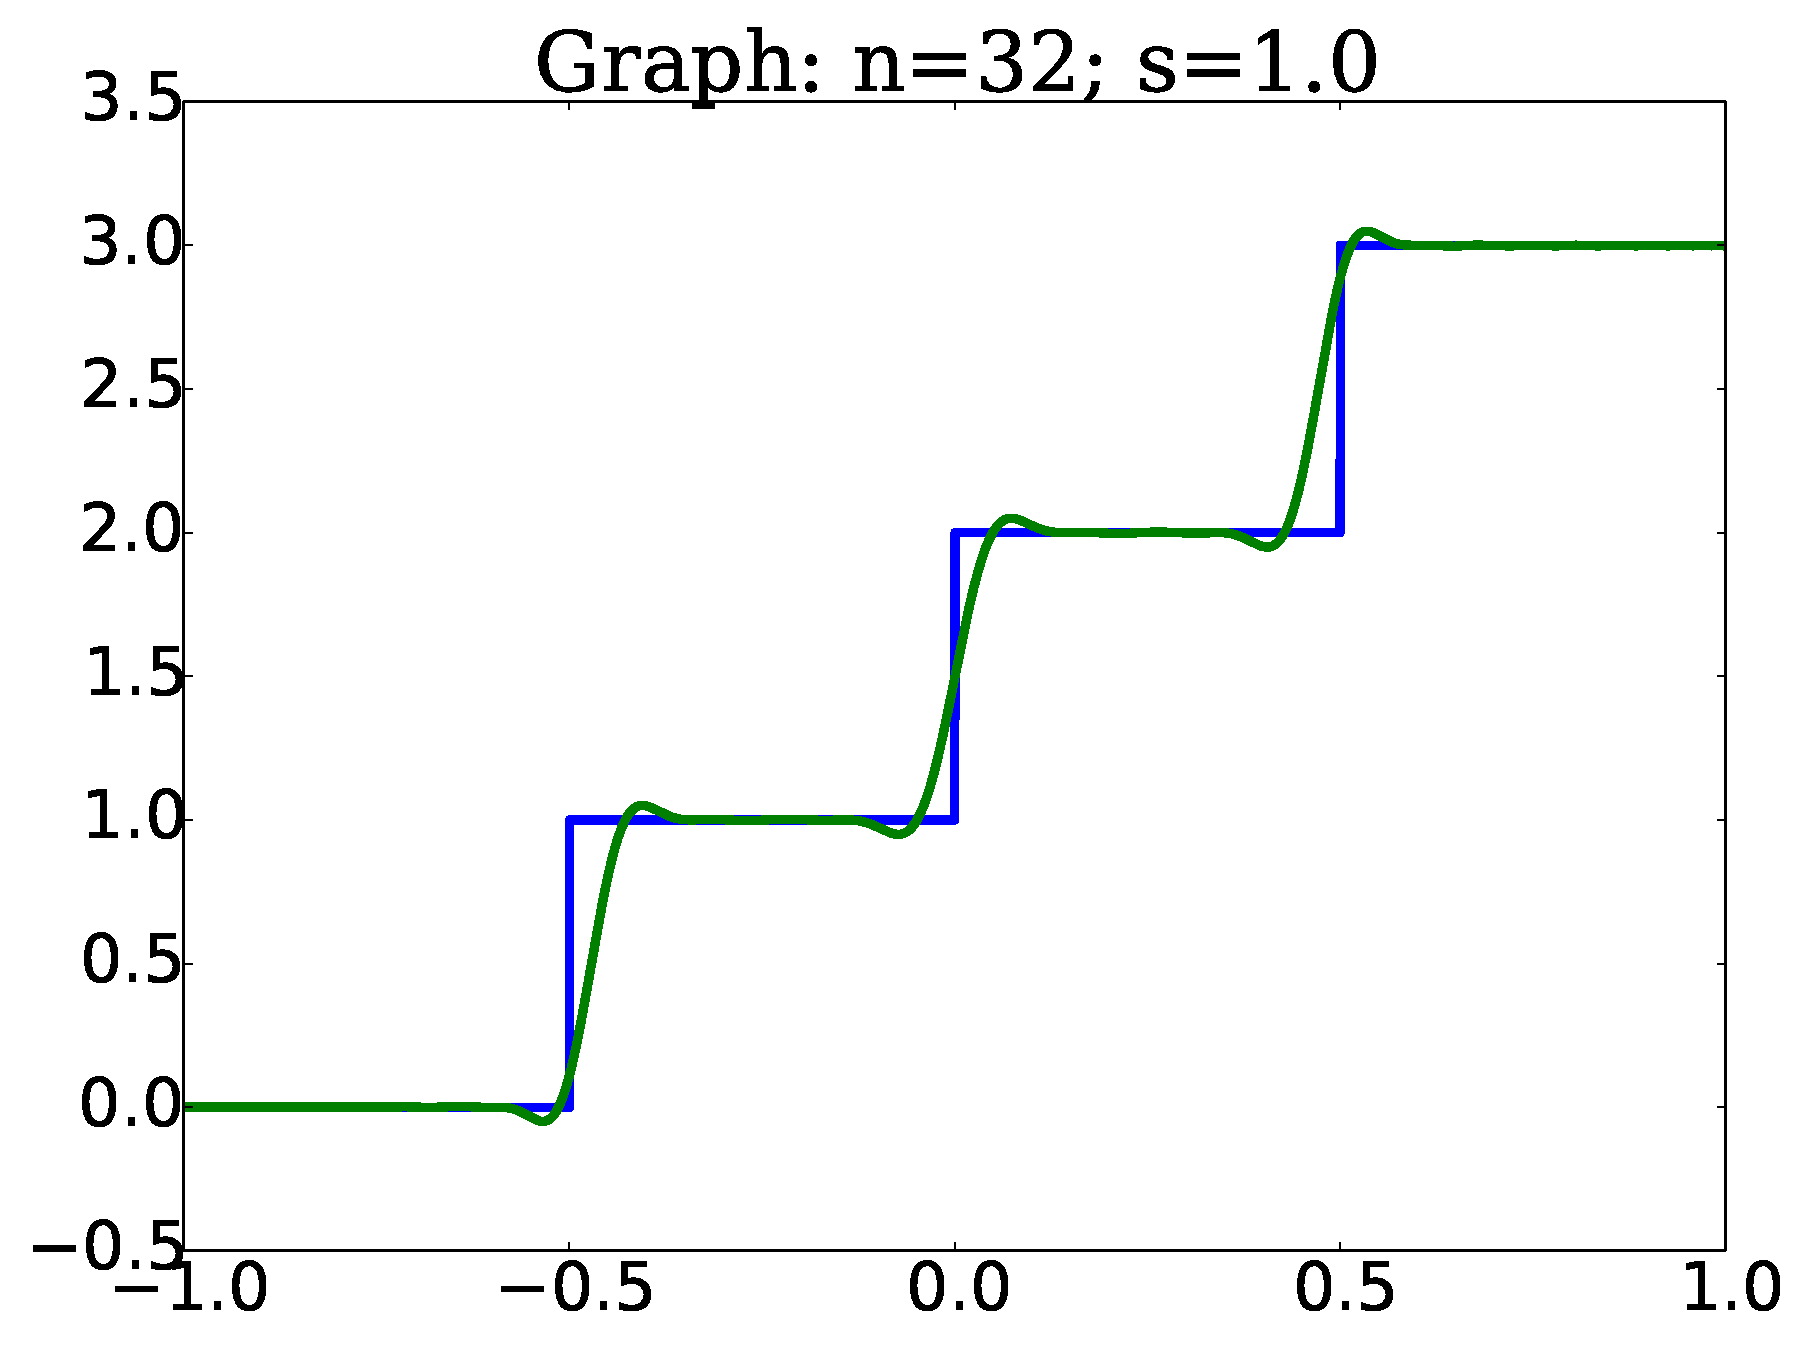
\includegraphics[width=\textwidth]{plots/graph_n_32_s_1_heaviside_2.pdf}
    \end{subfigure}
    \begin{subfigure}{0.45\textwidth}
    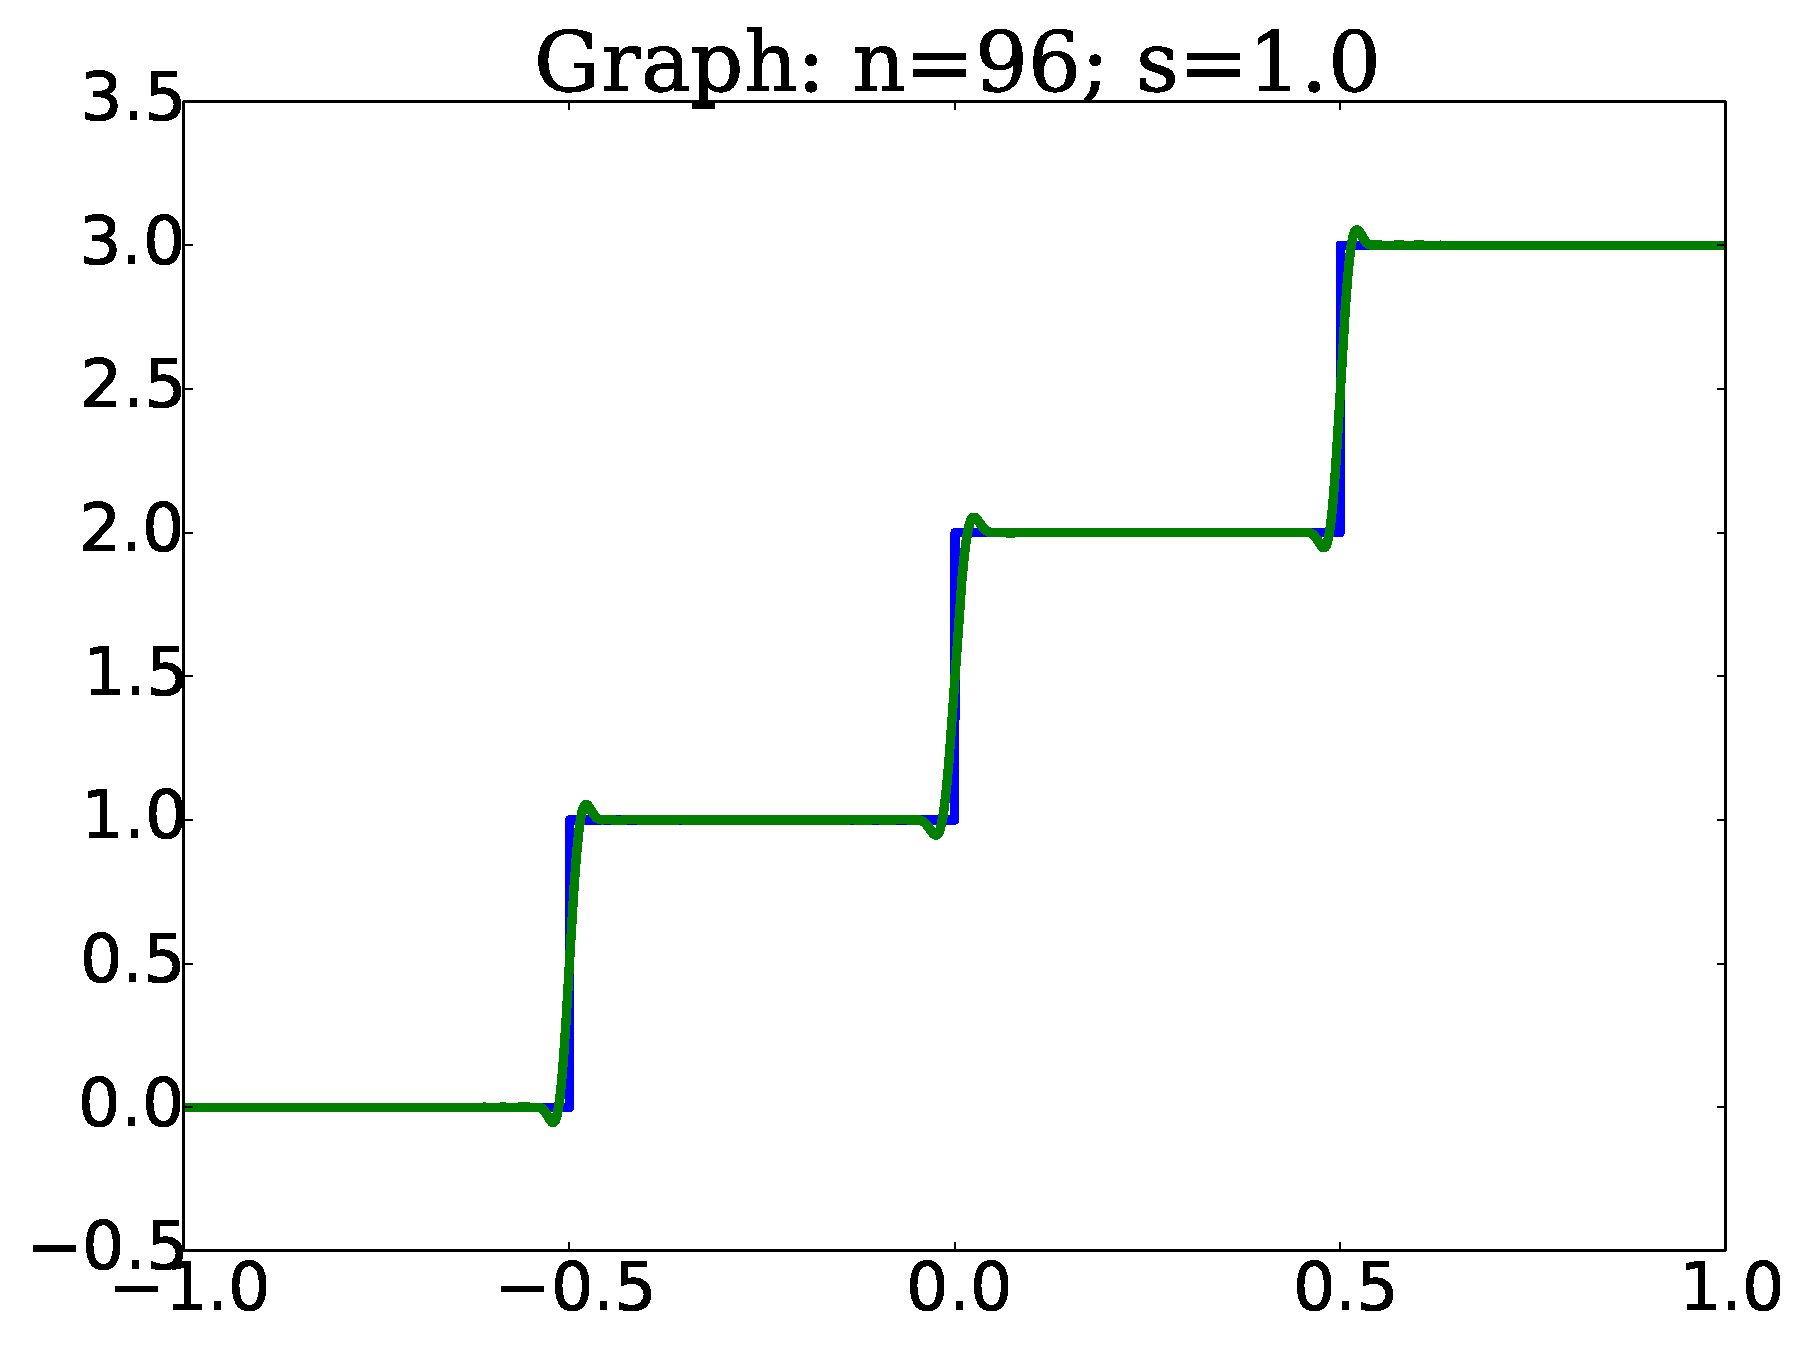
\includegraphics[width=\textwidth]{plots/graph_n_96_s_1_heaviside_2.pdf}
    \end{subfigure}

    \begin{subfigure}{0.45\textwidth}
    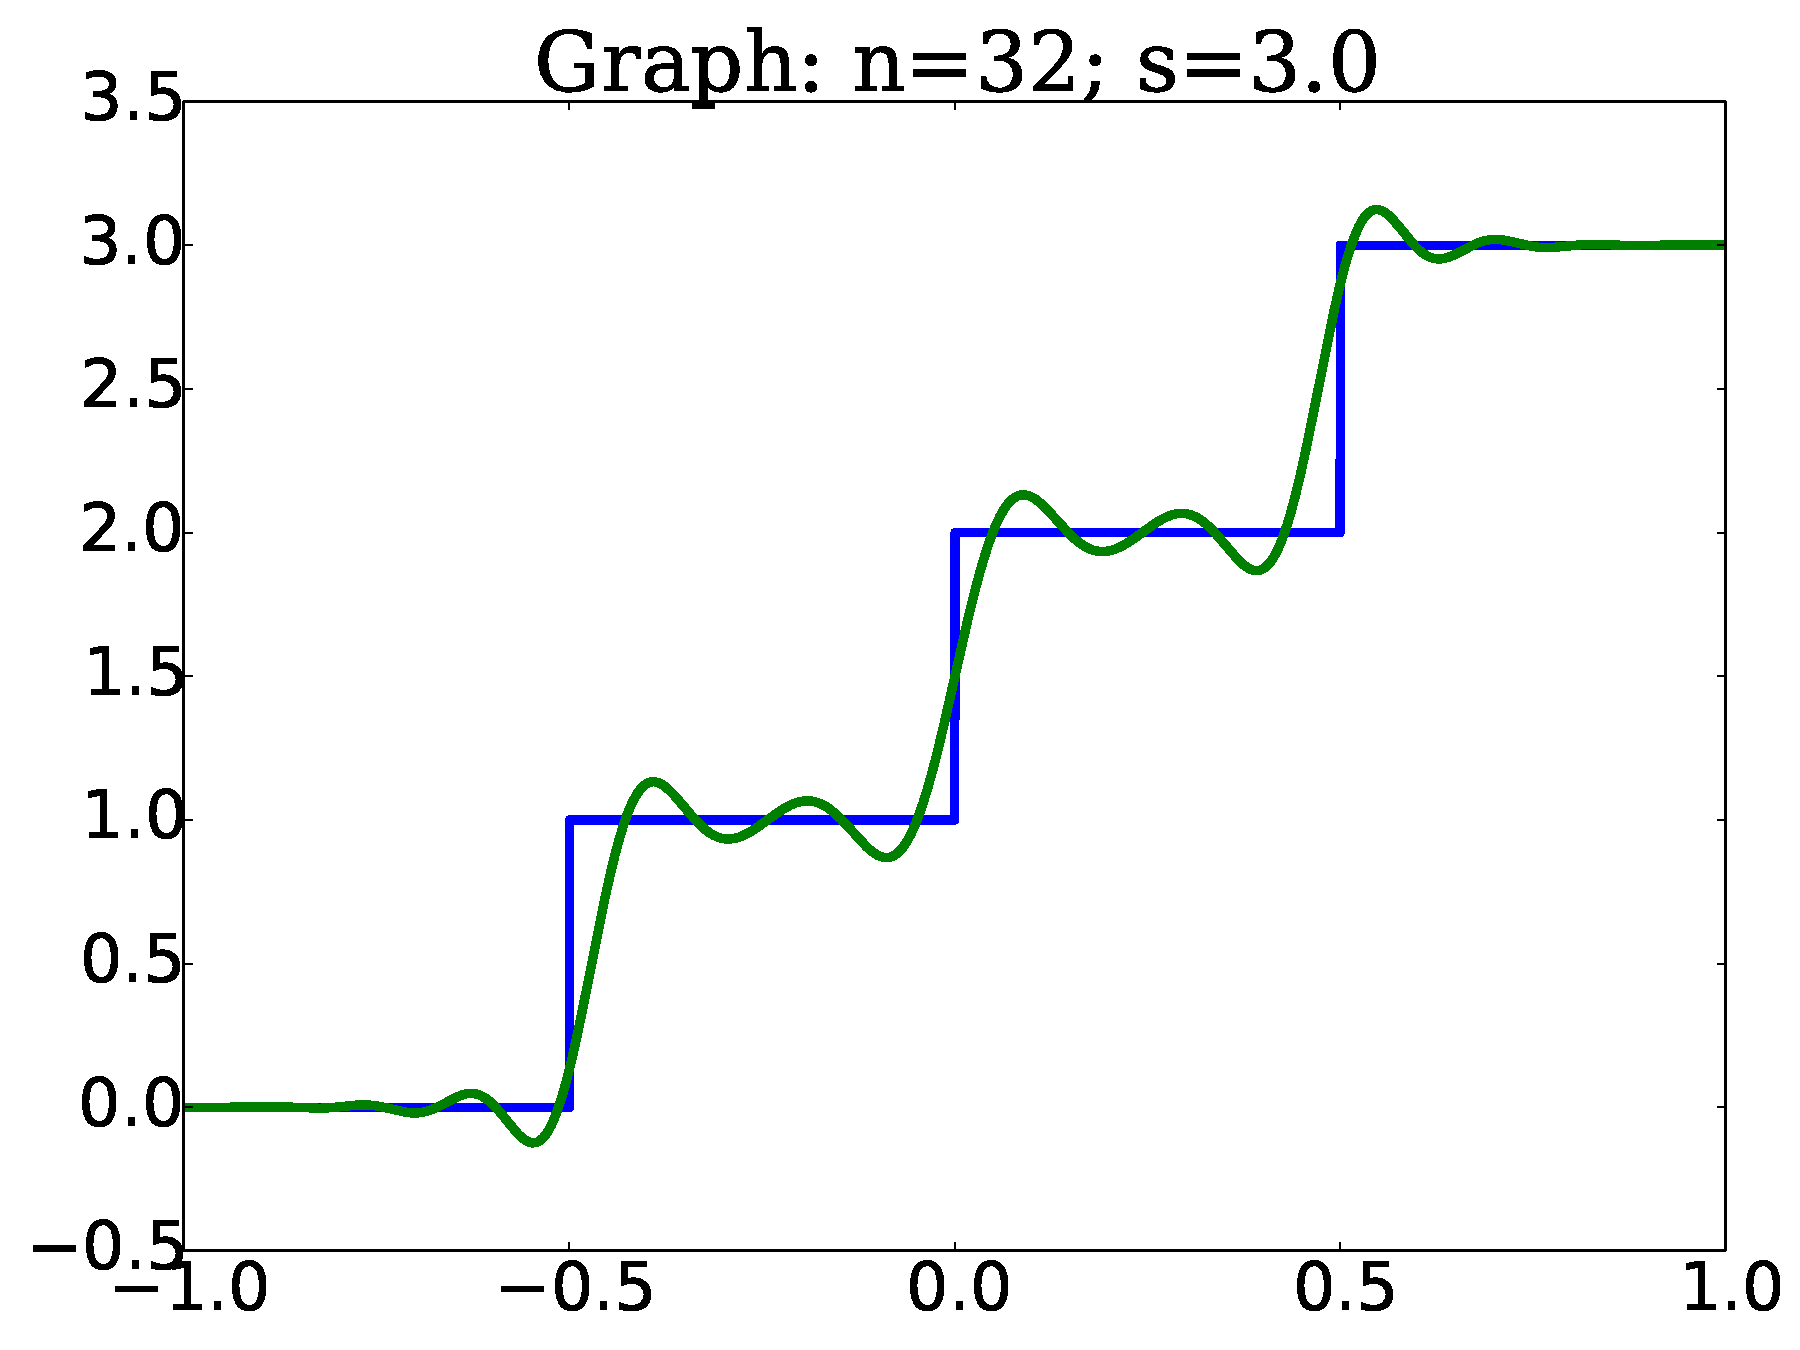
\includegraphics[width=\textwidth]{plots/graph_n_32_s_3_heaviside_2.pdf}
    \end{subfigure}
    \begin{subfigure}{0.45\textwidth}
    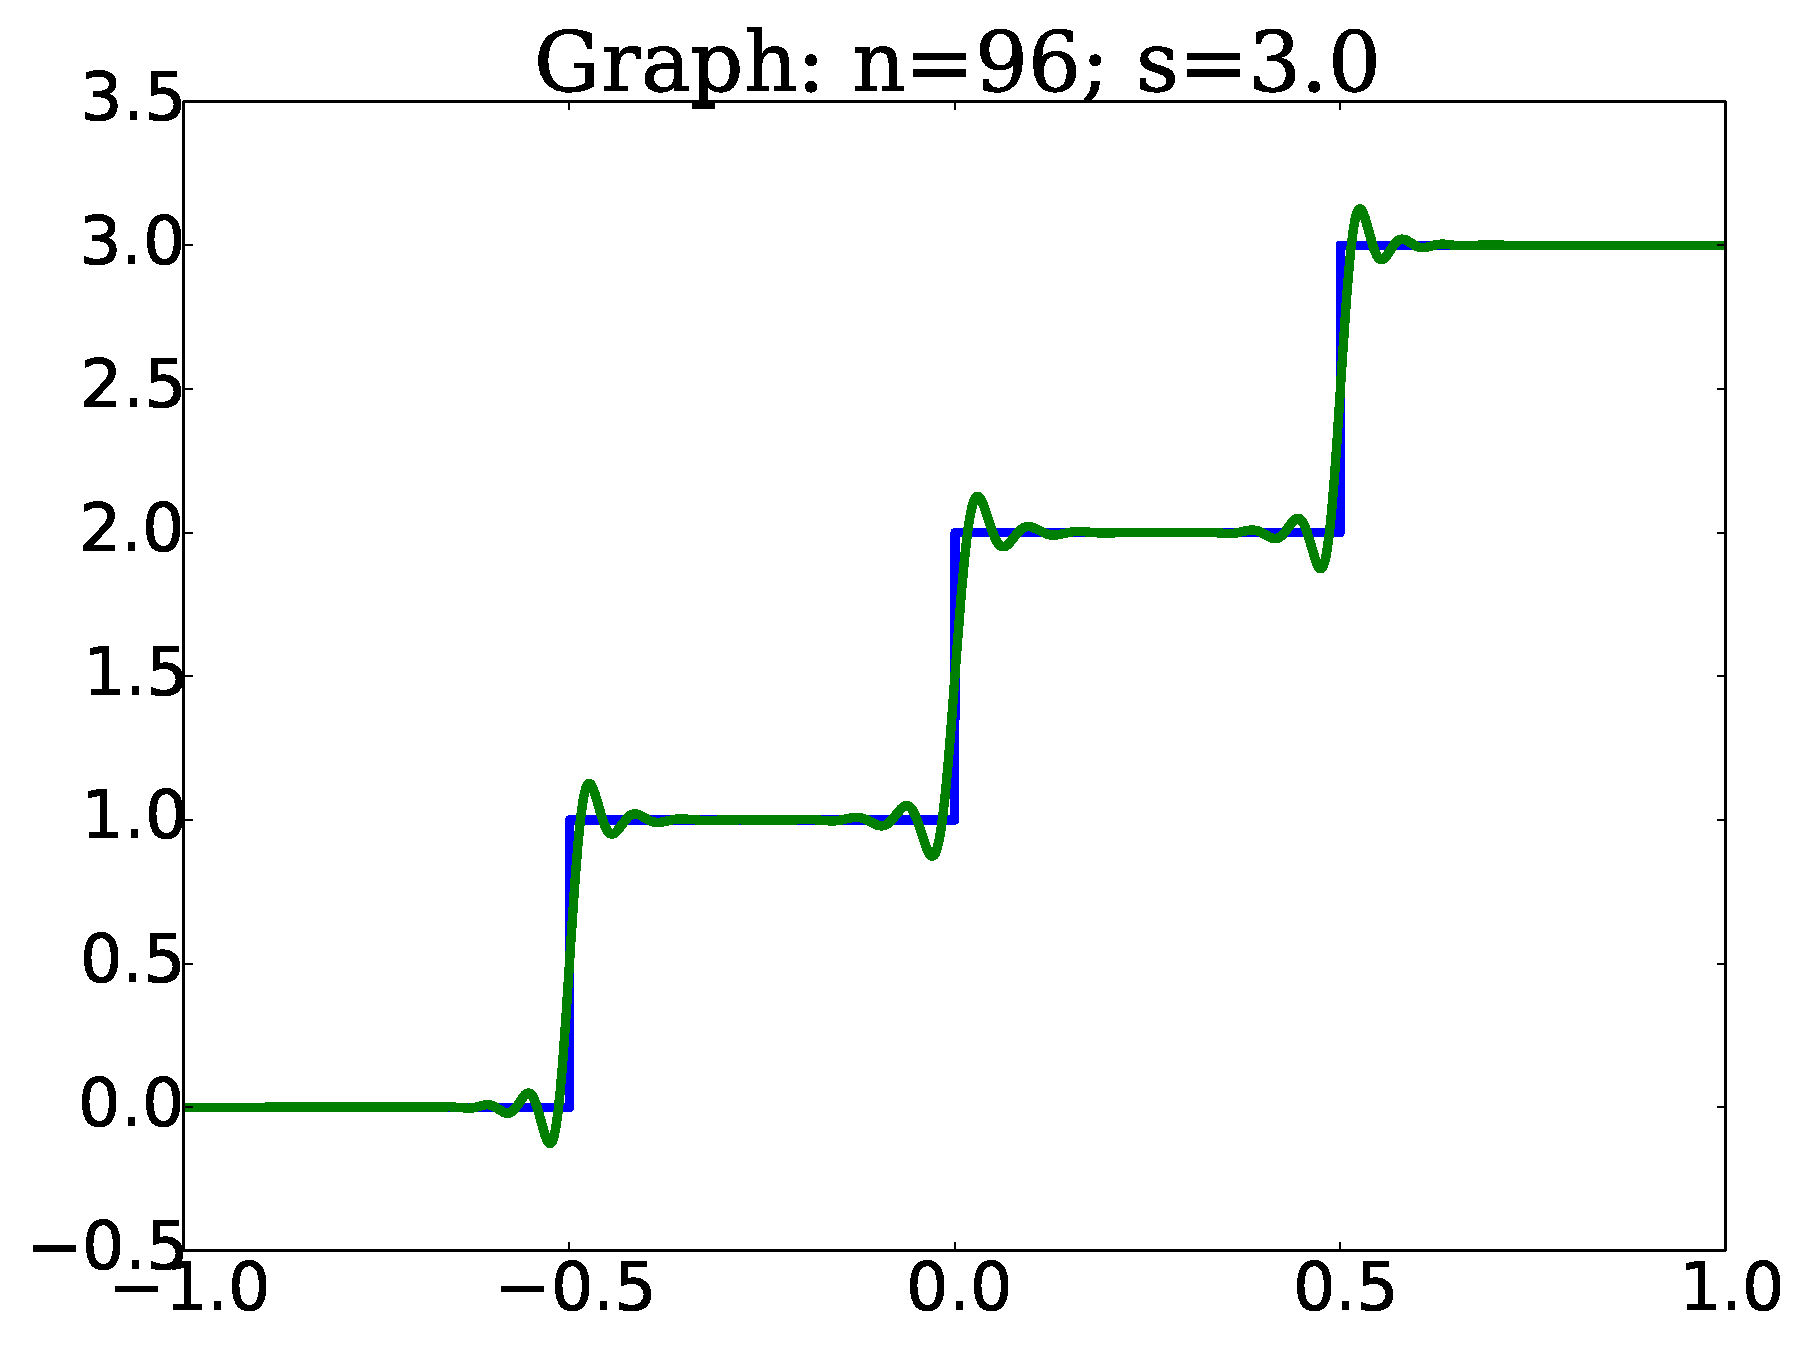
\includegraphics[width=\textwidth]{plots/graph_n_96_s_3_heaviside_2.pdf}
    \end{subfigure}

    \begin{subfigure}{0.45\textwidth}
    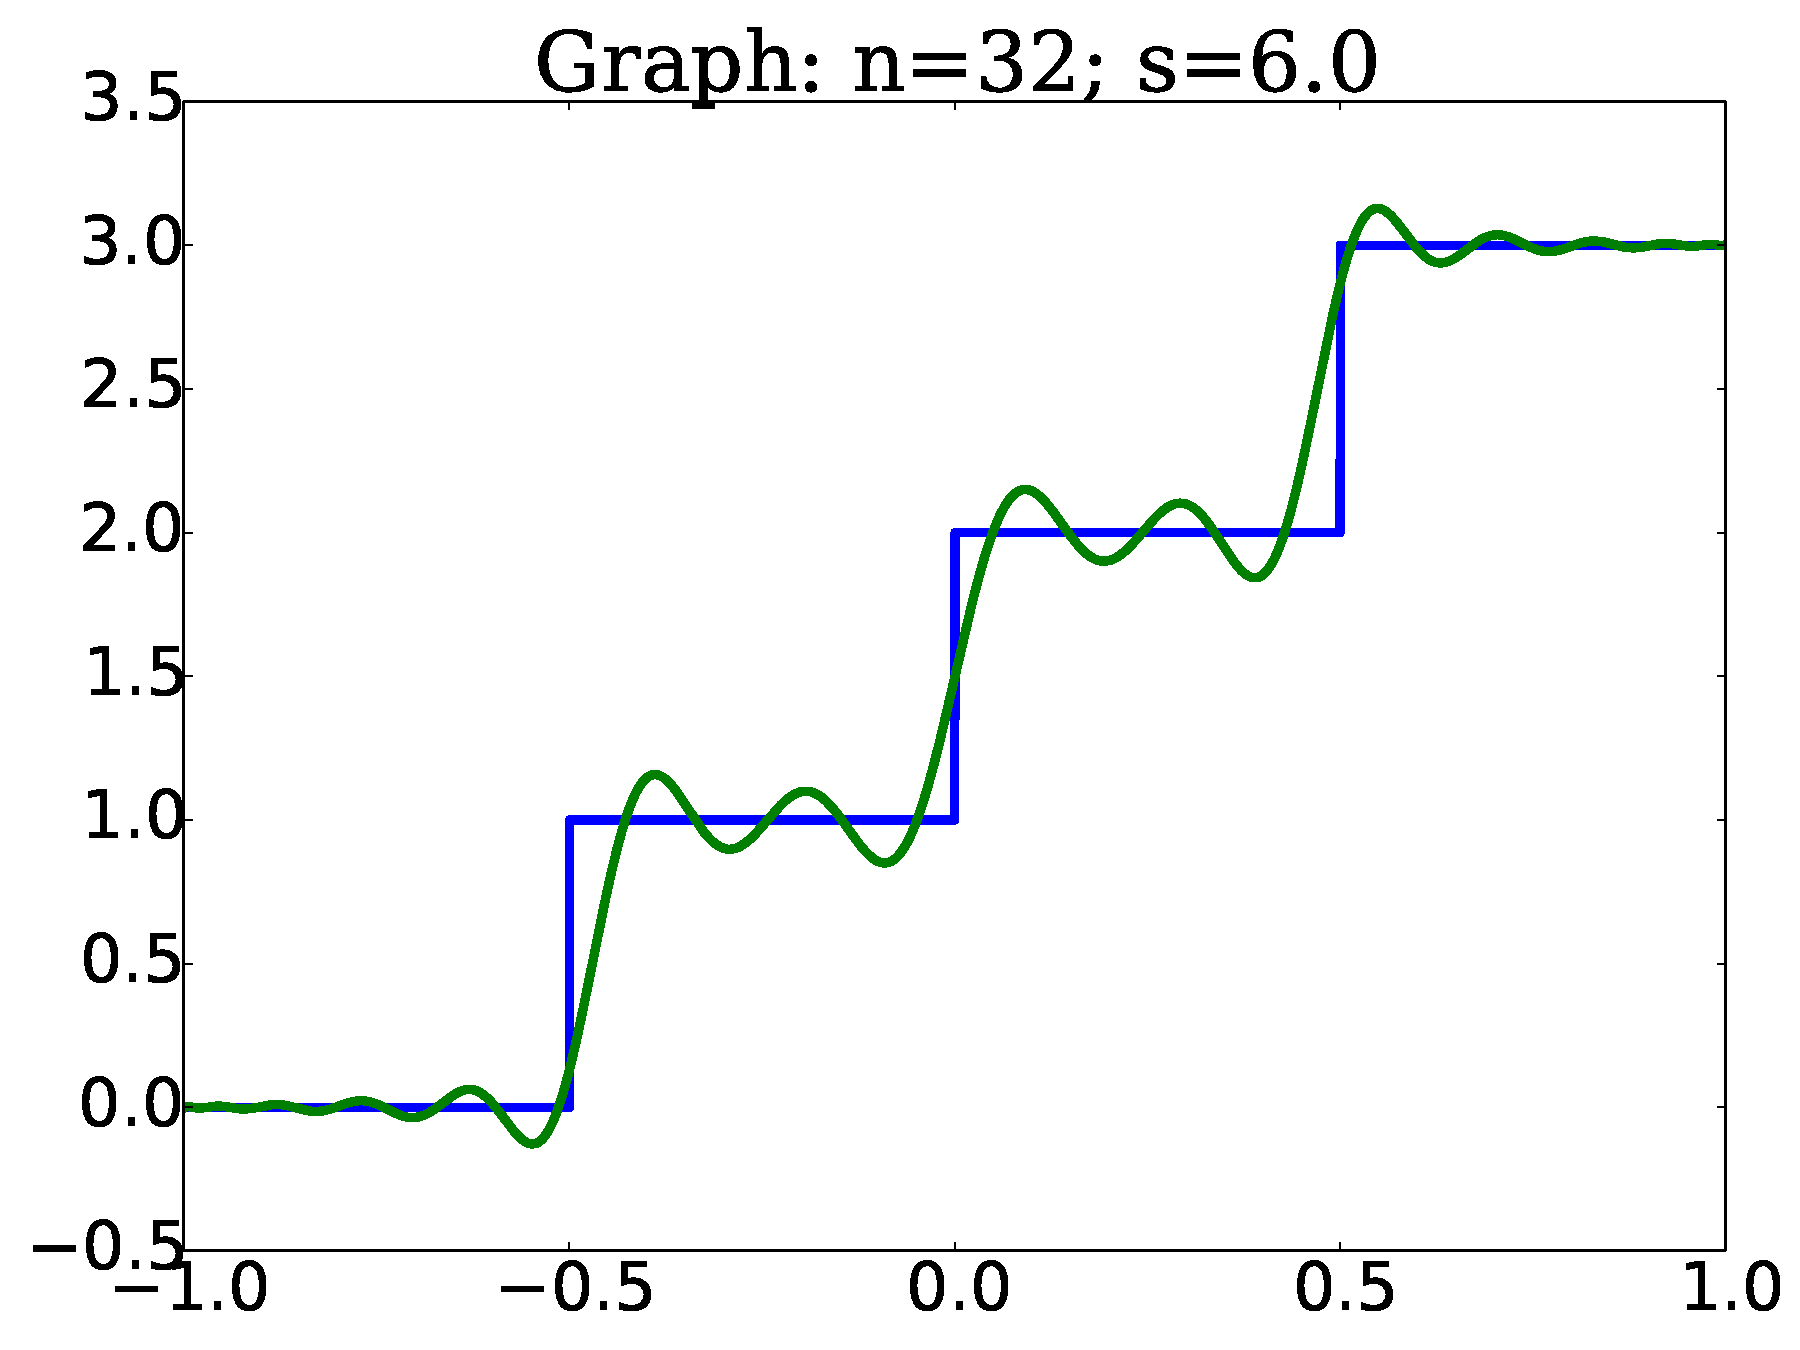
\includegraphics[width=\textwidth]{plots/graph_n_32_s_6_heaviside_2.pdf}
    \end{subfigure}
    \begin{subfigure}{0.45\textwidth}
    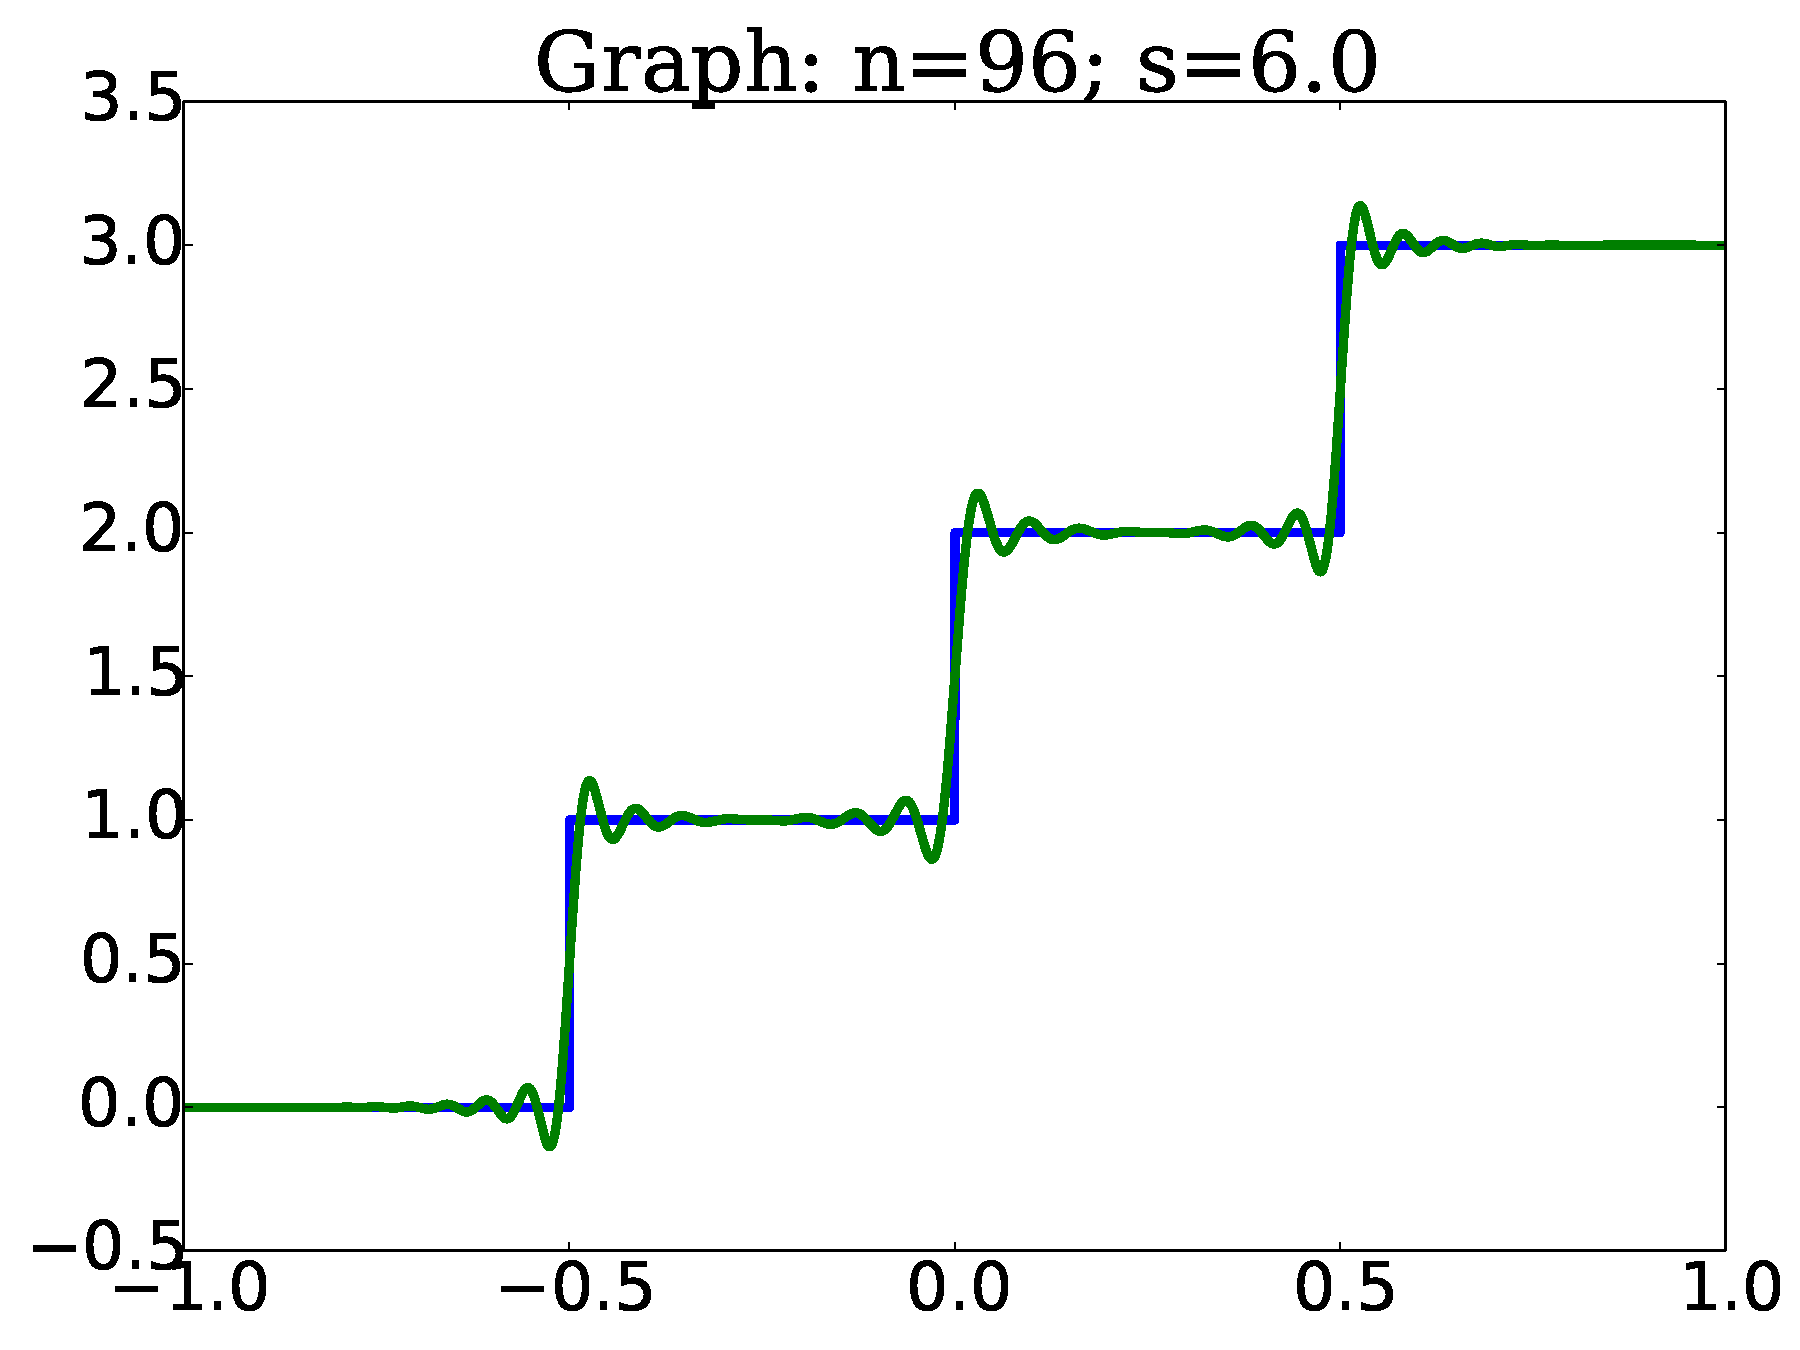
\includegraphics[width=\textwidth]{plots/graph_n_96_s_6_heaviside_2.pdf}
    \end{subfigure}
\caption[Example Plots of MSN Interpolation of Rough Functions]{
We plot MSN approximations against the true solution $H_{2}$
for various $s$ and $n$ values.
}
\label{fig:msn_n_s_heaviside_2}
\end{figure}




% Print results for comparing MSN with Heaviside jump function

\begin{figure}[p]
    \centering
    \begin{subfigure}{0.45\textwidth}
    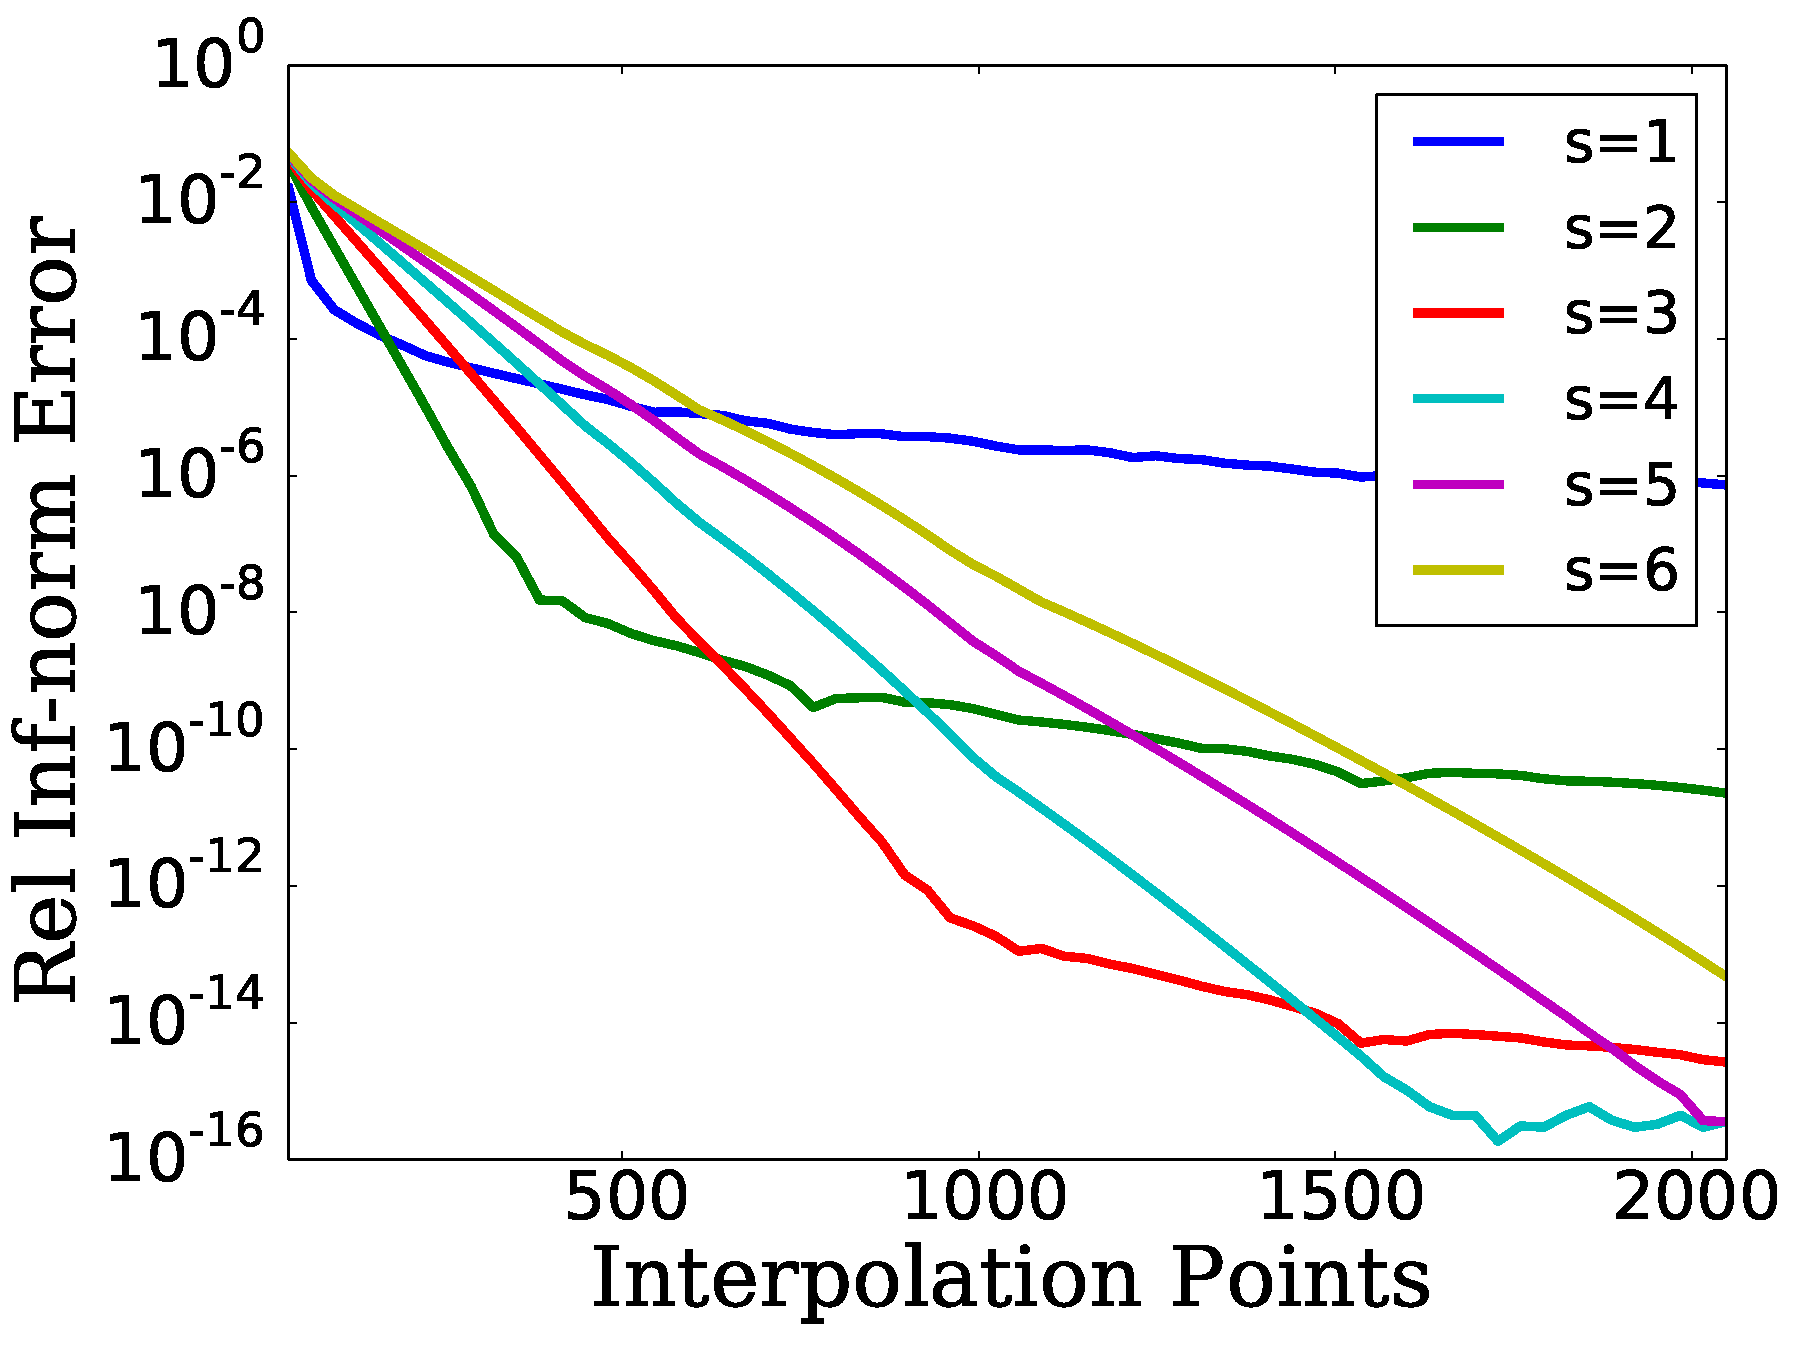
\includegraphics[width=\textwidth]{plots/msn_interp_fast_2n_rough_heaviside_2.pdf}
    \caption{Degree $2n$}
    \end{subfigure}
    \begin{subfigure}{0.45\textwidth}
    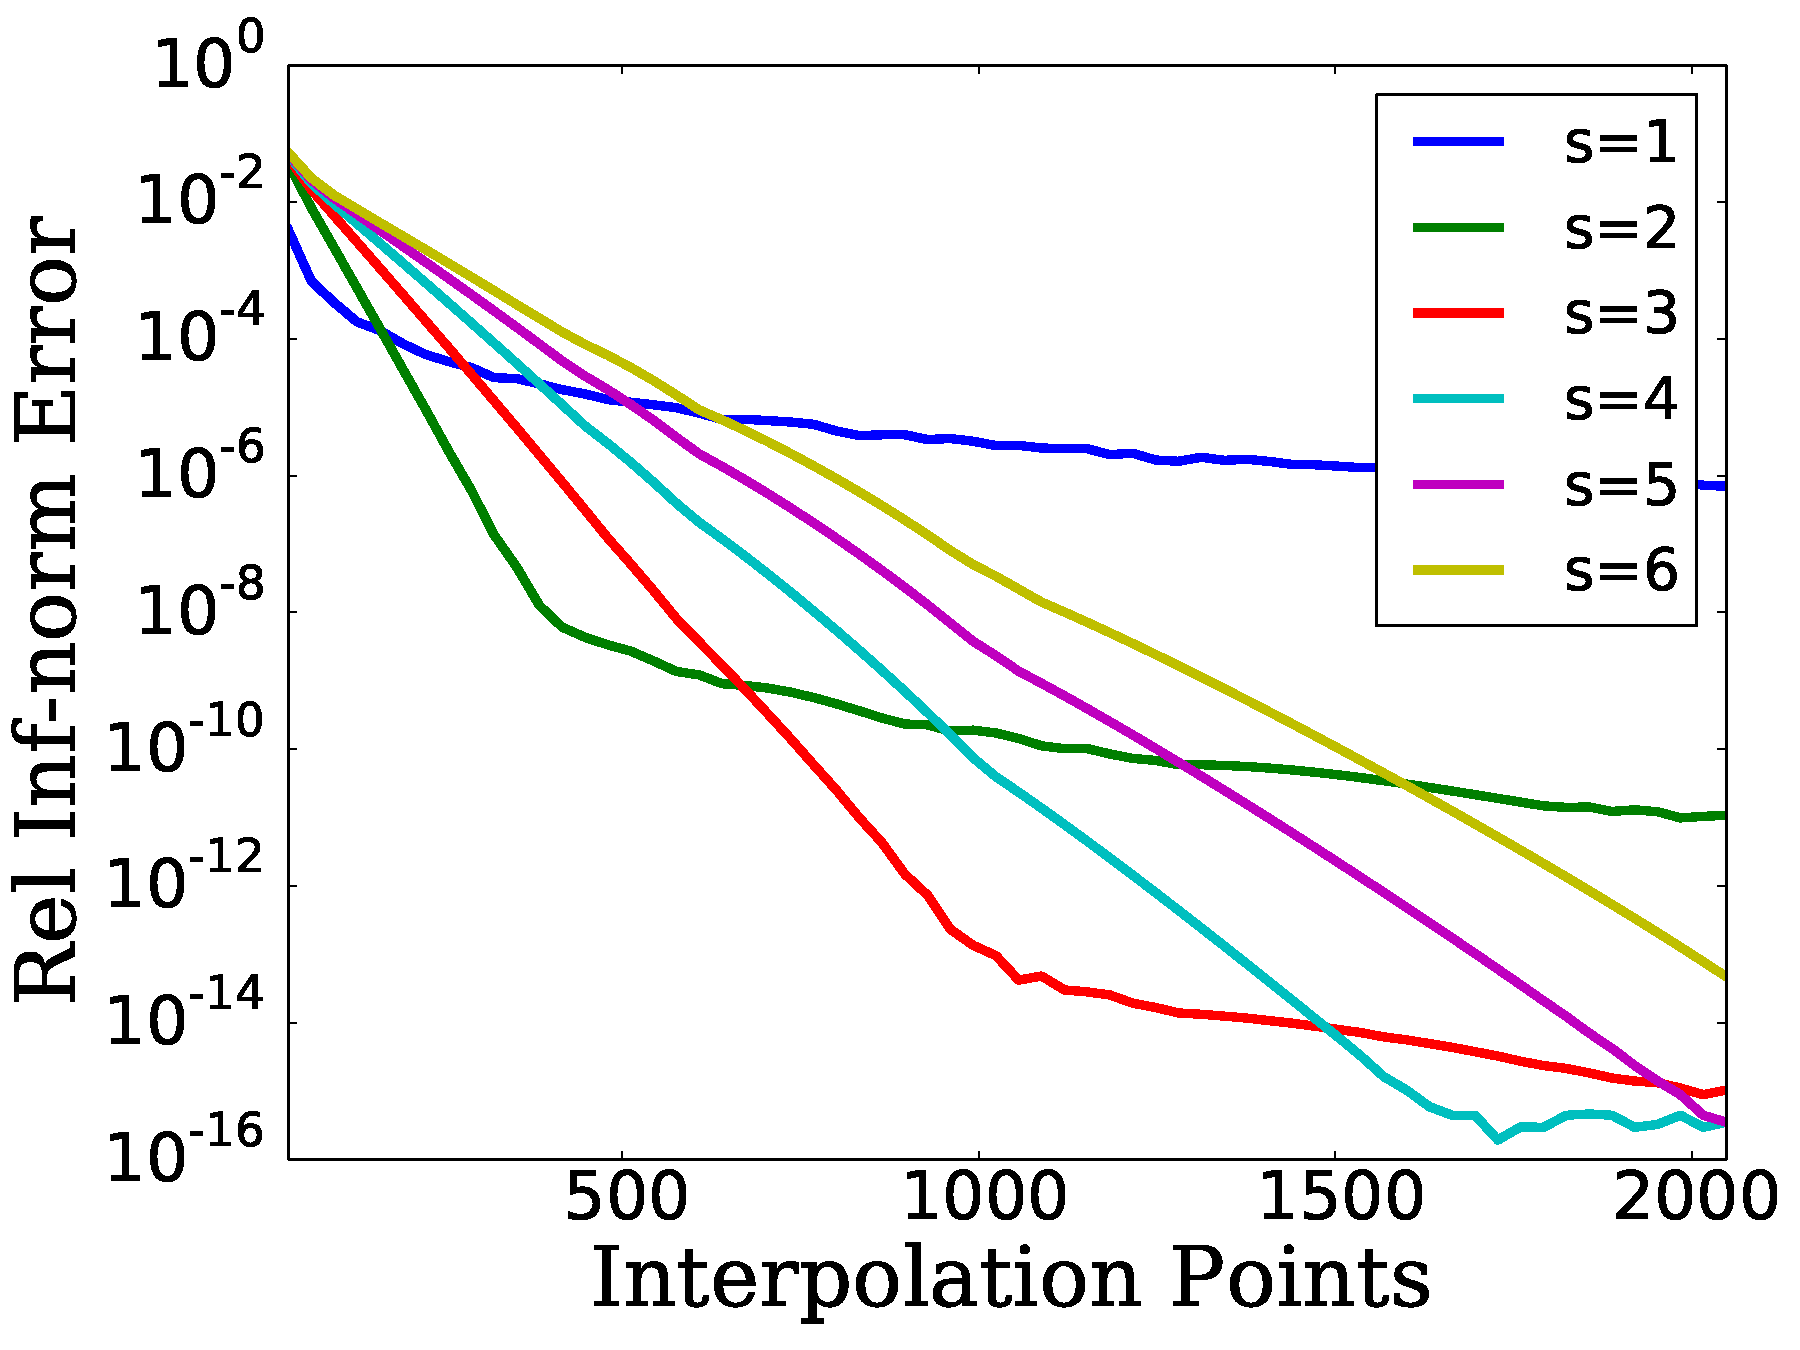
\includegraphics[width=\textwidth]{plots/msn_interp_fast_4n_rough_heaviside_2.pdf}
    \caption{Degree $4n$}
    \end{subfigure}

    \begin{subfigure}{0.45\textwidth}
    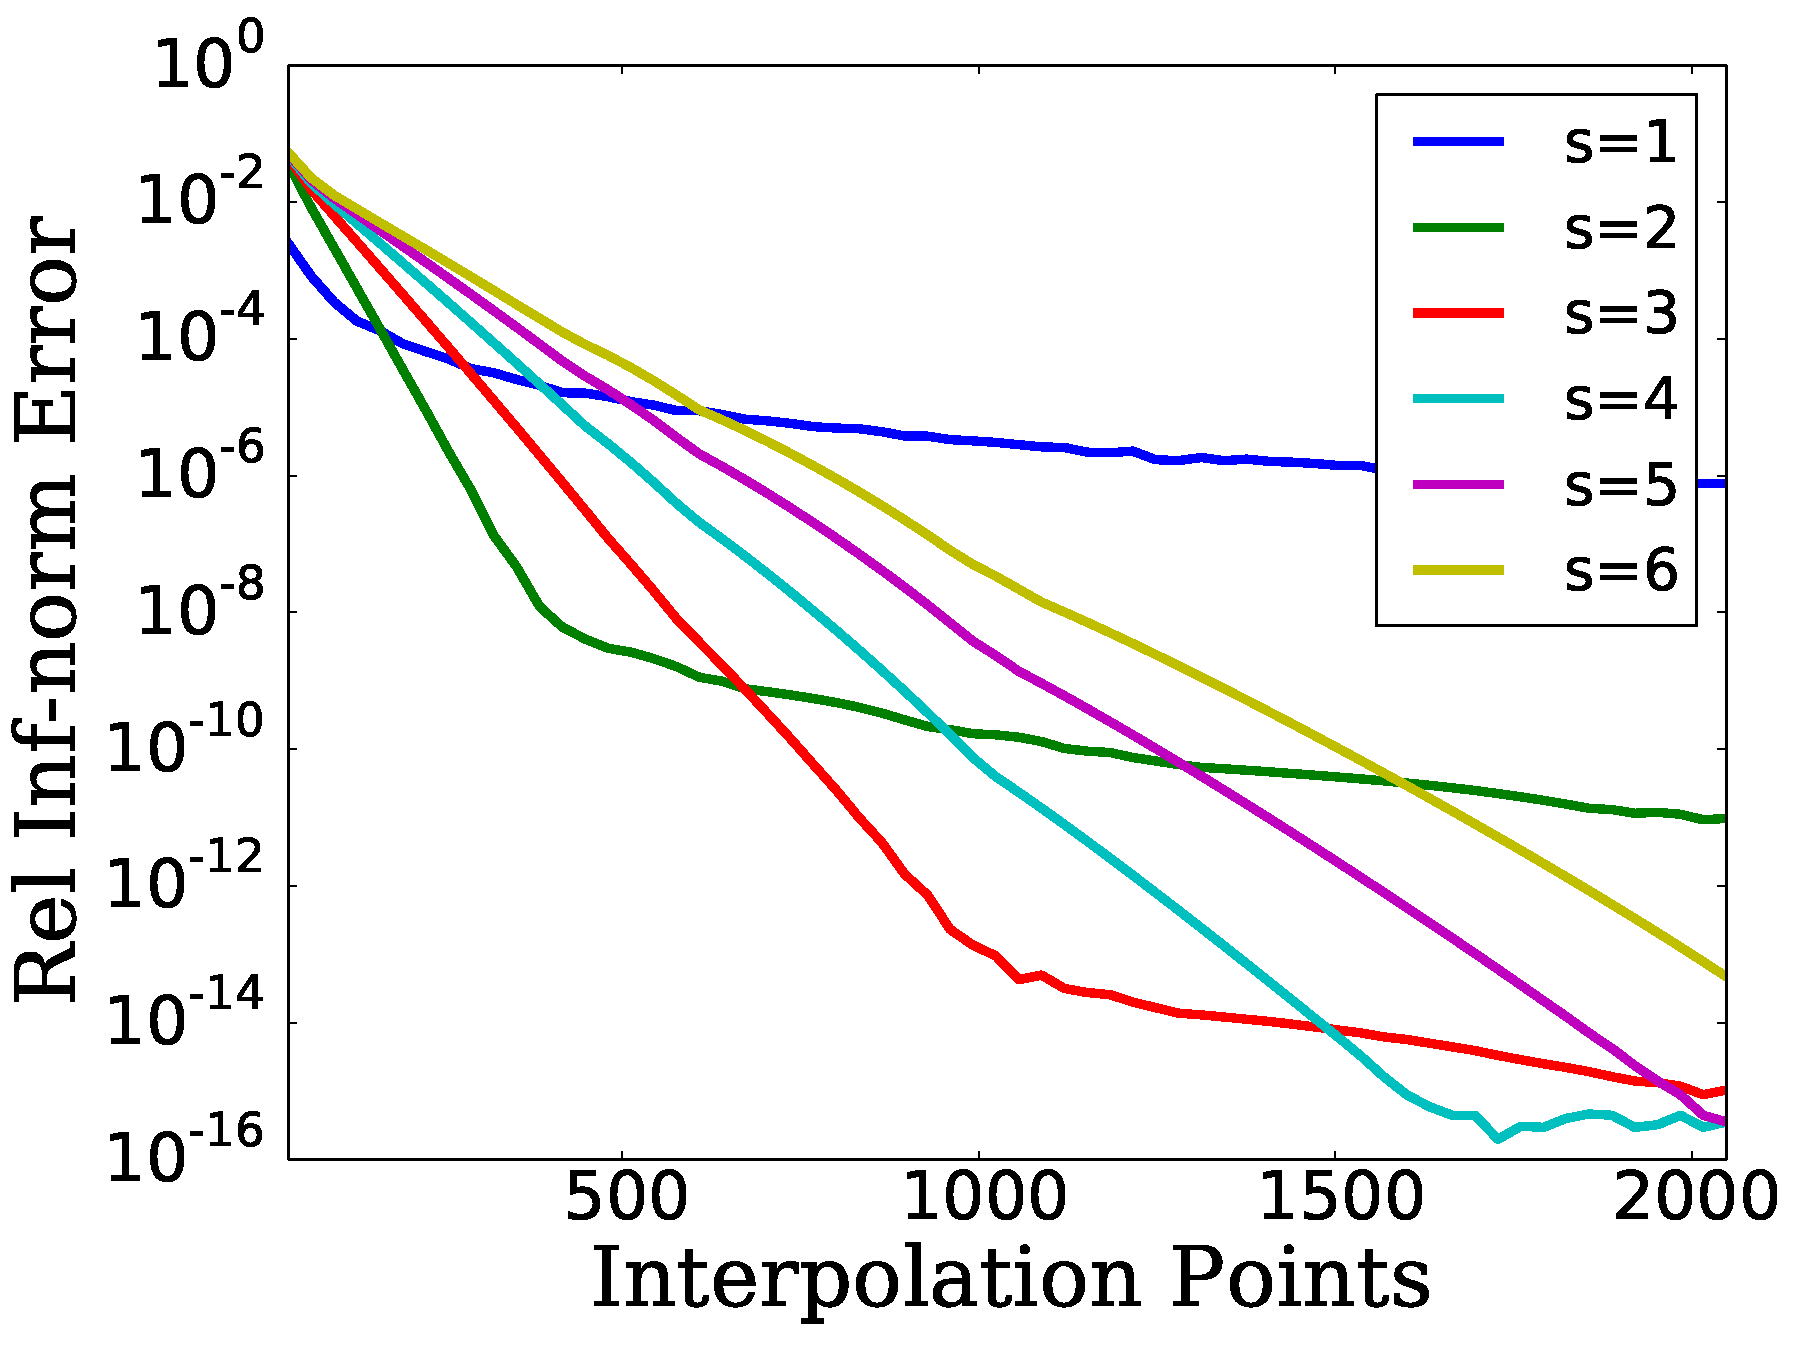
\includegraphics[width=\textwidth]{plots/msn_interp_fast_6n_rough_heaviside_2.pdf}
    \caption{Degree $6n$}
    \end{subfigure}
    \begin{subfigure}{0.45\textwidth}
    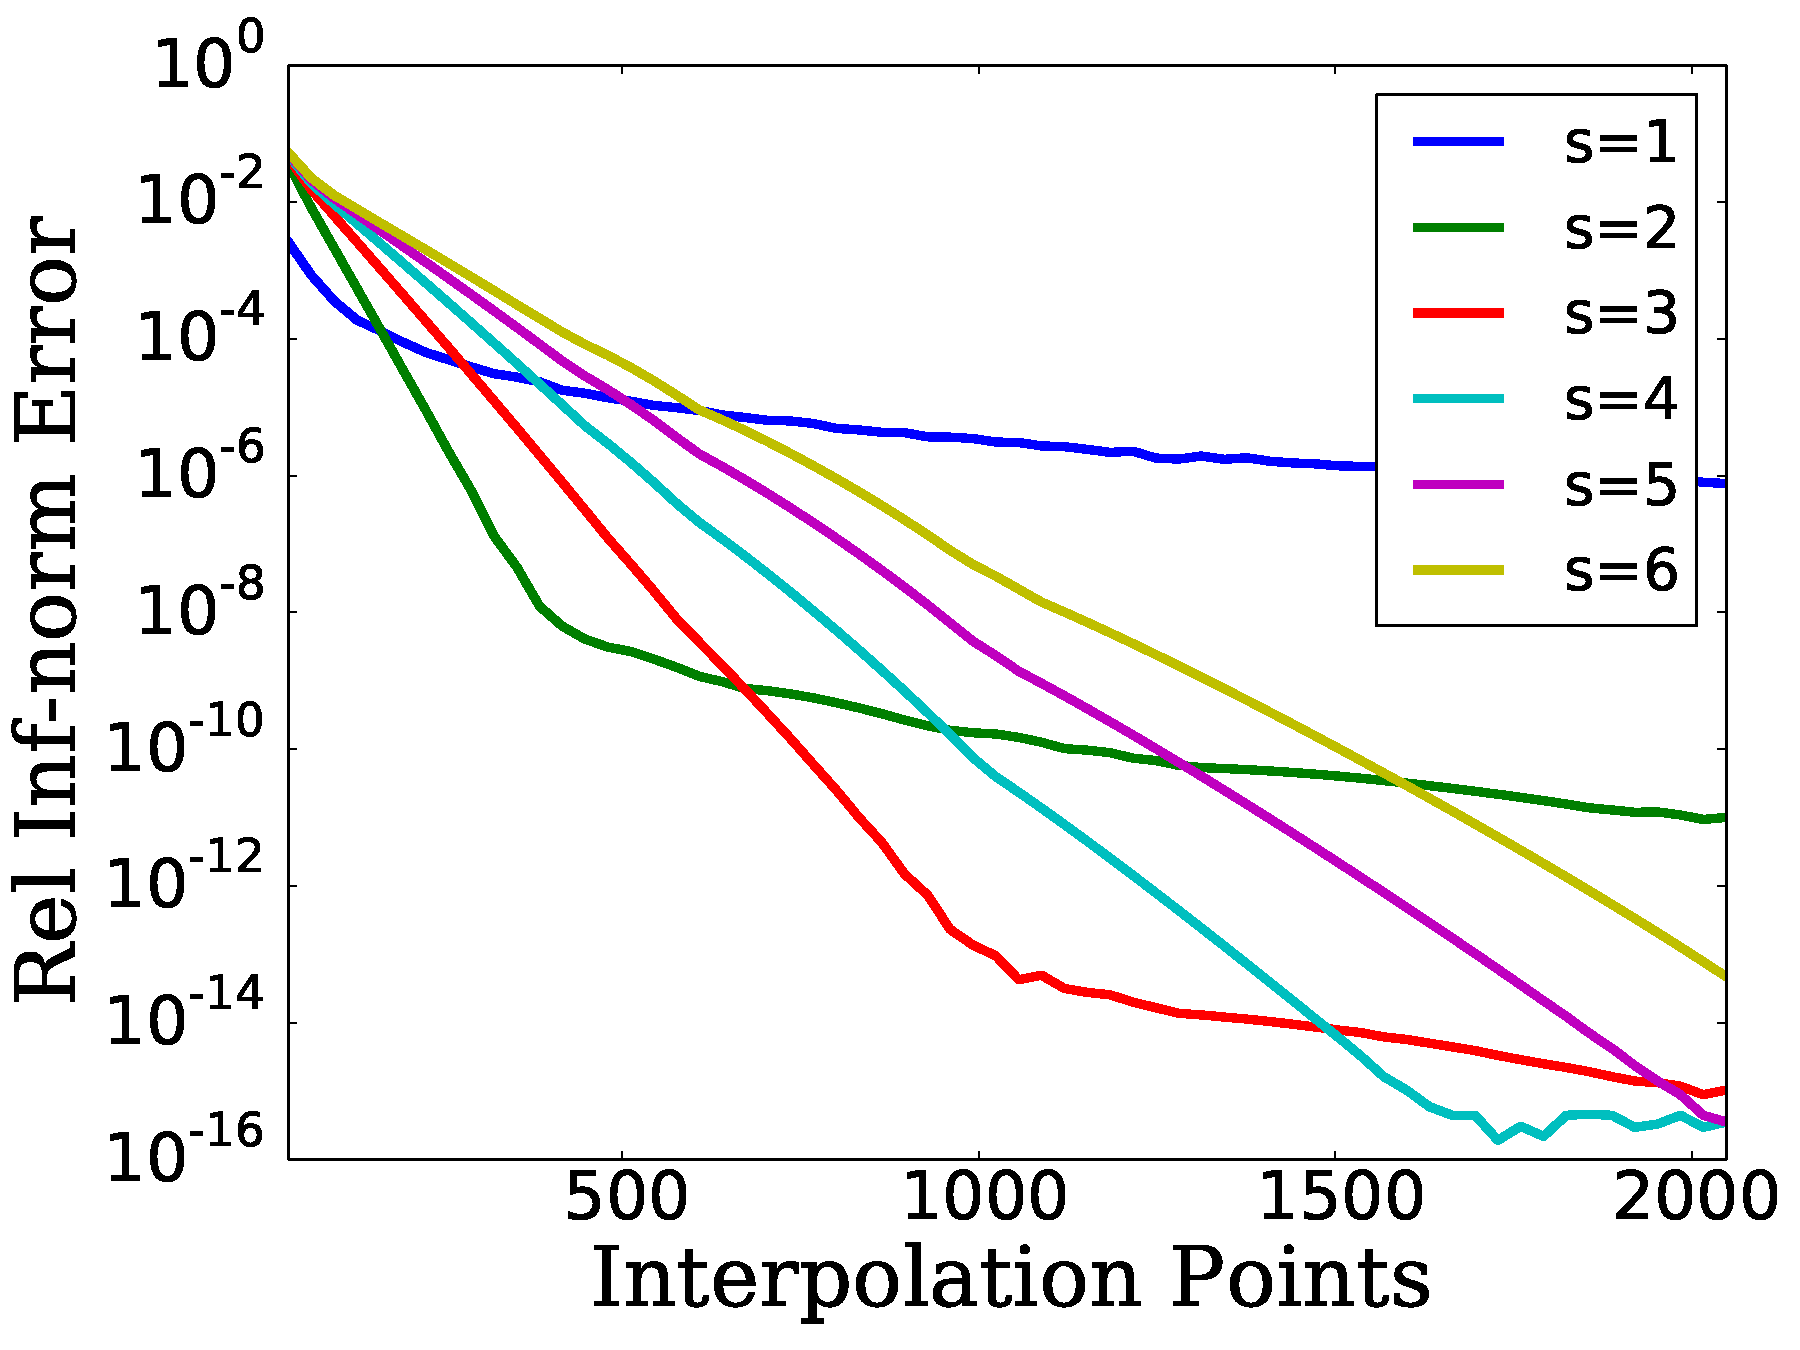
\includegraphics[width=\textwidth]{plots/msn_interp_fast_8n_rough_heaviside_2.pdf}
    \caption{Degree $8n$}
    \end{subfigure}
\caption[Example Plots of MSN Interpolation of Various Degrees]{
We show results for different interpolation degree.
For large $s$ values, there is no apparent advantage for using
a higher interpolation degree.
}
\label{fig:msn_comp_degree}
\end{figure}







\subsection{Birkhoff Interpolation Comparison}

We now look the Birkhoff interpolation problem when we have
a discontinuous derivative.
The results for interpolating $G(\cdot,0.5)$ can be found in 
Fig.~\ref{fig:rough_birkhoff_comparison_sharp_func};
we compare MSN interpolation results against applying standard
filters to the coefficients obtained from the solution
in Eq.~\eqref{eq:smooth_birkhoff_system}.
As we can see, MSN interpolation performs significantly better than
any of the filters; in fact, the MSN plot appears the same as
the corresponding plot in Fig.~\ref{fig:rough_comparison_sharp_func}
except for $s=1$.
Results for Birkhoff interpolation of $G_{2}(\cdot,0.5)$
can be found in Fig.~\ref{fig:rough_birkhoff_comparison_sharp_func_2}.
The results are nowhere near as good, and neither of the methods
(MSN or Chebyshev filters) perform well in this case.
Better results may be possible but likely require more
interpolation nodes.
In this case, even though the interpolation could be solved well
with MSN, in this case the Birkhoff interpolation problem 
for general functions cannot.

% Print results for comparing MSN with Heaviside jump function

\begin{figure}[p]
    \centering
    \begin{subfigure}{0.45\textwidth}
    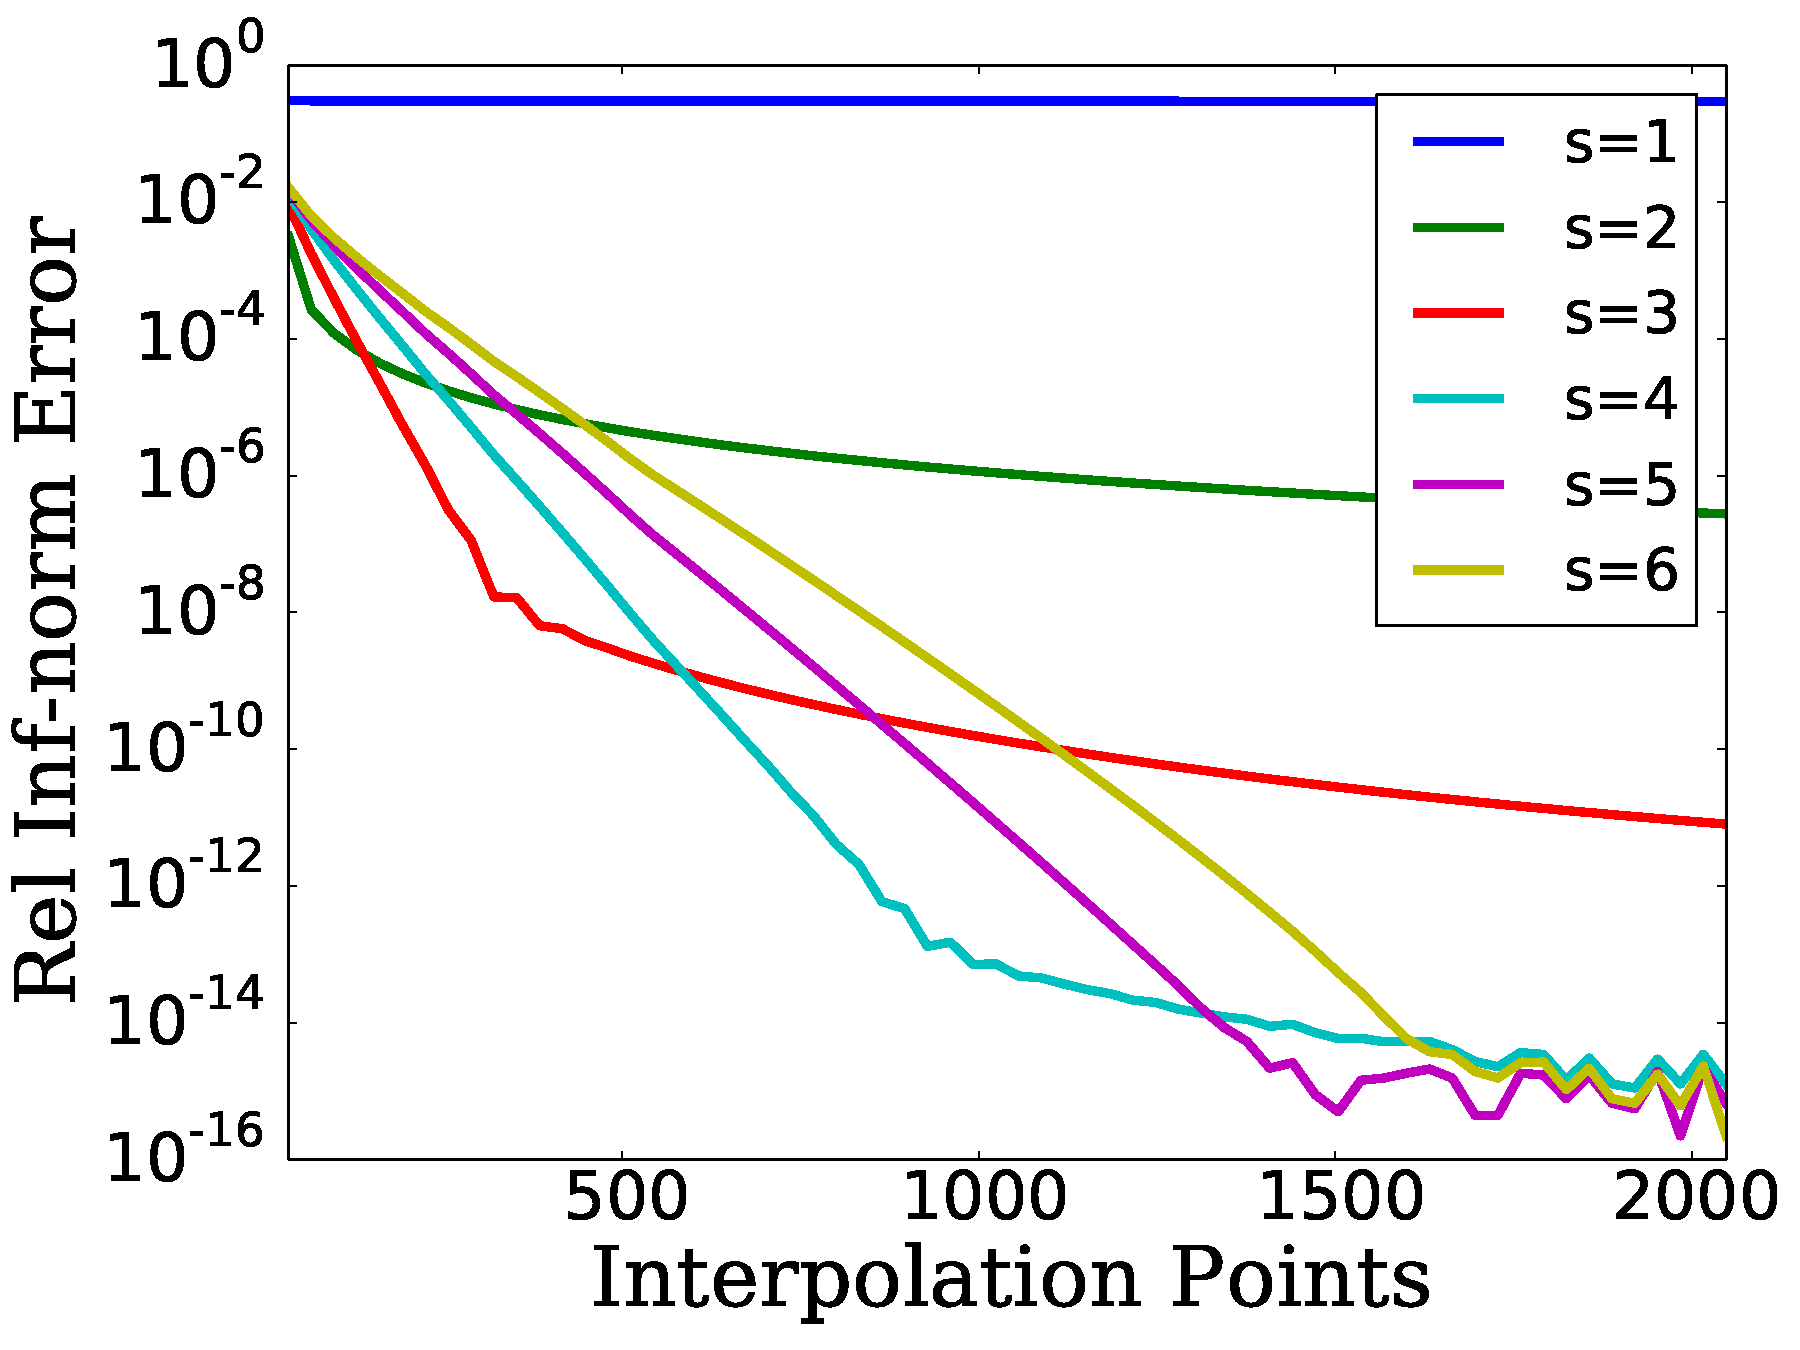
\includegraphics[width=\textwidth]{plots/msn_birkhoff_rough_sharp_funcs.pdf}
    \caption{MSN Interpolation}
    \end{subfigure}

    \begin{subfigure}{0.45\textwidth}
    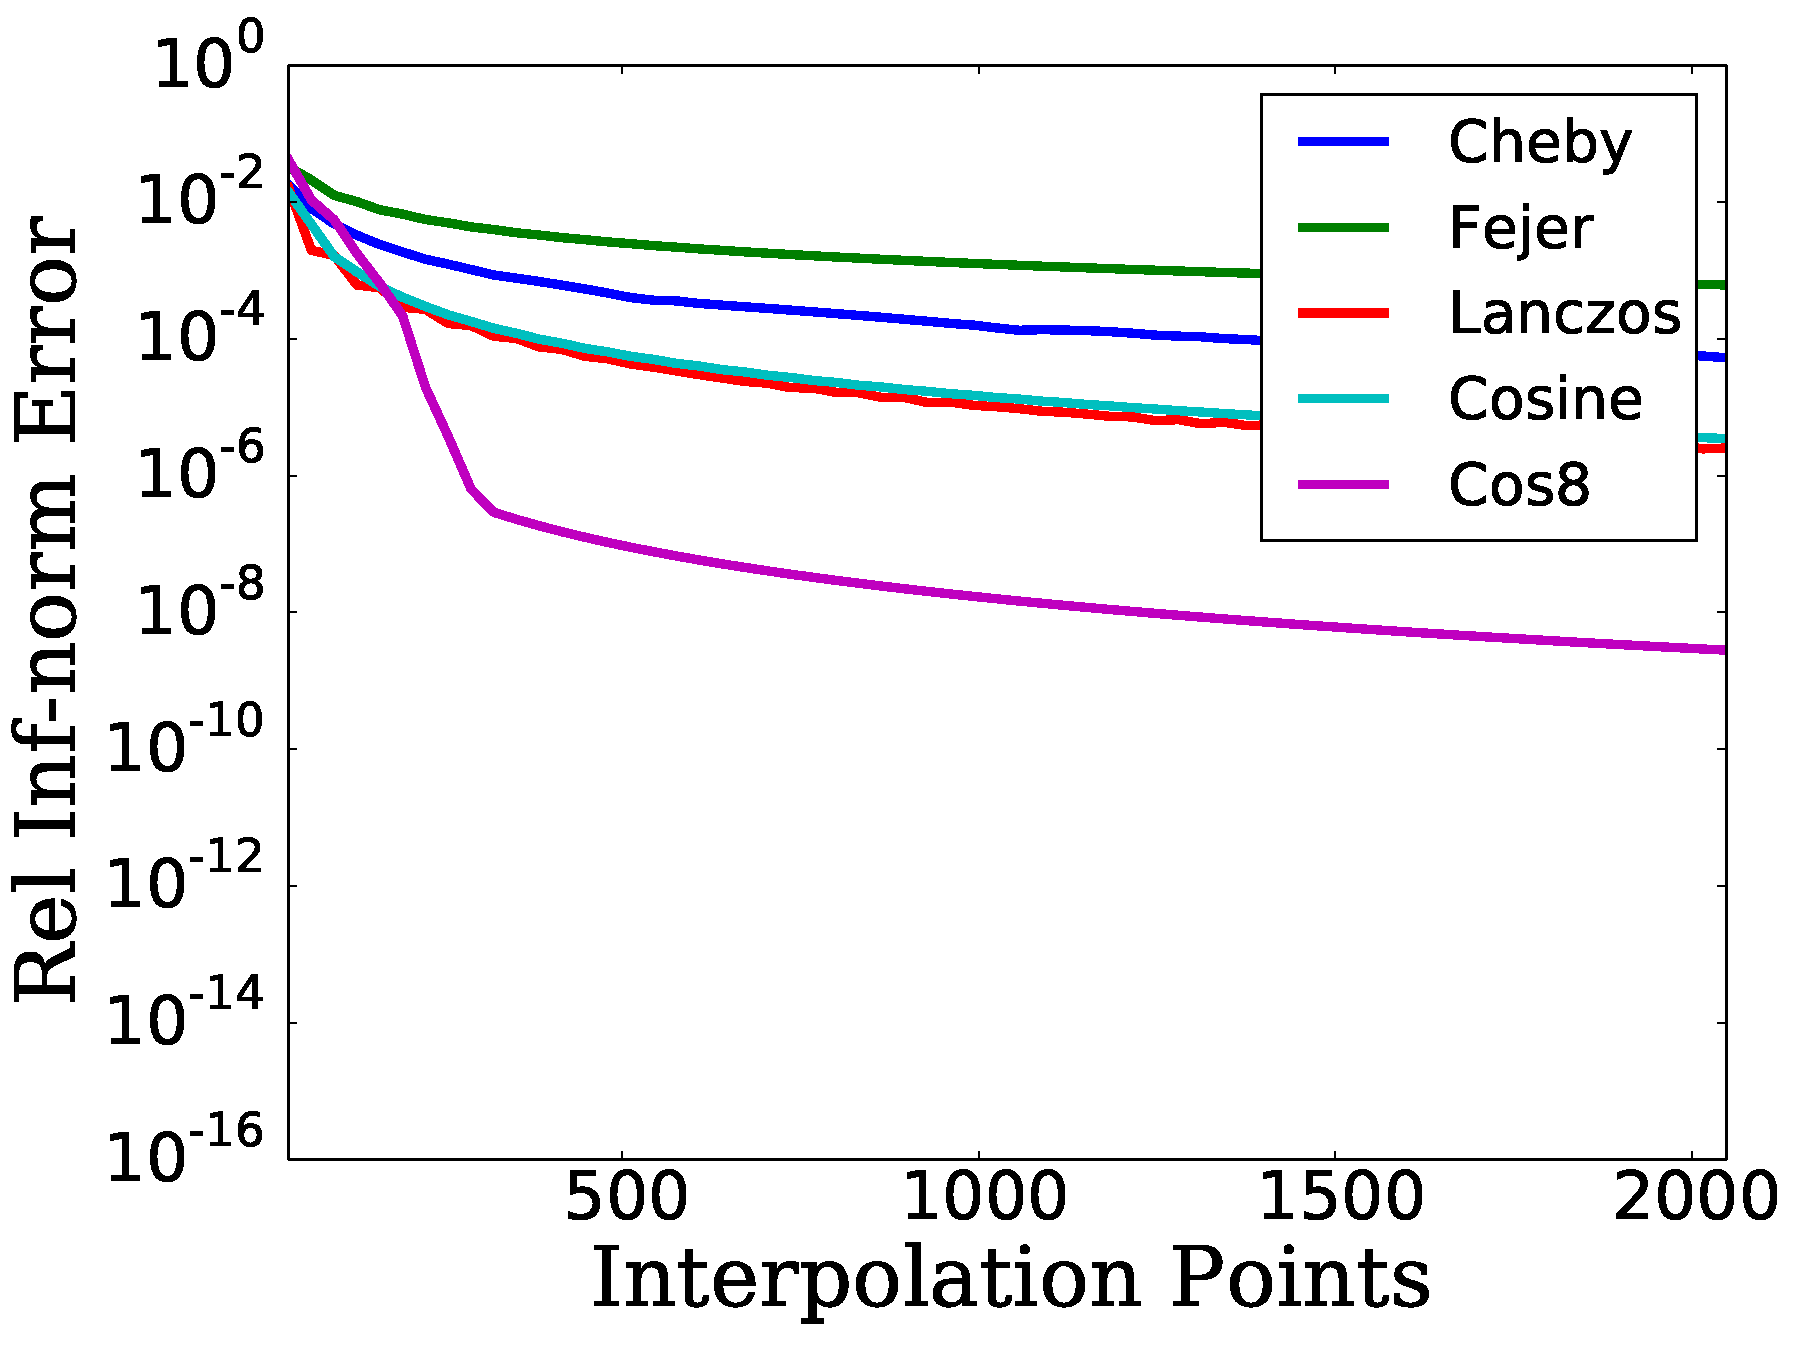
\includegraphics[width=\textwidth]{plots/cheby_birkhoff_filter_rough_sharp_func.pdf}
    \caption{Filters, Plot 1}
    \end{subfigure}
    \begin{subfigure}{0.45\textwidth}
    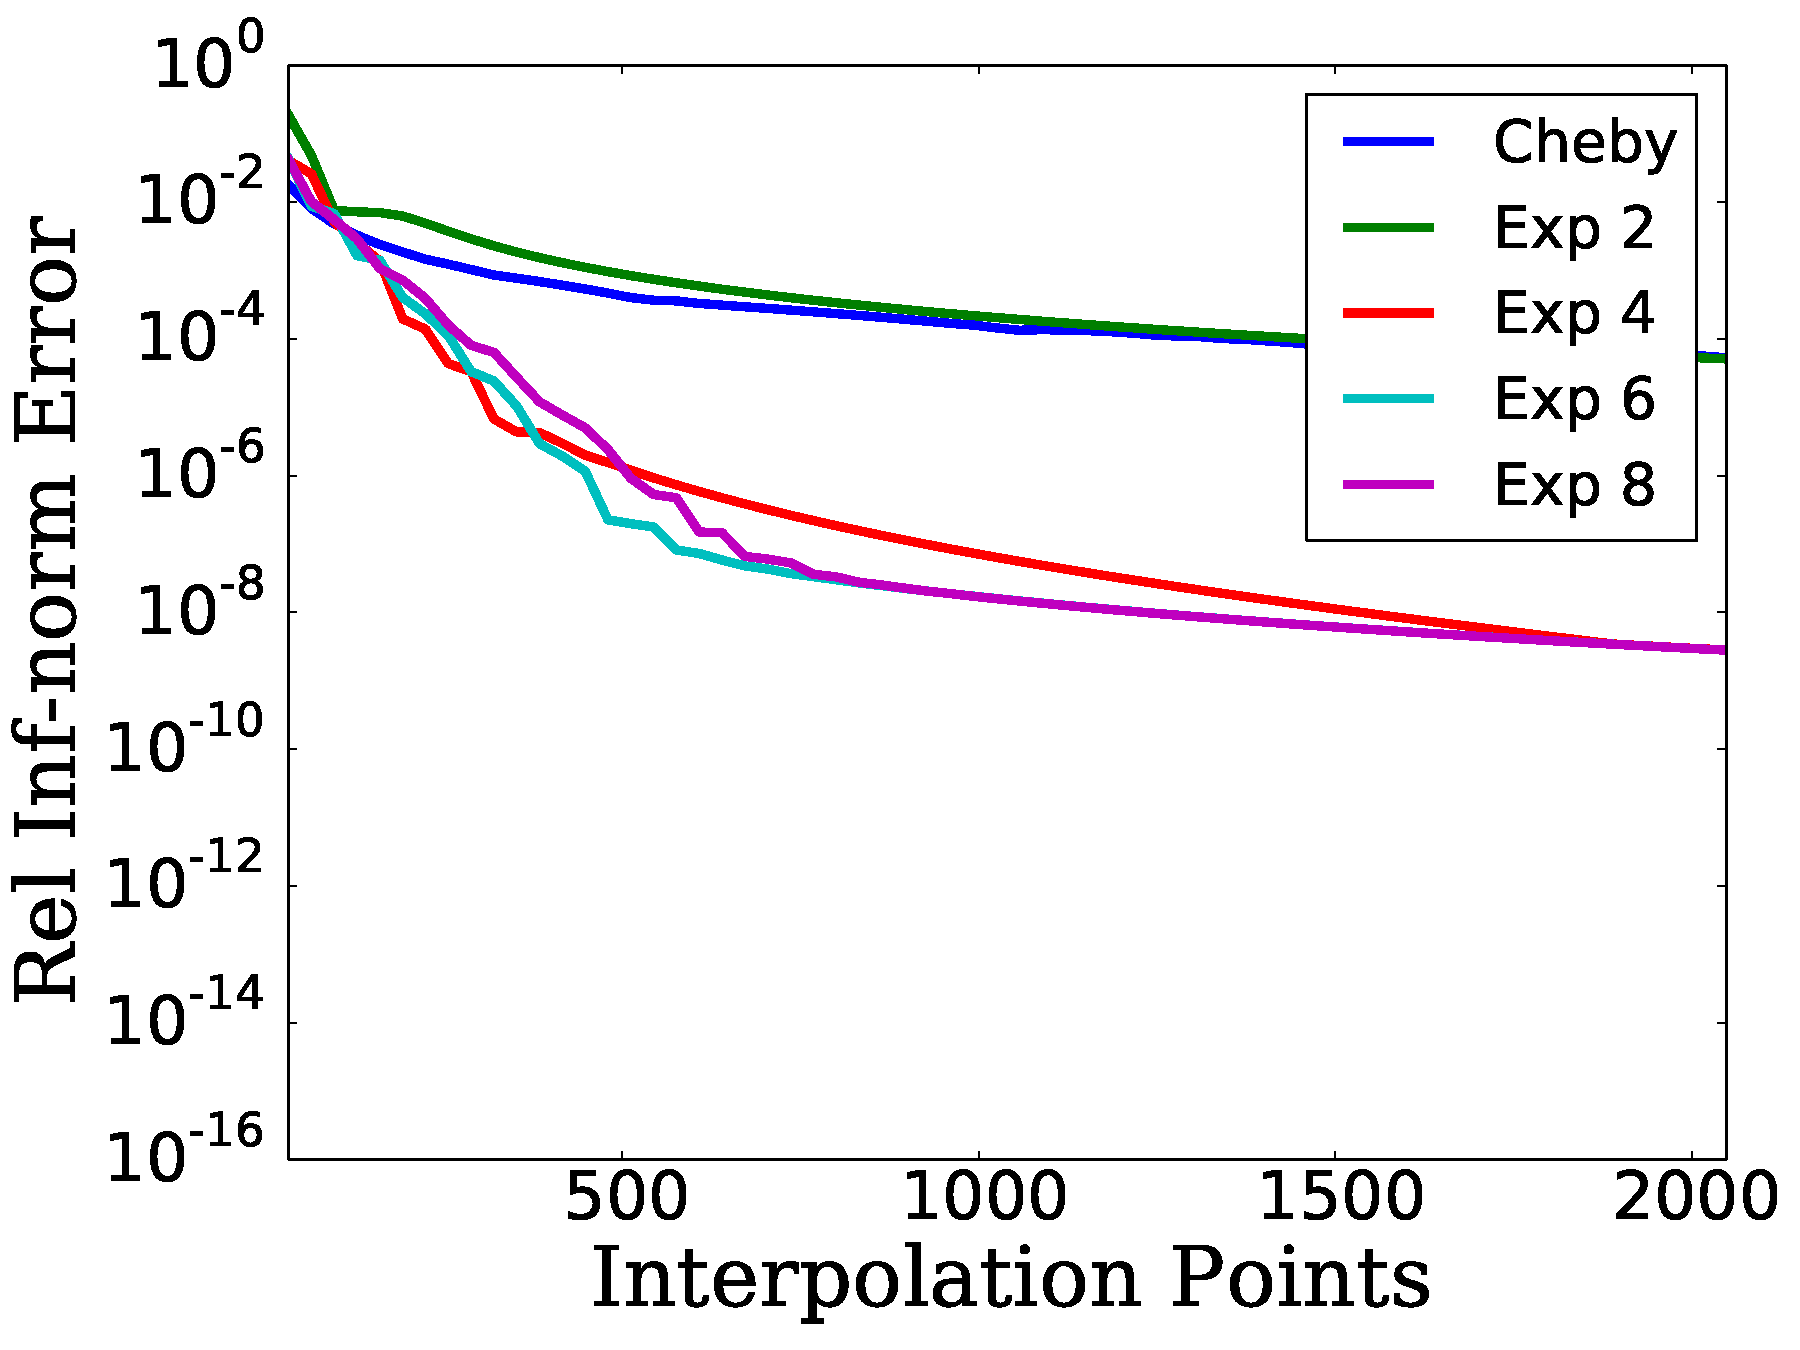
\includegraphics[width=\textwidth]{plots/cheby_birkhoff_filter_2_rough_sharp_func.pdf}
    \caption{Filters, Plot 2}
    \end{subfigure}
\caption[Rough Birkhoff Interpolation Comparison: Sharp Function]{
MSN interpolation and Chebyshev filtering results of the Sharp Function
$G(\cdot,0.5)$ for various $s$ values and filters.
We include standard Chebyshev birkhoff interpolant in both filter
examples for reference.
}
\label{fig:rough_birkhoff_comparison_sharp_func}
\end{figure}




% Print results for comparing MSN with Heaviside jump function

\begin{figure}[p]
    \centering
    \begin{subfigure}{0.45\textwidth}
    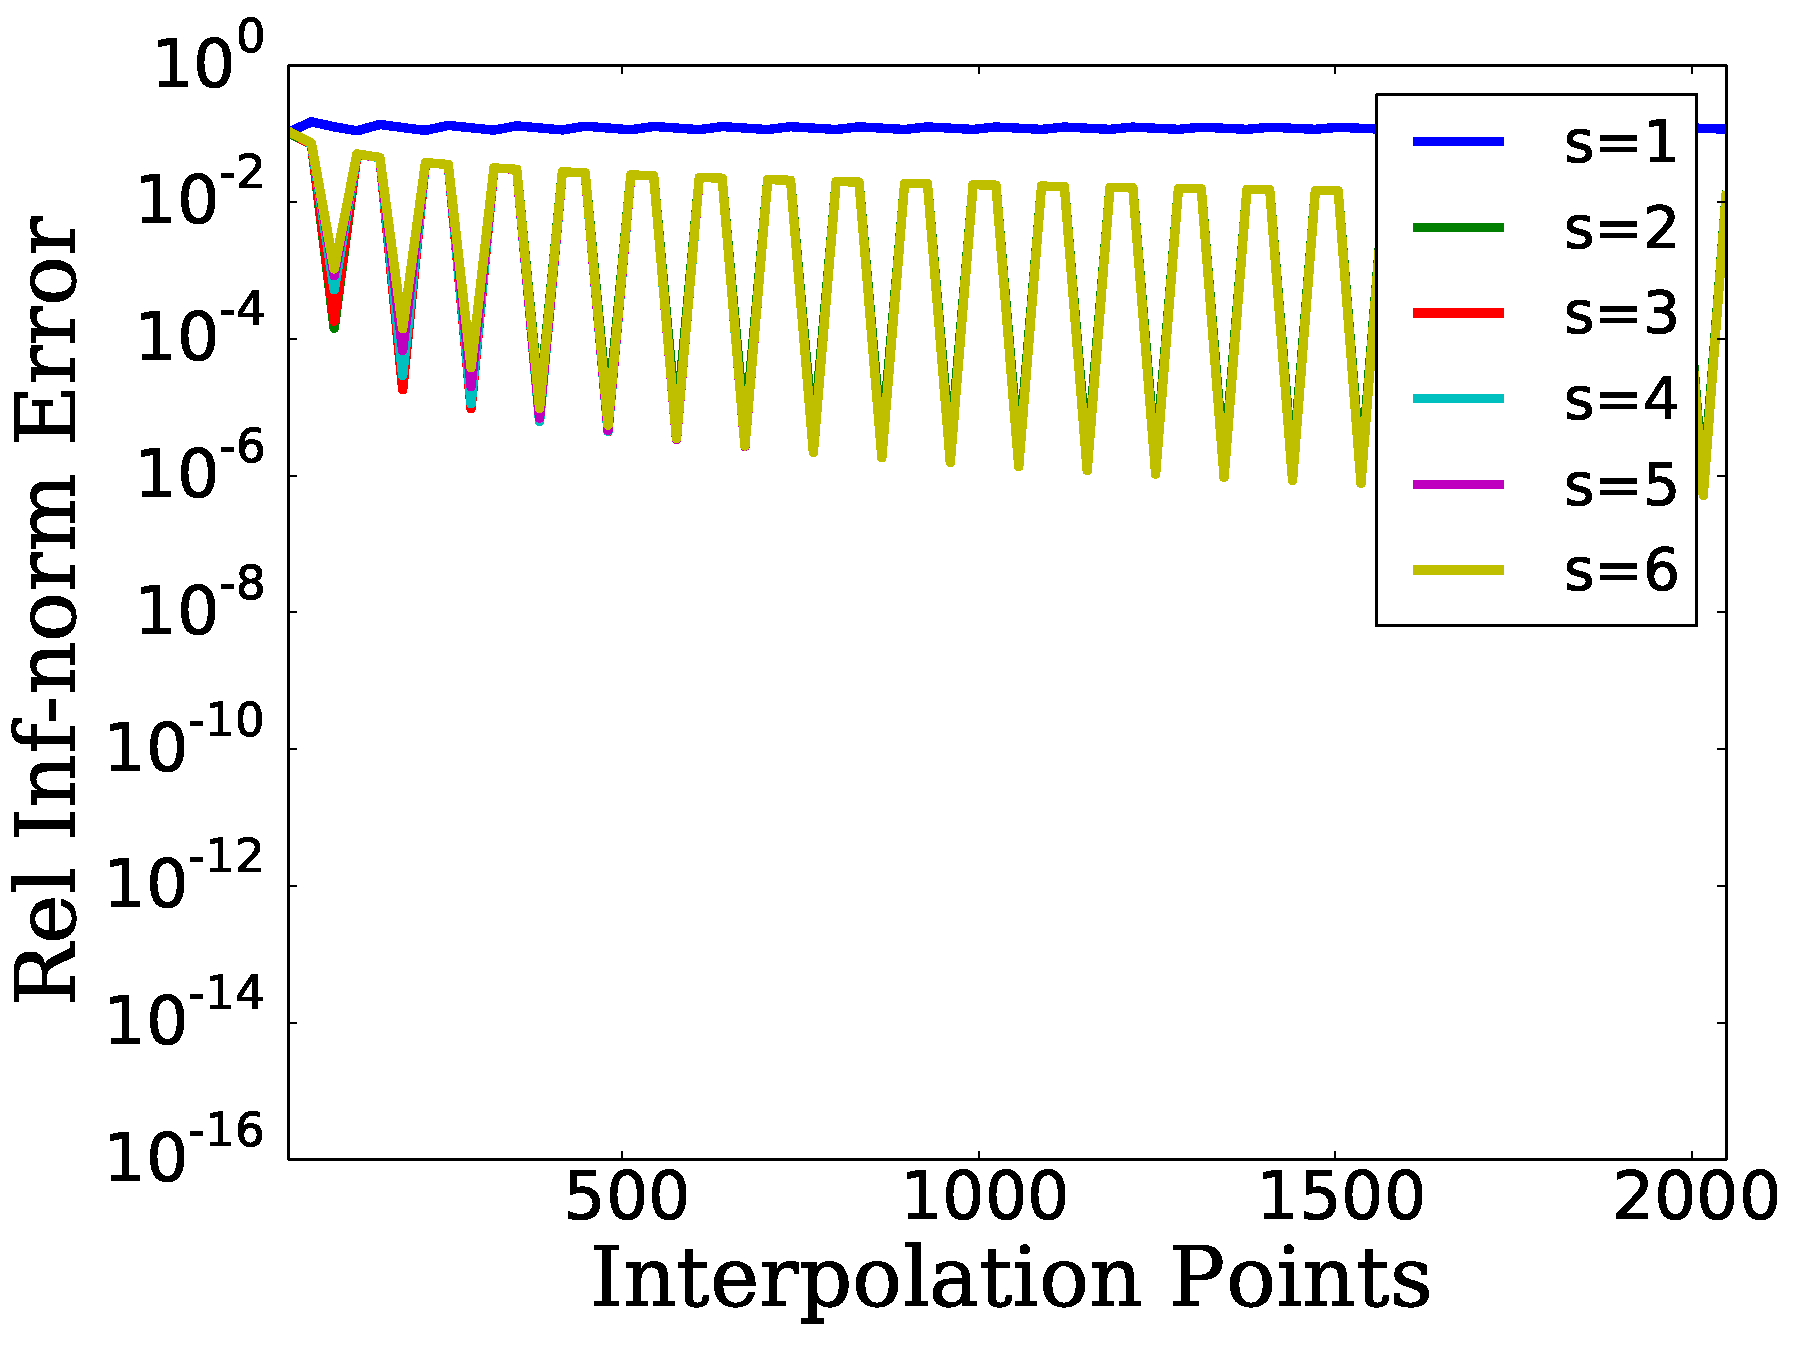
\includegraphics[width=\textwidth]{plots/msn_birkhoff_rough_sharp_funcs_2.pdf}
    \caption{MSN Interpolation}
    \end{subfigure}

    \begin{subfigure}{0.45\textwidth}
    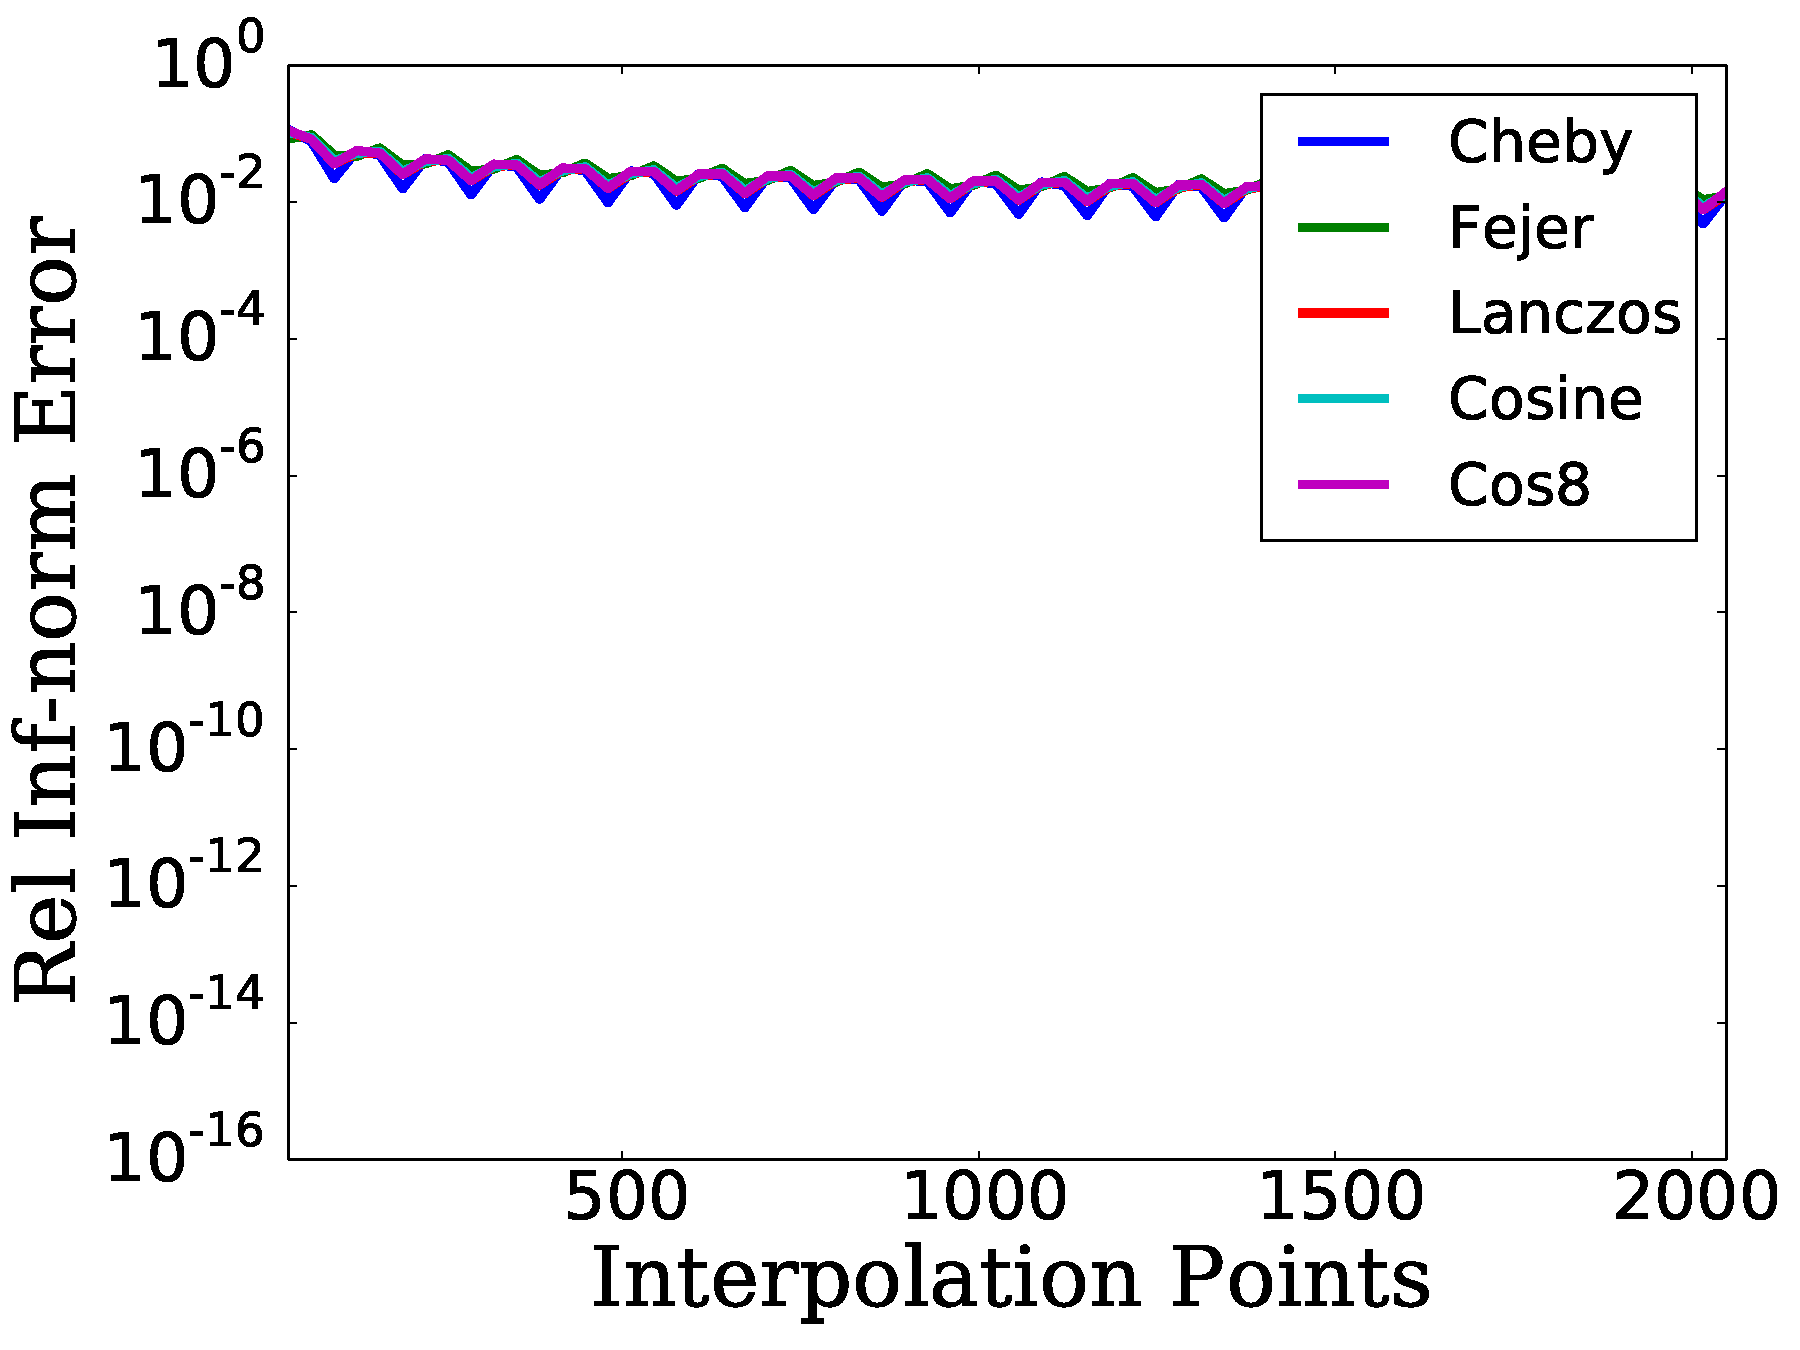
\includegraphics[width=\textwidth]{plots/cheby_birkhoff_filter_rough_sharp_func_2.pdf}
    \caption{Filters, Plot 1}
    \end{subfigure}
    \begin{subfigure}{0.45\textwidth}
    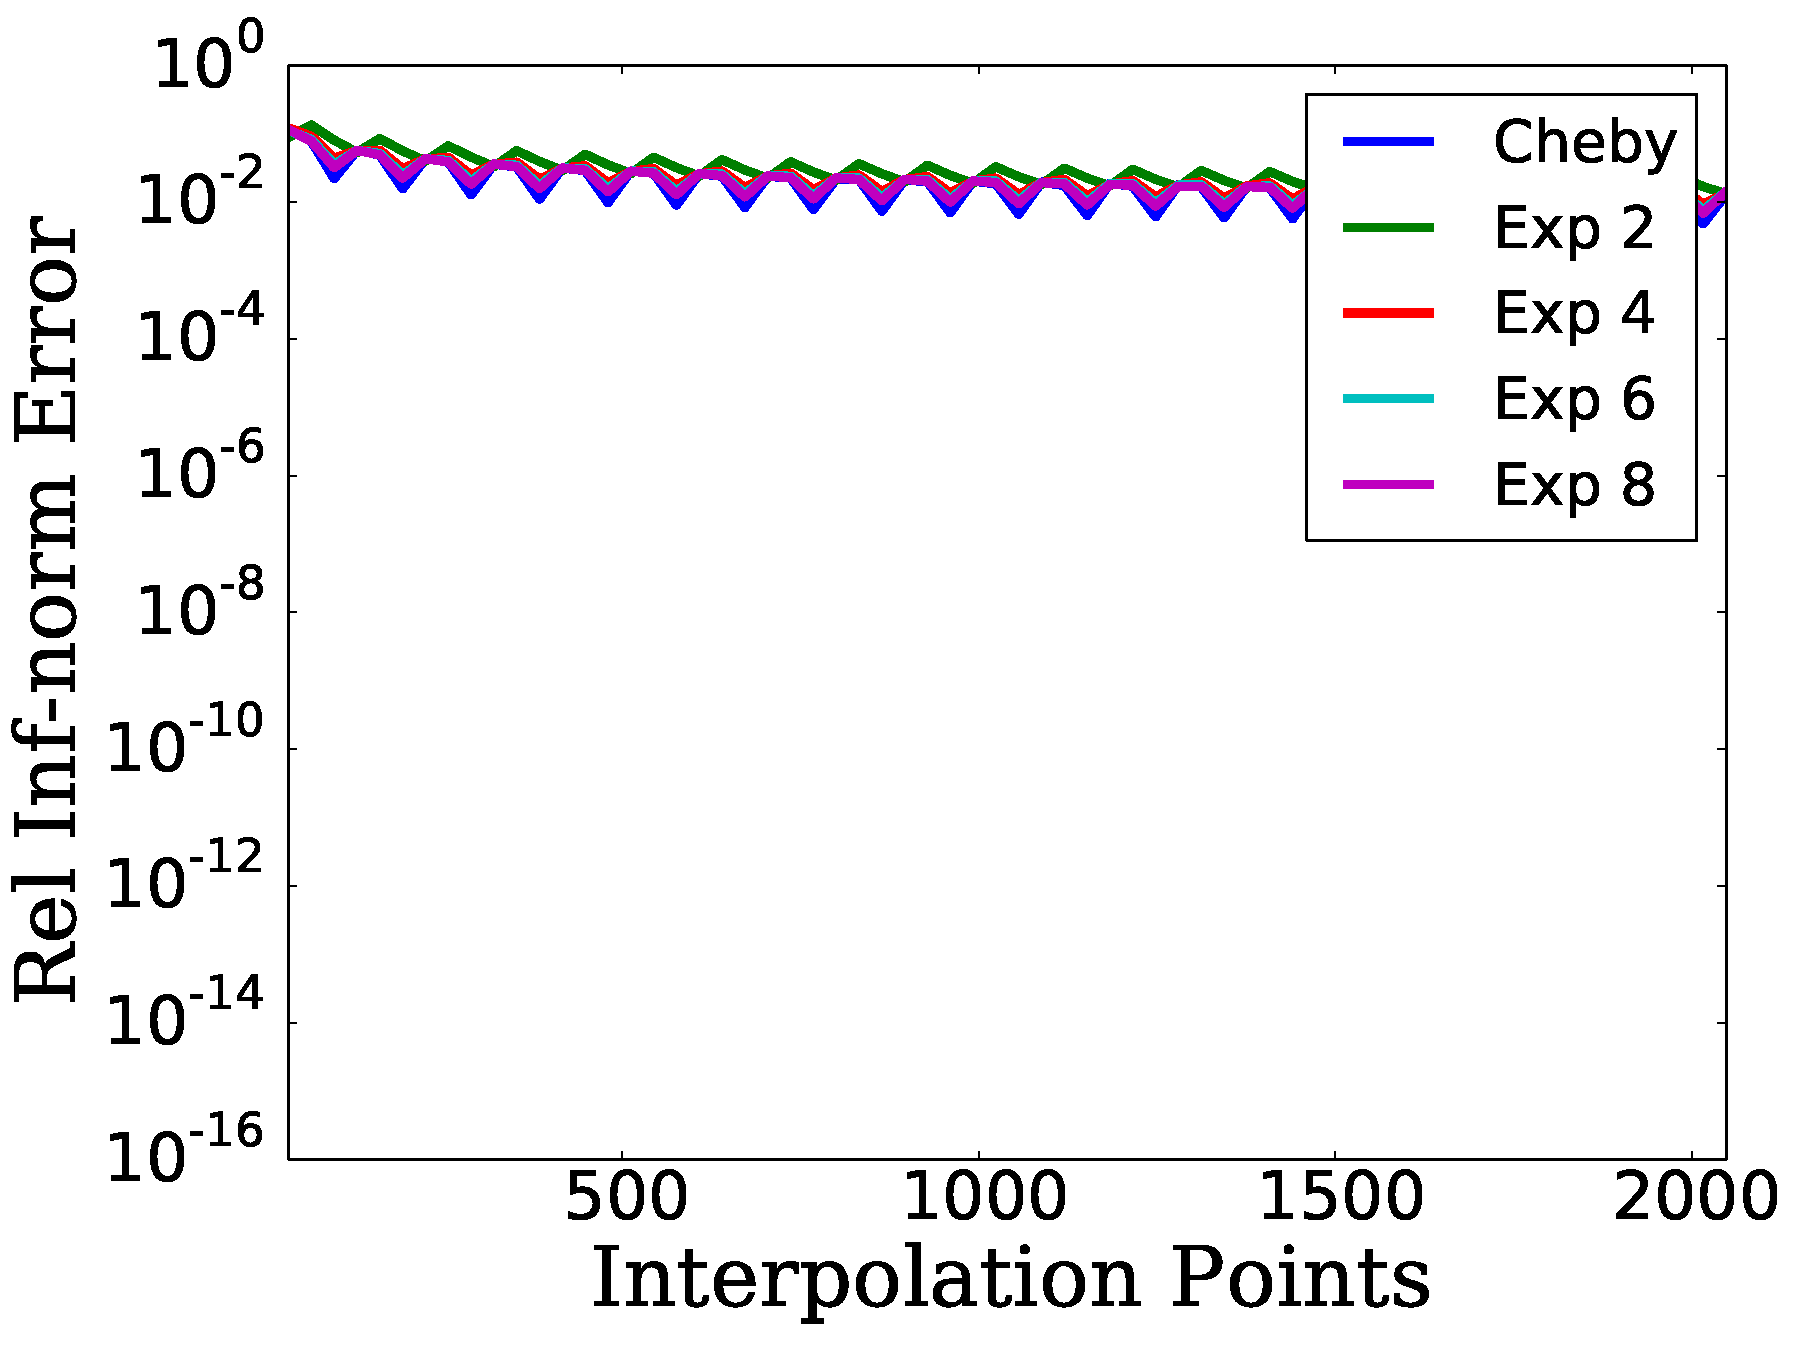
\includegraphics[width=\textwidth]{plots/cheby_birkhoff_filter_2_rough_sharp_func_2.pdf}
    \caption{Filters, Plot 2}
    \end{subfigure}
\caption[Rough Birkhoff Interpolation Comparison: Sharp Function 2]{
MSN interpolation and Chebyshev filtering results of the Sharp Function
$G_{2}(\cdot,0.5)$ for various $s$ values and filters.
We include standard Chebyshev birkhoff interpolant in both filter
examples for reference.
}
\label{fig:rough_birkhoff_comparison_sharp_func_2}
\end{figure}






%\section{Results for Fast MSN Interpolation in 2D for Rough Functions}
\label{sec:rough_2D_sim}

We now look at interpolation results of rough functions in 2D.
We will attempt to interpolate the following functions:
%
\begin{align}
    J(x,y) &= H(y-\sin(\pi x)) + H(y-x^{2}) \nonumber\\
    S(x,y,\alpha) &= G(y-\sin(\pi x),\alpha) + G(y-x^{2},\alpha).
\end{align}
%
Both $J$ and $S$ are challenging functions to interpolate,
as both have difficulties along the curves $y=\sin\pi x$ and $y=x^{2}$:
$J$ is discontinuous along those curves while $S(\cdot,\cdot,\alpha)$
has infinite derivatives.

% ^^^ Ignored for right now.


